\chapter{Desarrollo Experimental}
Para el siguiente proyecto se utilizaron como base celdas electroquímicas impresas en carbono por el método de serigrafía sobre un sustrato Valox (Figura ~\ref{fig:Figura_Electrodos_nPOC}). Mediante una impresora marca Fujifilm modelo Dimatix DMP-2850 se realizó la deposición de la tinta de oro sobre el electrodo de trabajo. Se caracterizaron las propiedades eléctricas, dimensionales y electroquímicas de la misma para corroborar el correcto funcionamiento de los sensores.

\begin{figure}[H]
  \centering
    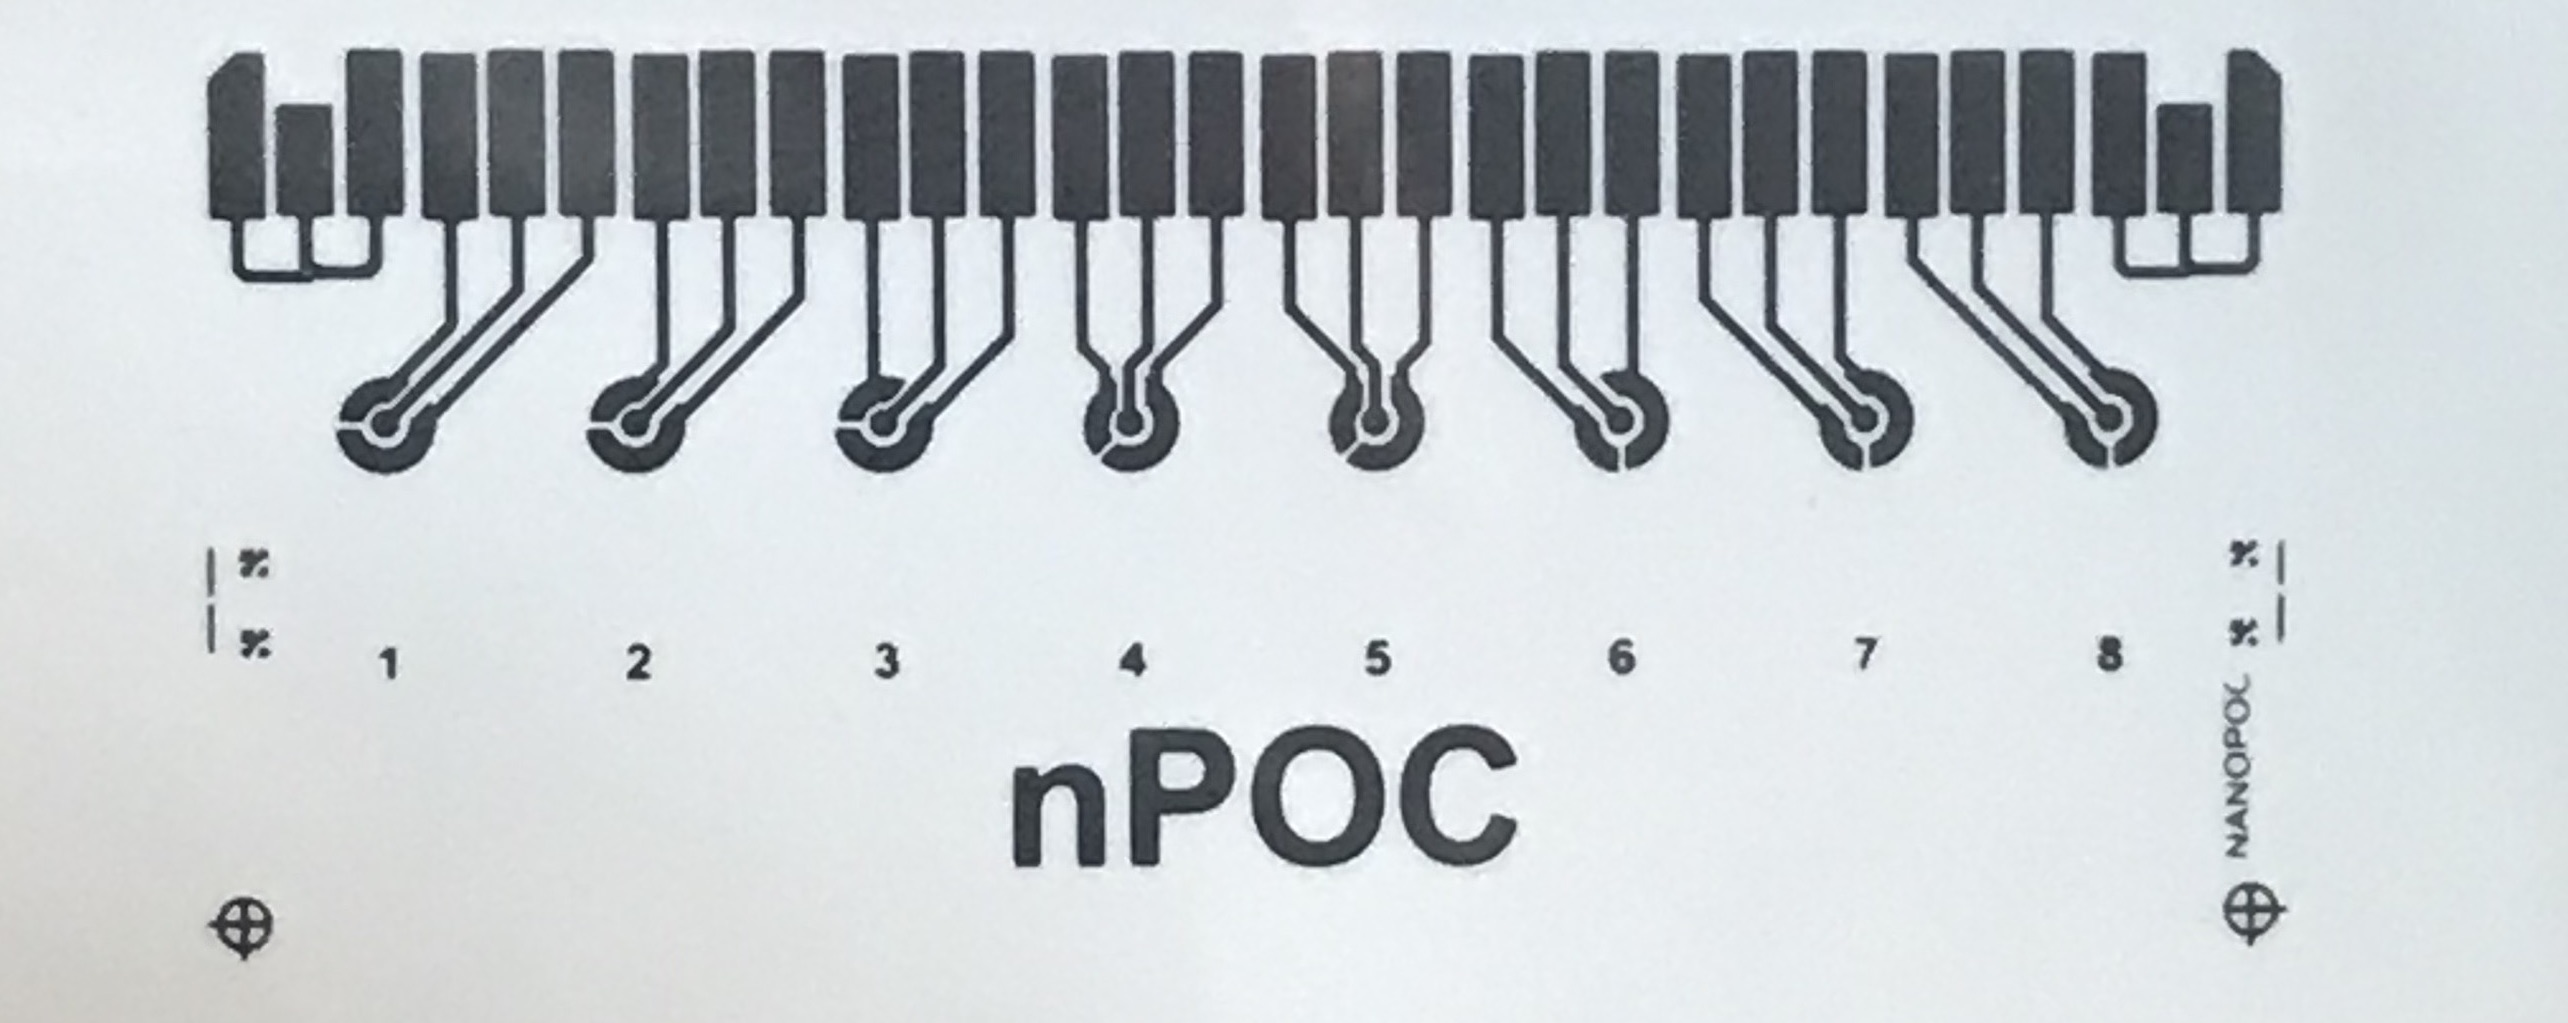
\includegraphics[width=0.5\textwidth]{Figuras/Figura_Electrodos_nPOC}
  \caption{Celdas Electroqu\'imicas}
  \label{fig:Figura_Electrodos_nPOC}
\end{figure}

\section{Preparación de patrones de imágenes}

\subsection{Mediciones previas}
Como primera instancia, se midieron los diferentes componentes de las celdas electroquímicas impresos en carbono. Se concluyó que los electrodos de trabajo (desde ahora \emph{WE}) poseen 1 mm de diámetro, donde se depositará la tinta de oro. La separación entre \emph{WE} y electrodo de referencia (desde ahora \emph{RE}) y contraelectrodo (desde ahora \emph{CE}) es de 400 $\mu$m. La distancia entre dos \emph{WE} es de 9 mm y cada cartucho cuenta con ocho sensores. Esta distancia medida entre dos \emph{WE} corresponde a la separación de una micro pipeta de ocho canales, utilizada en laboratorios. (Figura ~\ref{fig:Figura_medicion_celdas})

\begin{figure}[H]
  \centering
    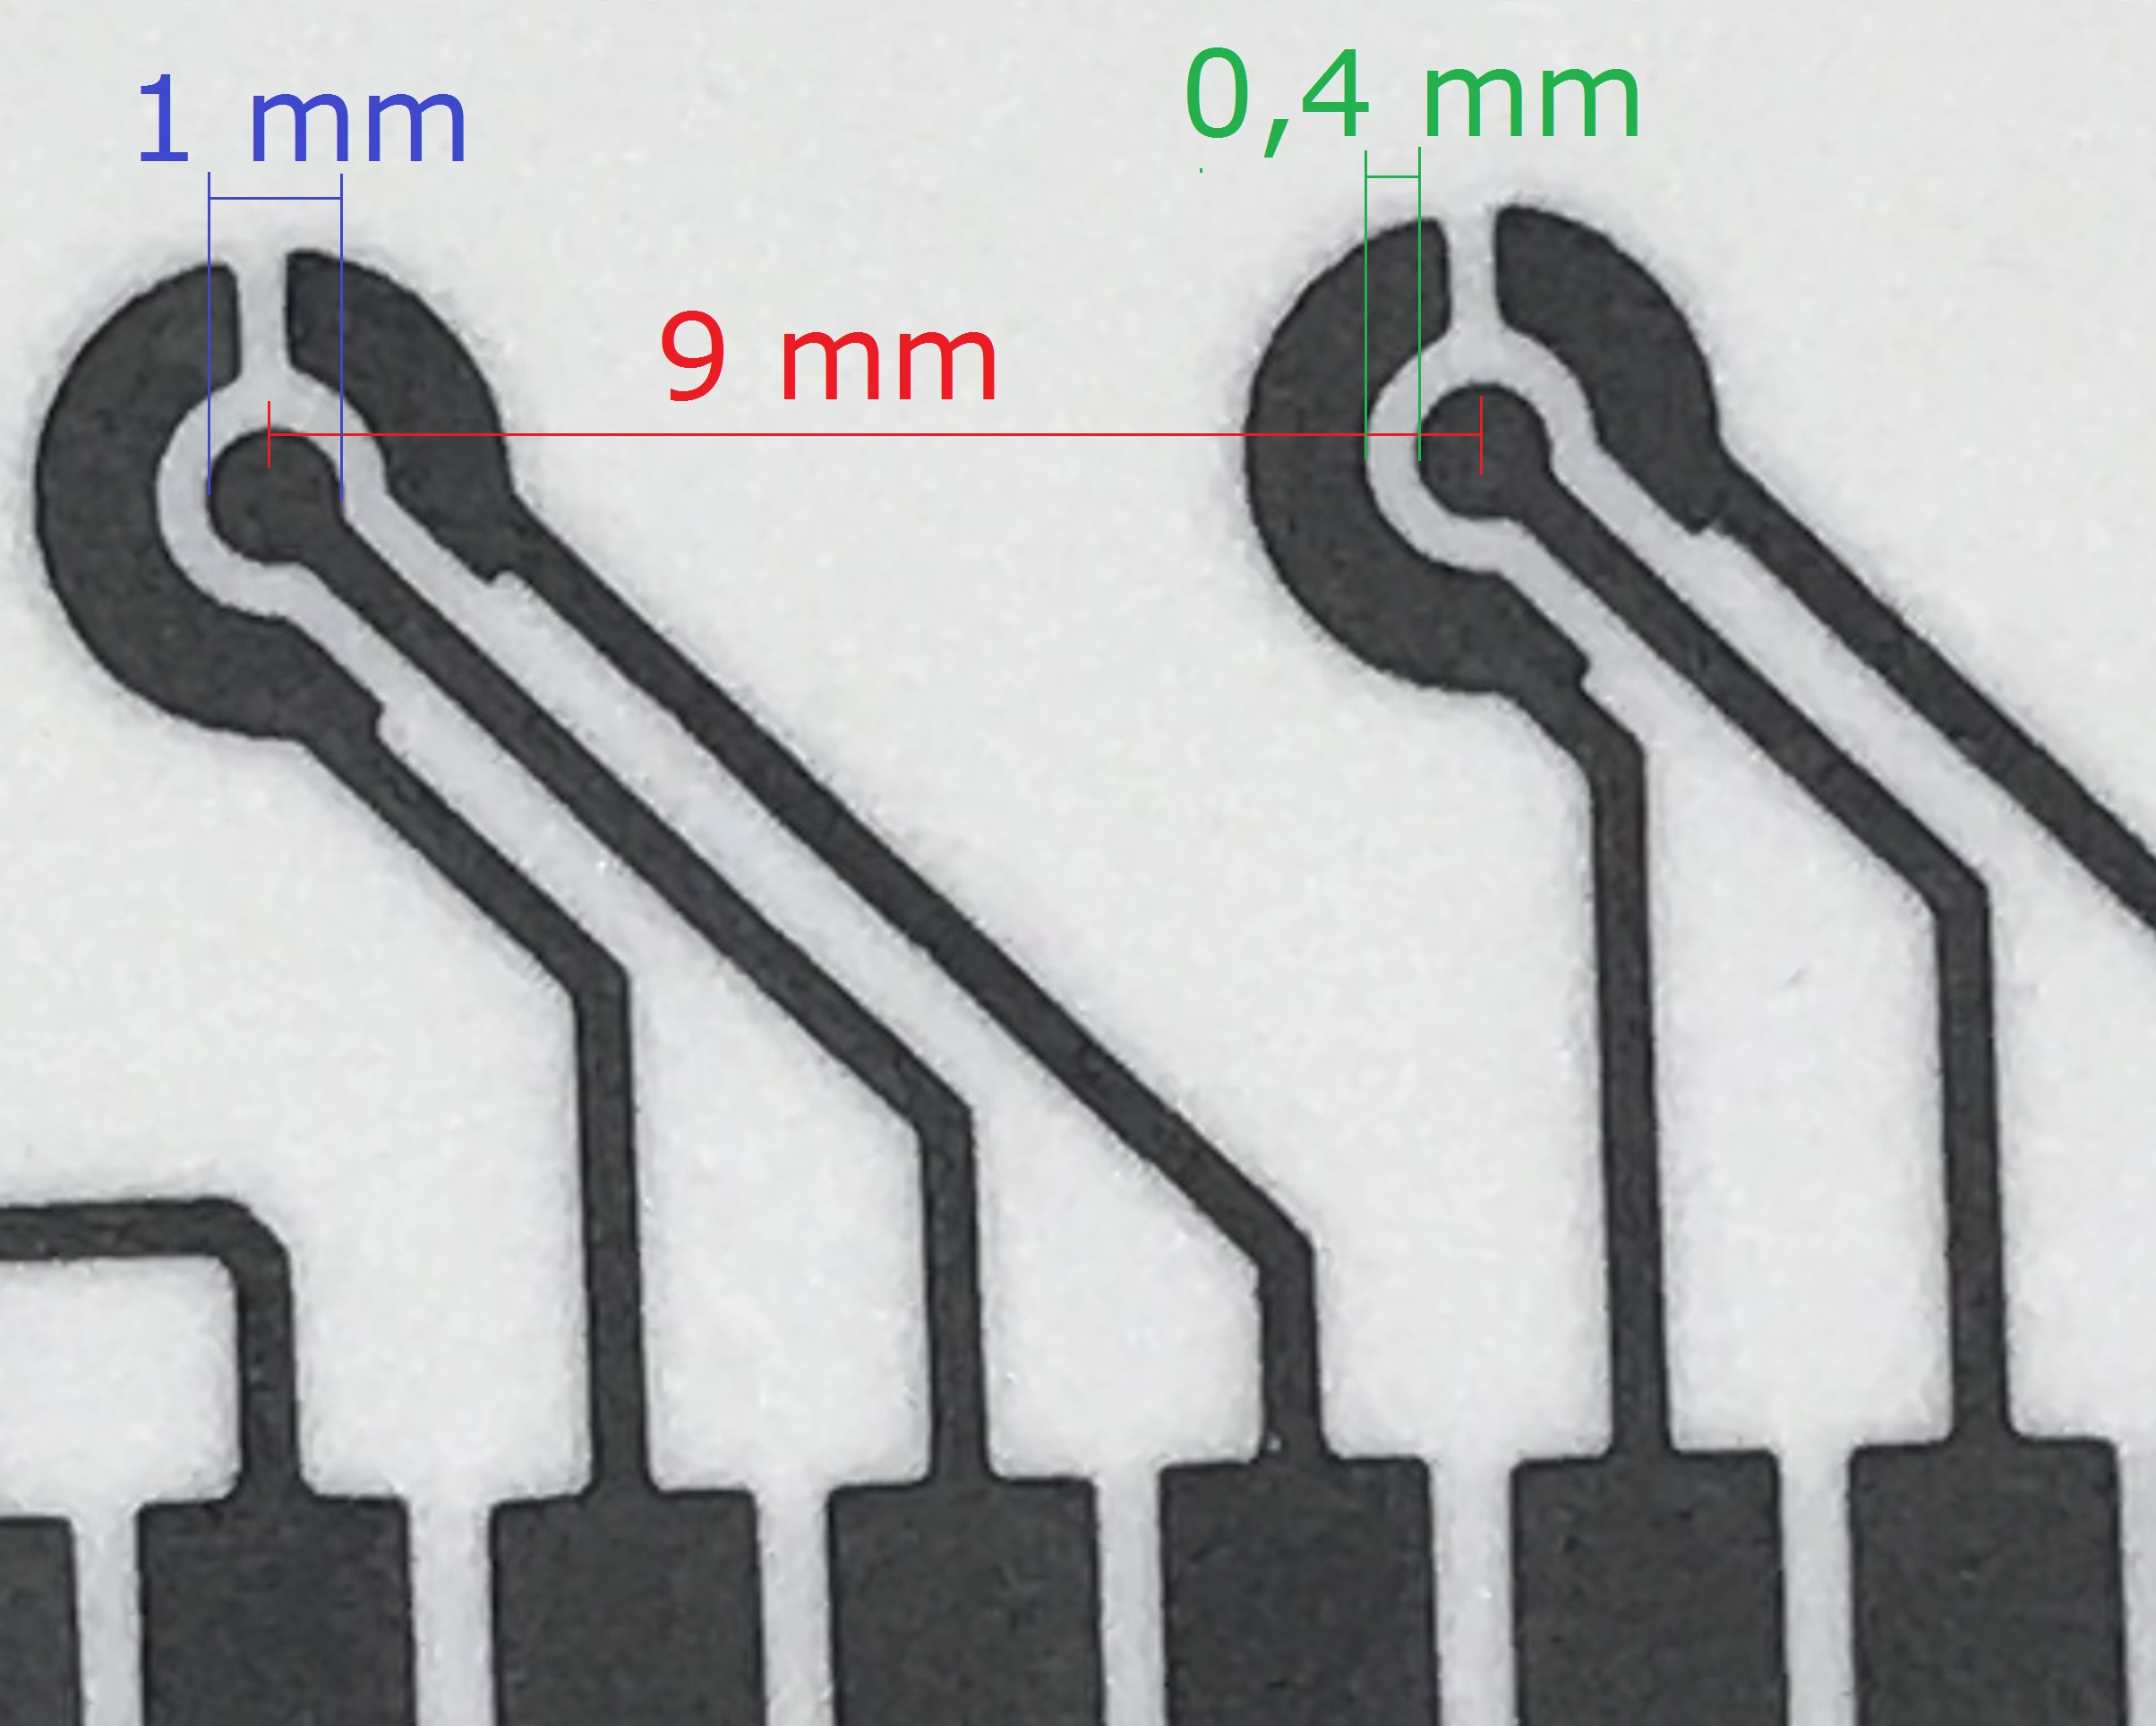
\includegraphics[width=0.5\textwidth]{Figuras/Figura_medicion_celdas}
  \caption{Mediciones dimensionales en sustrato.}
  \label{fig:Figura_medicion_celdas}
\end{figure}

Dado que las impresiones de carbono fueron realizadas por una empresa dedicada a impresiones serigráficas industriales, los biosensores se encuentran fabricados en dos columnas y seis filas dando un total de doce sensores por sustrato de tamaño A4 (Figura ~\ref{fig:Figura_sensores_hoja_A4}). Para tener un seguimiento preciso de los trabajos que se realizarán en cada muestra se los enumera aprovechando su nombre ya impreso en carbono como \textit{nPoc} del 1 al 5. (Figura ~\ref{fig:Figura_ejemplo_numeracion_nPoc})

\begin{figure}[H]
  \centering
    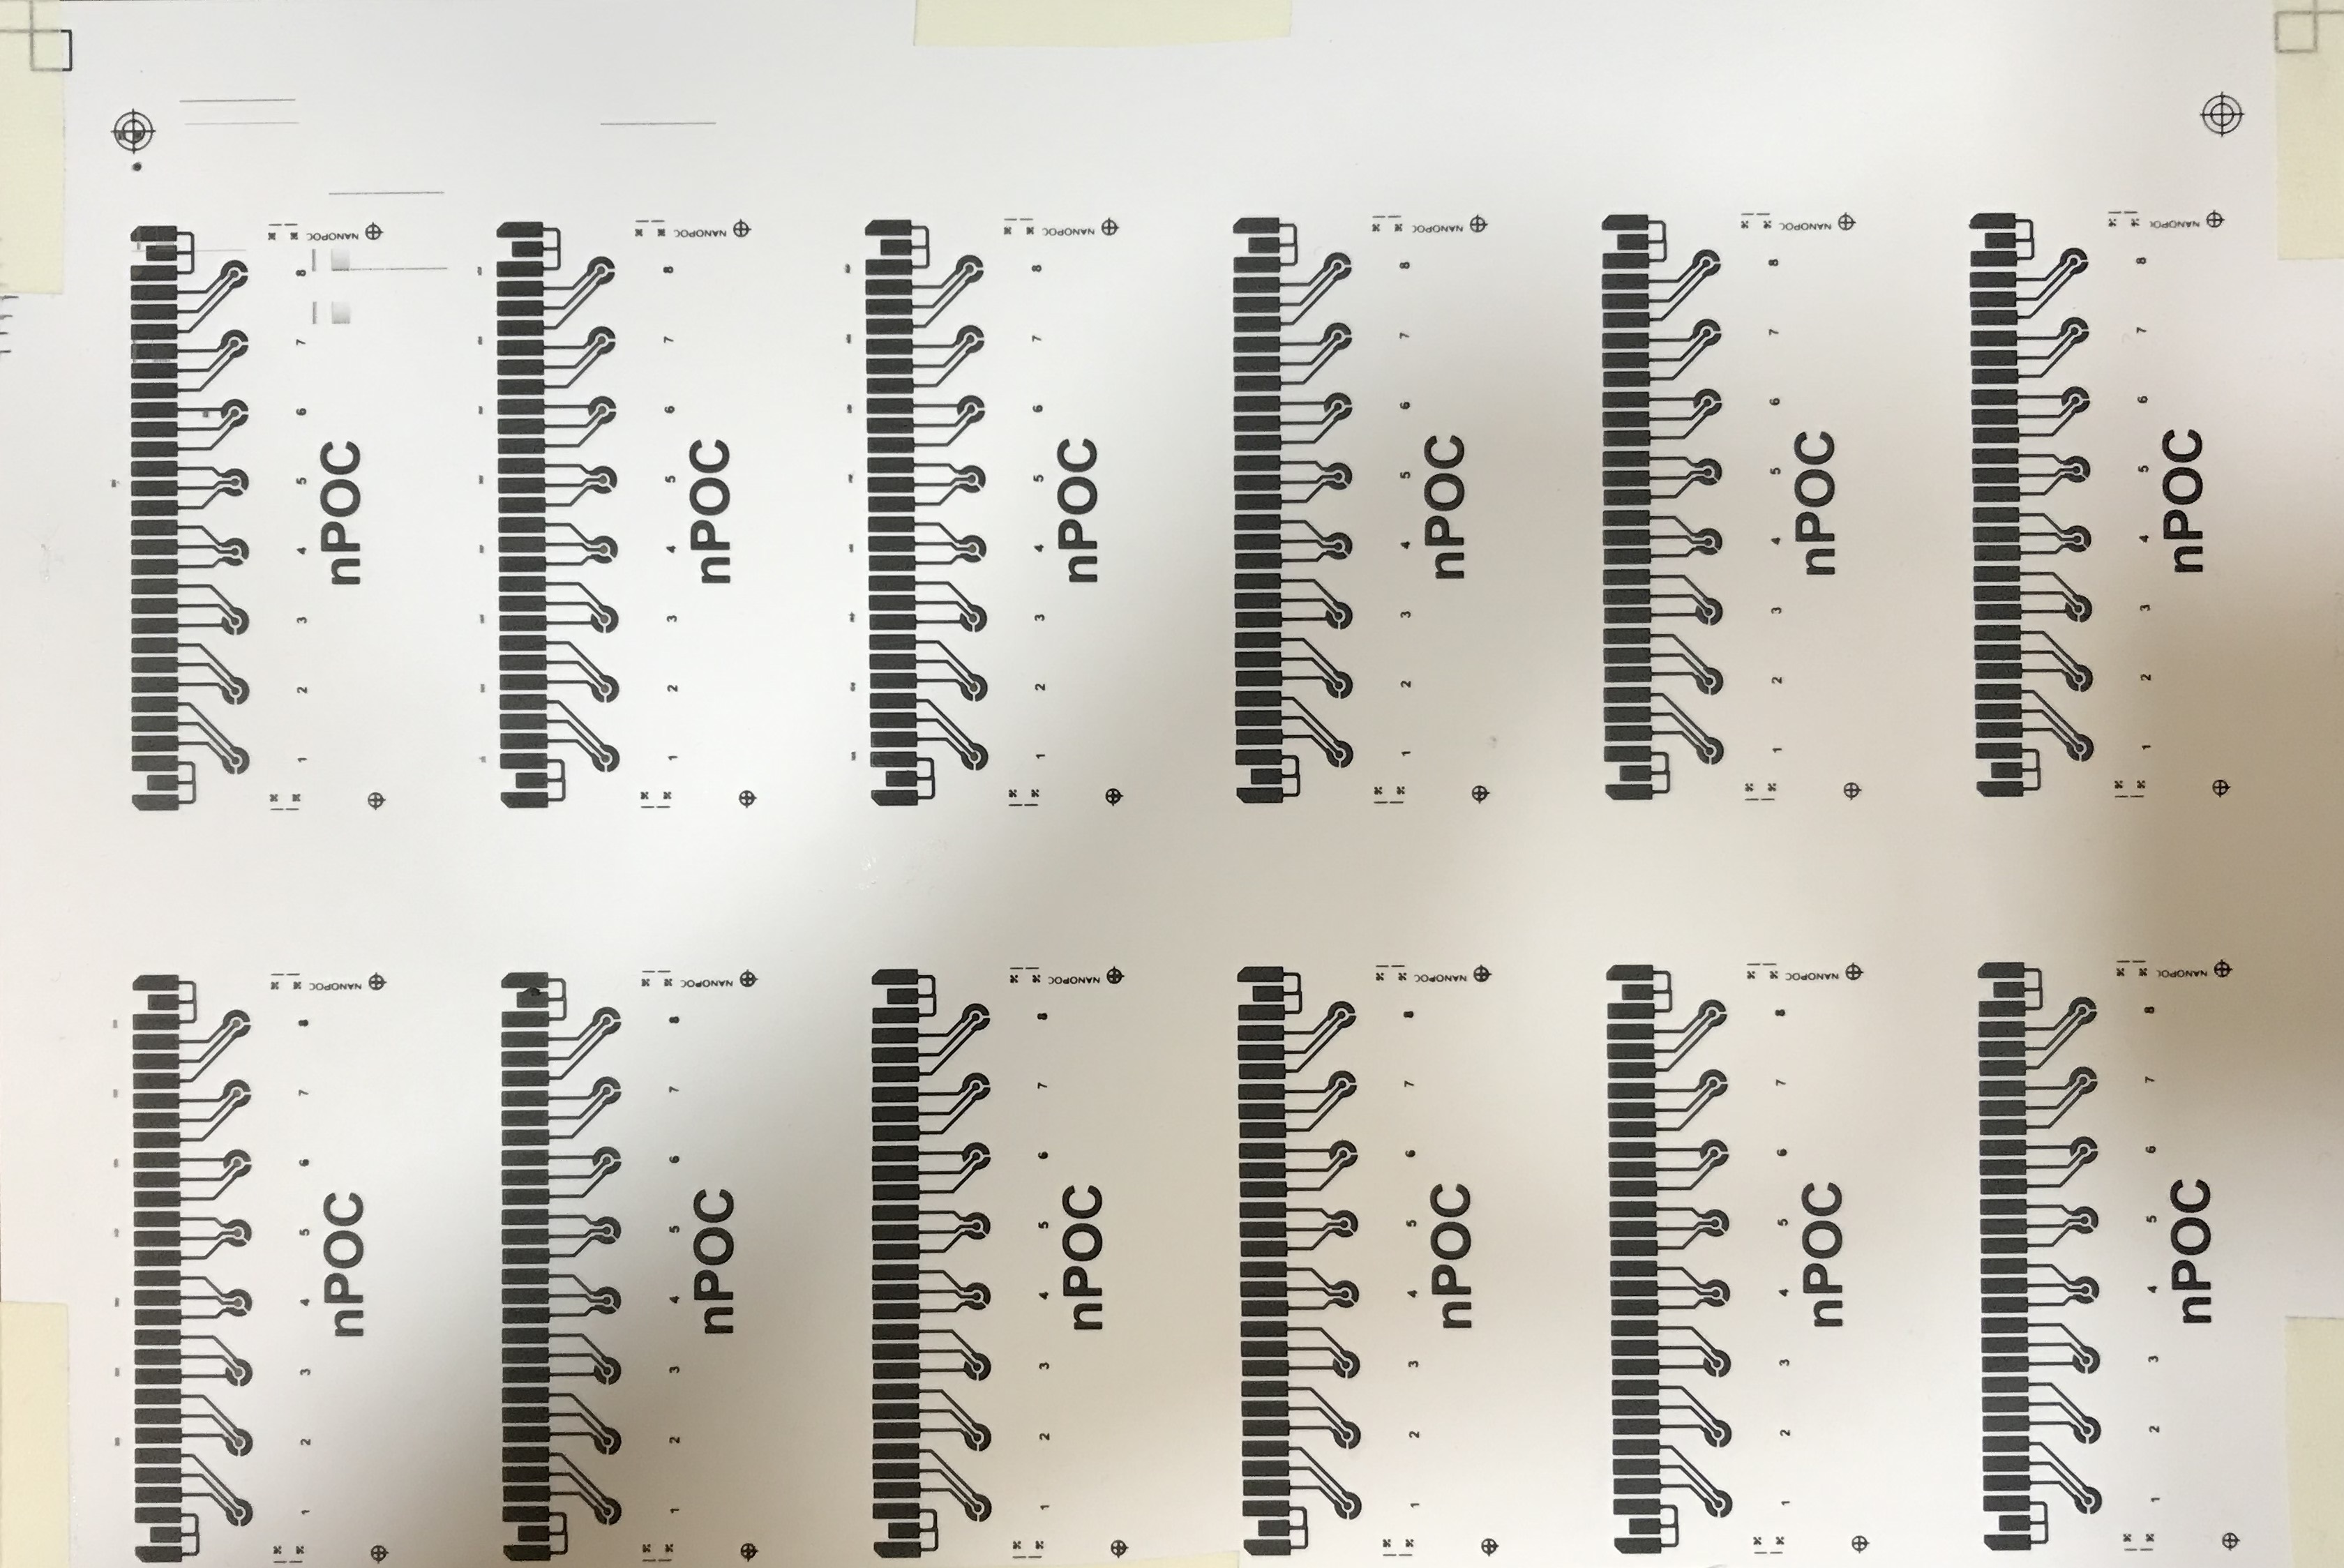
\includegraphics[width=0.5\textwidth]{Figuras/Figura_sensores_hoja_A4}
  \caption{Impresion serigráfica de biosensores en hoja A4}
  \label{fig:Figura_sensores_hoja_A4}
\end{figure}

\begin{figure}[H]
  \centering
    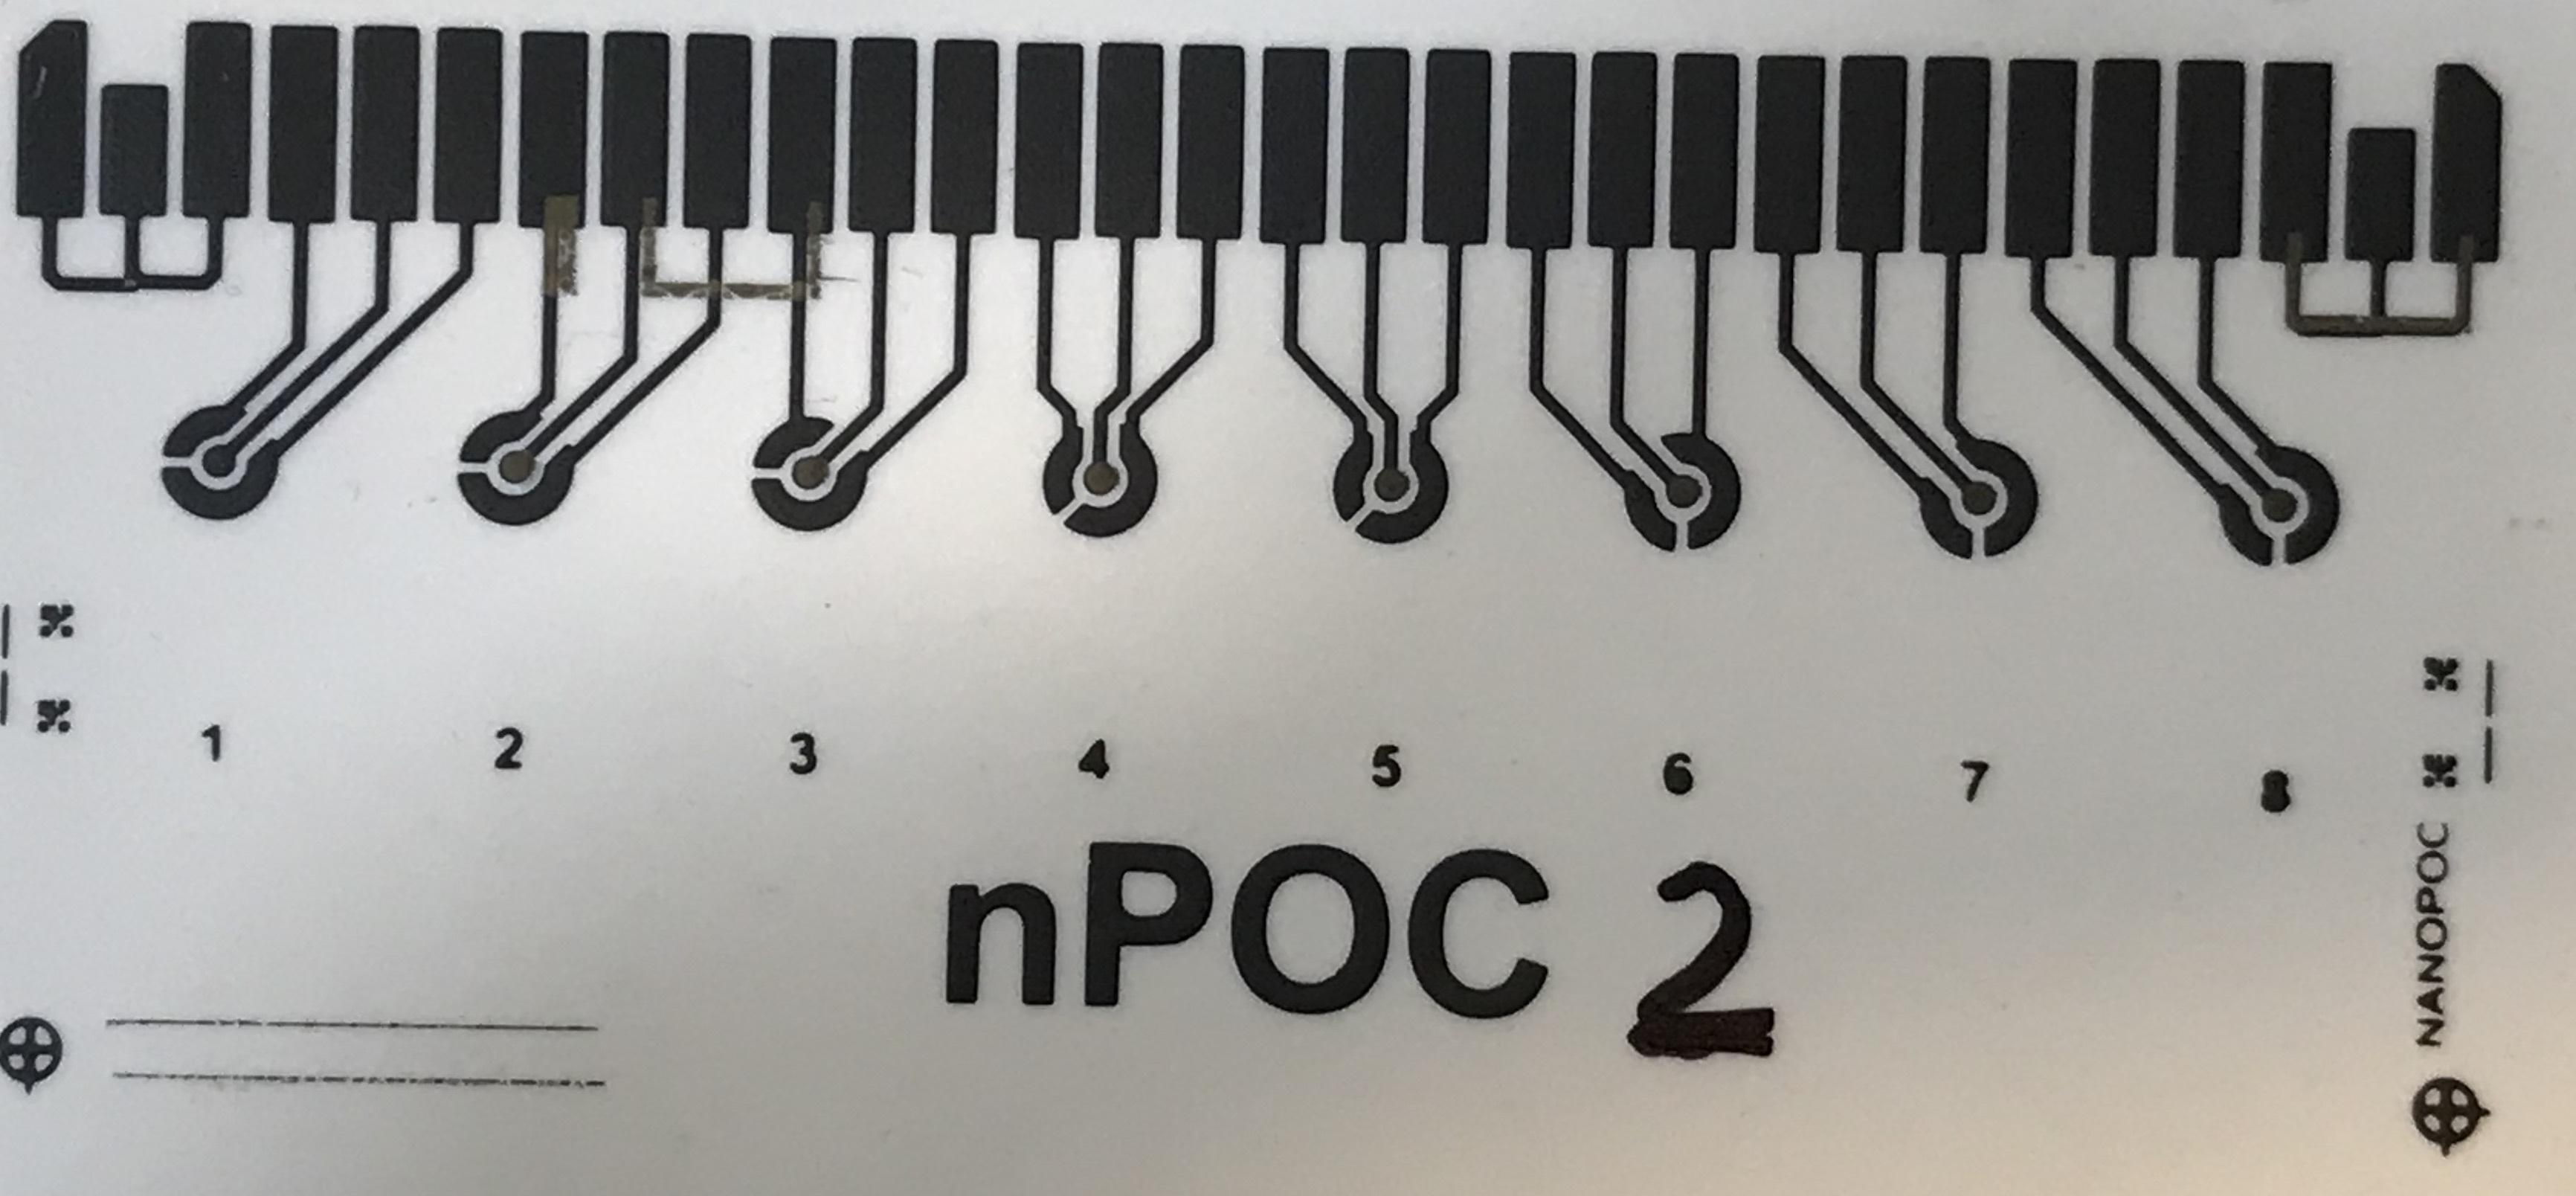
\includegraphics[width=0.5\textwidth]{Figuras/Figura_ejemplo_numeracion_nPoc}
  \caption{Ejemplo de numeración de sensor nPoc2}
  \label{fig:Figura_ejemplo_numeracion_nPoc}
\end{figure}

\subsection{Diseños de patrones de impresión}\label{subsec:diseno_impresion}
Una vez obtenidas las medidas necesarias de los sensores se procede a diseñar los patrones de impresión. Para esto se utilizó el editor profesional de vectores gráficos libre y de código abierto InkScape \cite{Inkscape} (Figura ~\ref{fig:Figura_Inkscape}).

\begin{figure}[H]
  \centering
    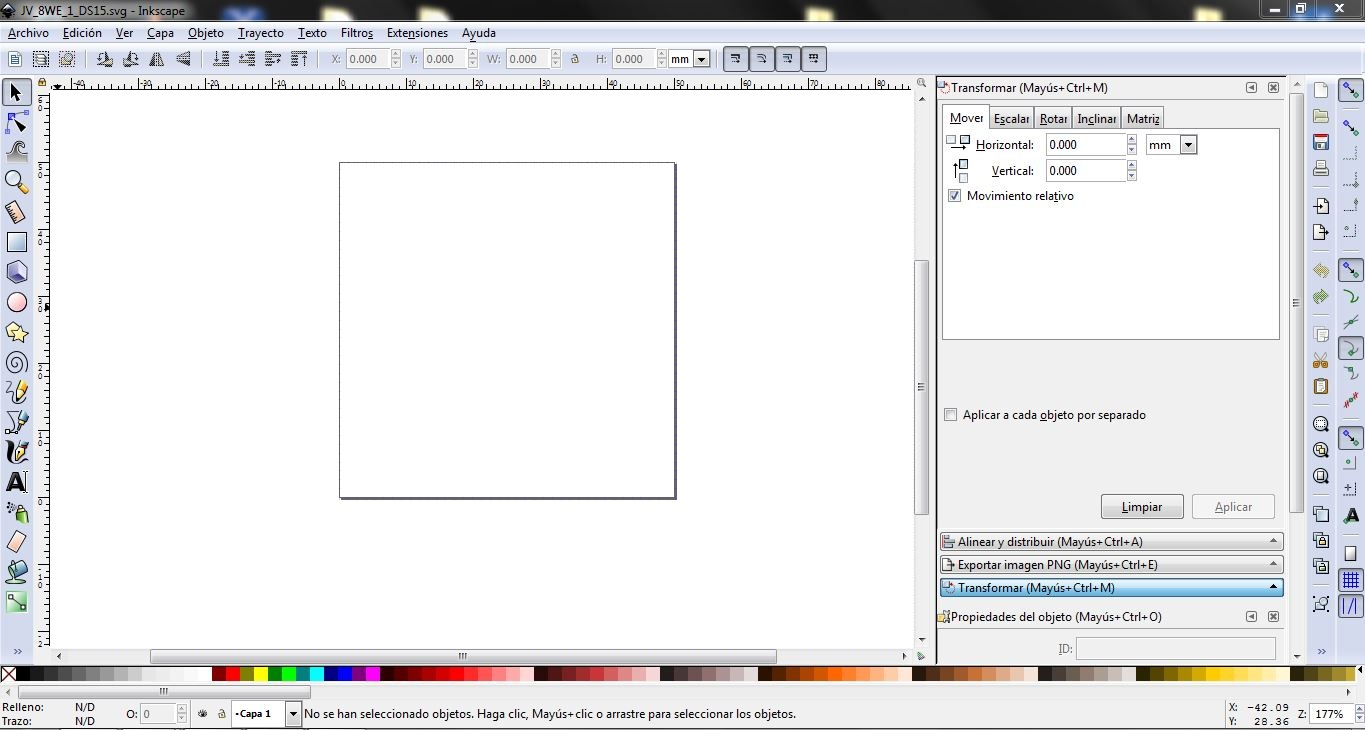
\includegraphics[width=0.65\textwidth]{Figuras/Figura_Inkscape}
  \caption{Editor profesional de vectores gráficos libre y de código abierto.}
  \label{fig:Figura_Inkscape}
\end{figure}

 Se realizaron cuatro dibujos con dos resoluciones posibles. Los primeros dibujos corresponden a un círculo de 1 mm y 1,1 mm de diámetro, el tamaño de un \emph{WE} y 100 $\mu$m más en el segundo. Con esto se pretende establecer si utilizando el mismo diámetro se logra una cobertura óptima con la tinta de nanopartículas de oro o se precisa agregar un \textit{offset}. Los otros dos dibujos constan de un arreglo de ocho círculos de 1 mm de diámetro, espaciados 9 mm entre sí y un arreglo de ocho círculos de 1,1 mm de diámetro, con el mismo espaciado (Figura ~\ref{fig:Figura_Diseno_Circulos}). Las resoluciones utilizadas fueron de 1693.33 y 1270 dpi, posteriormente se explicará la razón de dichas resoluciones.

\begin{figure}[H]
  \centering
    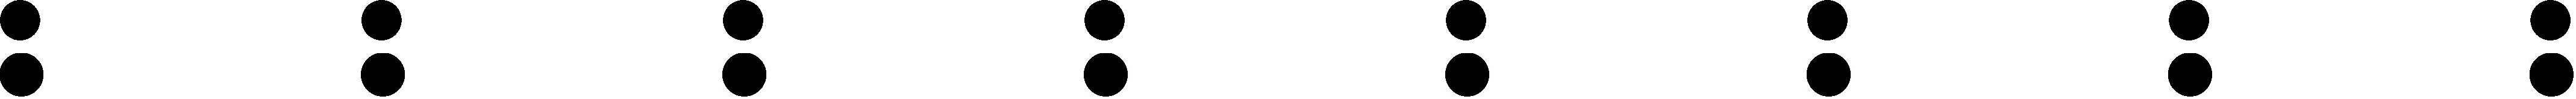
\includegraphics[width=0.5\textwidth]{Figuras/Figura_Diseno_Circulos}
  \caption{Diseños de impresiones en 1 y 1,1 mm.}
  \label{fig:Figura_Diseno_Circulos}
\end{figure}

Dado que el software de la impresora (\textit{Dimatix Drop Manager}) no detecta imágenes a color o a escala de grises, se deben convertir las imágenes en archivos de 1 bit monocromático. De esta forma lo único presente en la imagen son pixeles blancos o negros, correspondiendo a donde debe eyectarse o no una gota de tinta. El formato que puede guardar imágenes de 1 bit es el Windows bitmap (ó BMP por sus siglas en inglés), y por esto es el único formato externo soportado por el \textit{Dimatix Drop Manager}. La conversión a formato BMP se realiza mediante el Software \textit{Microsoft Paint}. Realizando un zoom sobre la misma imagen en formato PNG y BMP, se pueden apreciar las diferencias a simple vista (Figura ~\ref{fig:Figura_comparacion_png_bmp}).

\begin{figure}[H]
  \centering
    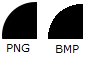
\includegraphics[width=0.5\textwidth]{Figuras/Figura_comparacion_png_bmp}
  \caption{Comparación archivos PNG y BMP.}
  \label{fig:Figura_comparacion_png_bmp}
\end{figure}

Una vez obtenidos los archivos en el formato correcto se puede proceder a la preparación y puesta a punto de los parámetros de la impresora.


\section{Puesta a punto y calibraci\'on de impresora}\label{sec:calib_impresora}
Luego de preparar, colocar y configurar el cartucho de tinta y el sustrato (ver \hyperref[chap:apendiceA]{Anexo A}) se debe agregar el diseño o patrón que se quiere imprimir.

Para esto el software DMP ofrece dos opciones. La primera permite realizar el dibujo con el mismo programa agregando posiciones (coordenadas X e Y) y los espesores deseados; la segunda permite importar imágenes con formato BMP monocromático. La creación de diseños mediante el software de DMP solo permite formas básicas y sobre todo confomadas por líneas rectas. Para dibujos más complejos se recomienda el procedimiento de diseño externo explicado en el apartado de diseño de patrones de impresión (Capítulo 3, \hyperref[subsec:diseno_impresion]{apartado 3.1.2}).

Para cualquiera de las dos opciones se les puede agregar coordenadas de referencia, utilizadas para ubicar la impresión en el sustrato y un $``$\textit{Leader Bar}$"$ con la posibilidad de configurar su ancho y su distancia ($``$\textit{Gap}$"$) con el diseño a imprimir. Esta última función es un procedimiento comúnmente utilizado para mantener los inyectores activos y su velocidad de caída uniforme al momento de la impresión, mejorando la calidad del patrón. Se debe tener en consideración que los $``$\textit{Leader Bars}$"$ deben ubicarse dentro del sustrato, de lo contrario se estará eyectando tinta sobre la platina de la impresora (Figura ~\ref{fig:Figura_Leader_Bar}).

\begin{figure}[H]
  \centering
    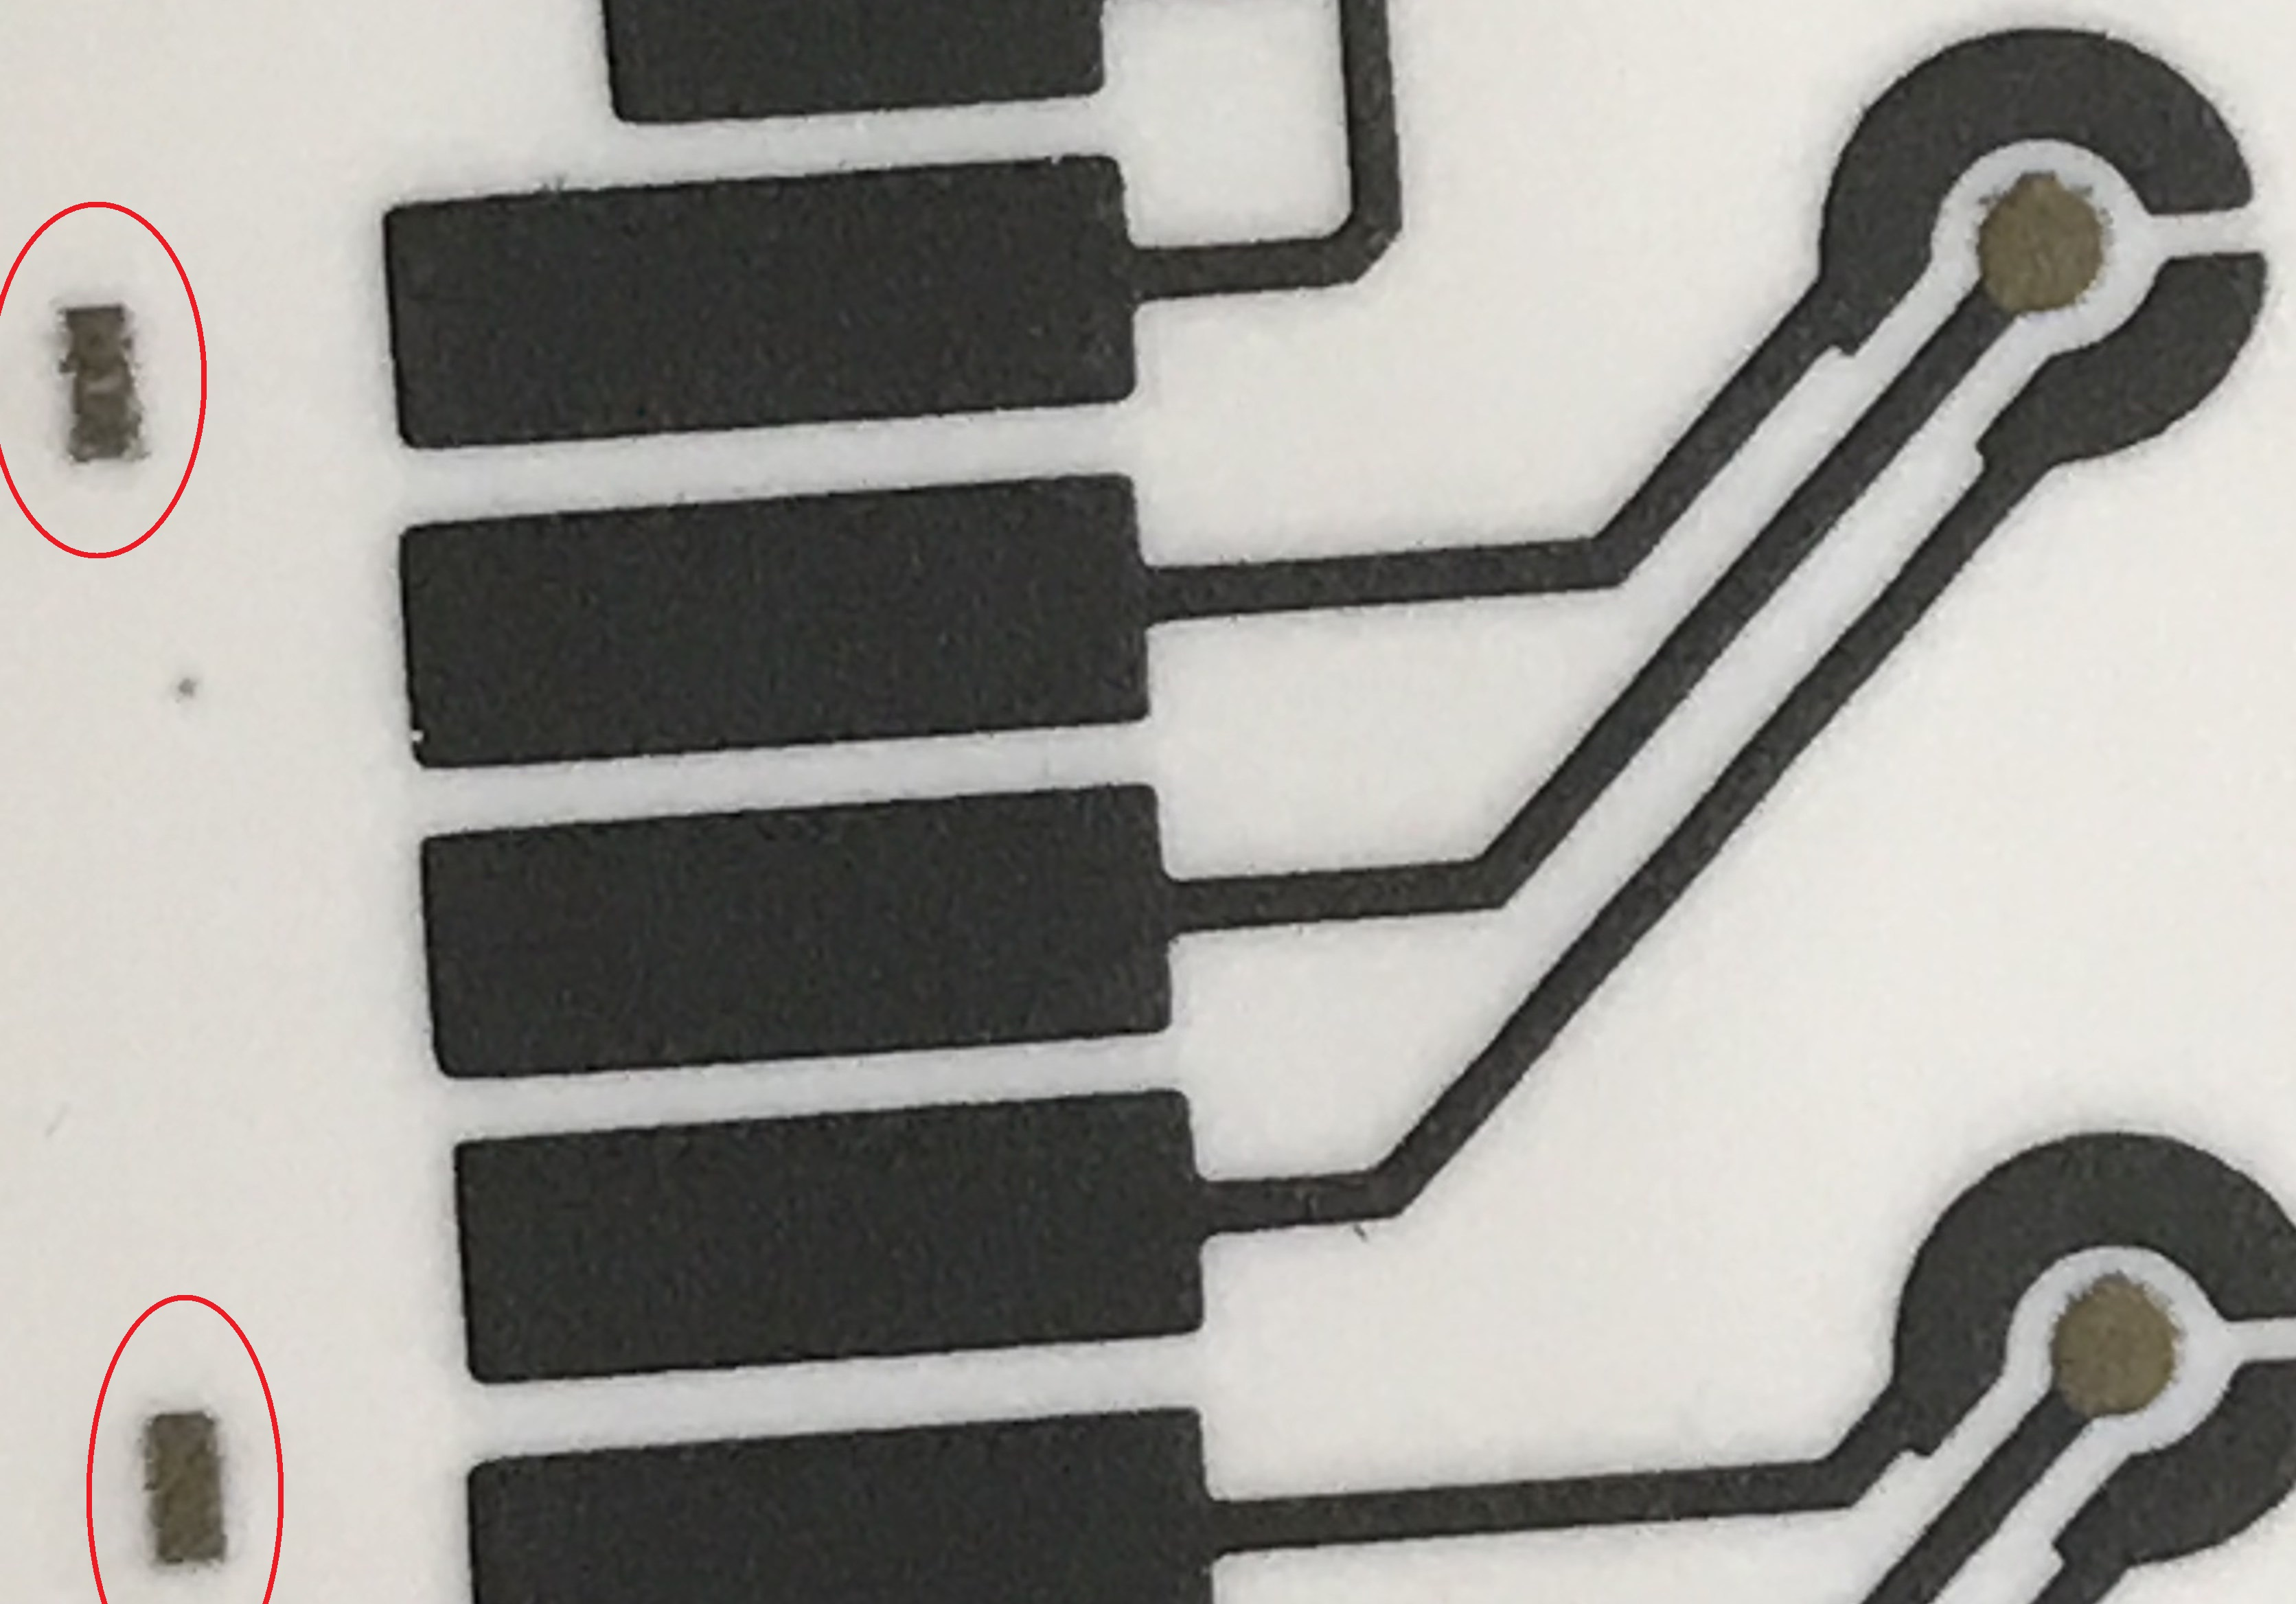
\includegraphics[width=0.5\textwidth]{Figuras/Figura_Leader_Bar}
  \caption{$``$\textit{Leader Bars}$"$ impresos sobre sustrato.}
  \label{fig:Figura_Leader_Bar}
\end{figure}

Llegado este momento, si no se realizó anteriormente, es aconsejable calibrar las tensiones de eyección de los inyectores (del inglés $``$\textit{Nozzles}$"$) que serán utilizados mediante el $``$\textit{Drop Watcher}$"$ (Figura ~\ref{fig:Figura_nozzles}). Este sistema consta de una cámara orientada a 45º del plano horizontal con foco en los eyectores del cabezal que ,mediante una luz estroboscópica, permite realizar fotografías o filmaciones sobre el funcionamiento de los orificios del cabezal (Eyección de gotas).

\begin{figure}[H]
  \centering
    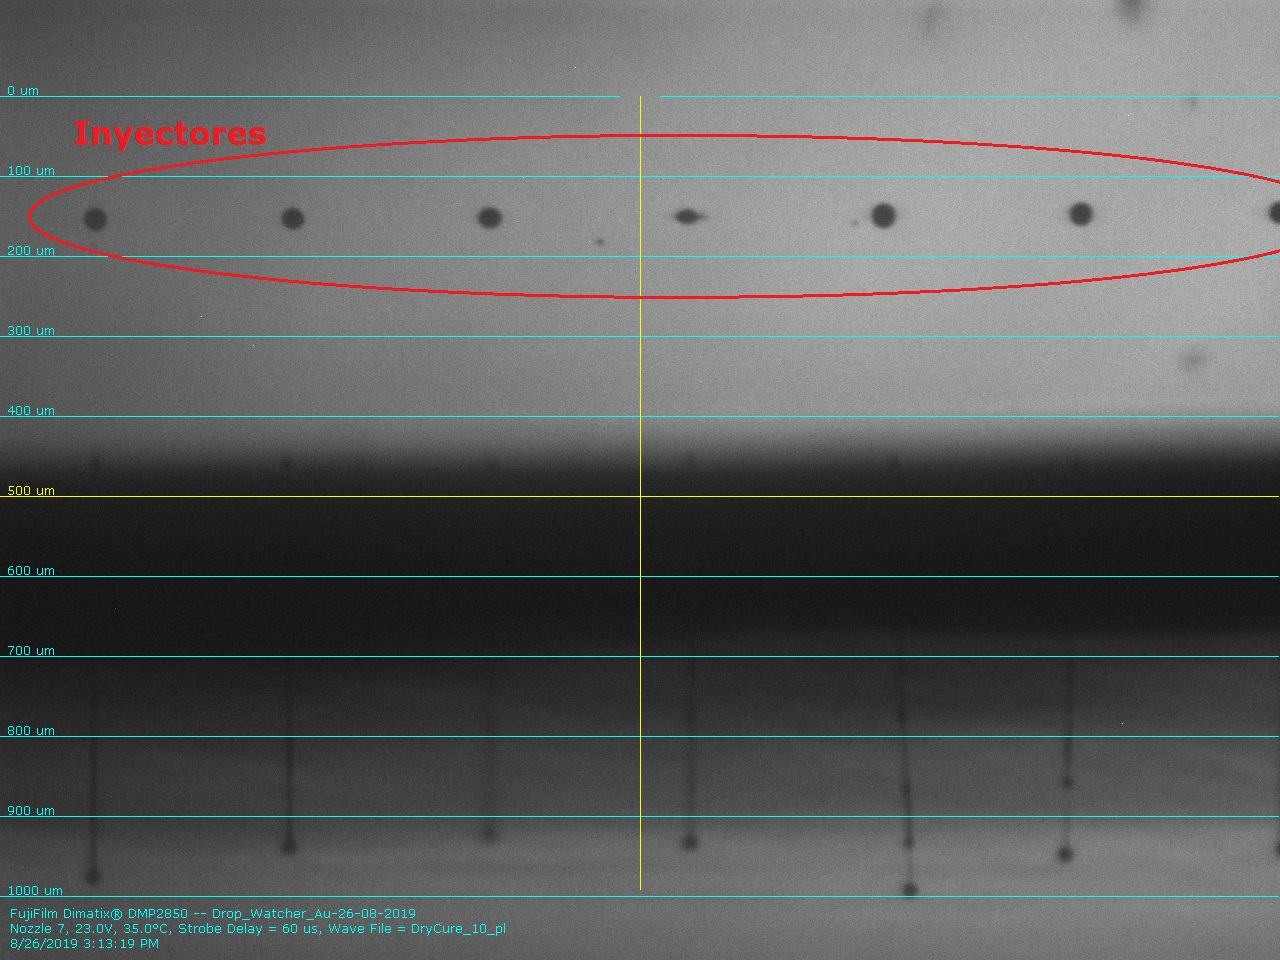
\includegraphics[width=0.5\textwidth]{Figuras/Figura_nozzles}
  \caption{Inyectores vistos desde cámara $``$\textit{Drop Watcher}$"$.}
  \label{fig:Figura_nozzles}
\end{figure}

Luego, utilizando la cámara fiducial, se realizan los procesos de alineación de gotas, sustrato y se fijan las coordenadas donde comienza la impresión.

La alineación del sustrato se logra mediante la calibración de \textit{Theta}. Para este procedimiento se deben seleccionar dos puntos que se encuentren alineados sobre el sustrato. En este caso, la impresión de carbono incluye distintos puntos de alineación, utilizando los más pequeños para obtener una mayor precisión, minimizando el error por el ancho mínimo de impresión de la fabricación serigráfica (Figura ~\ref{fig:Figura_alineacion_theta}).

\begin{figure}[H]
  \centering
    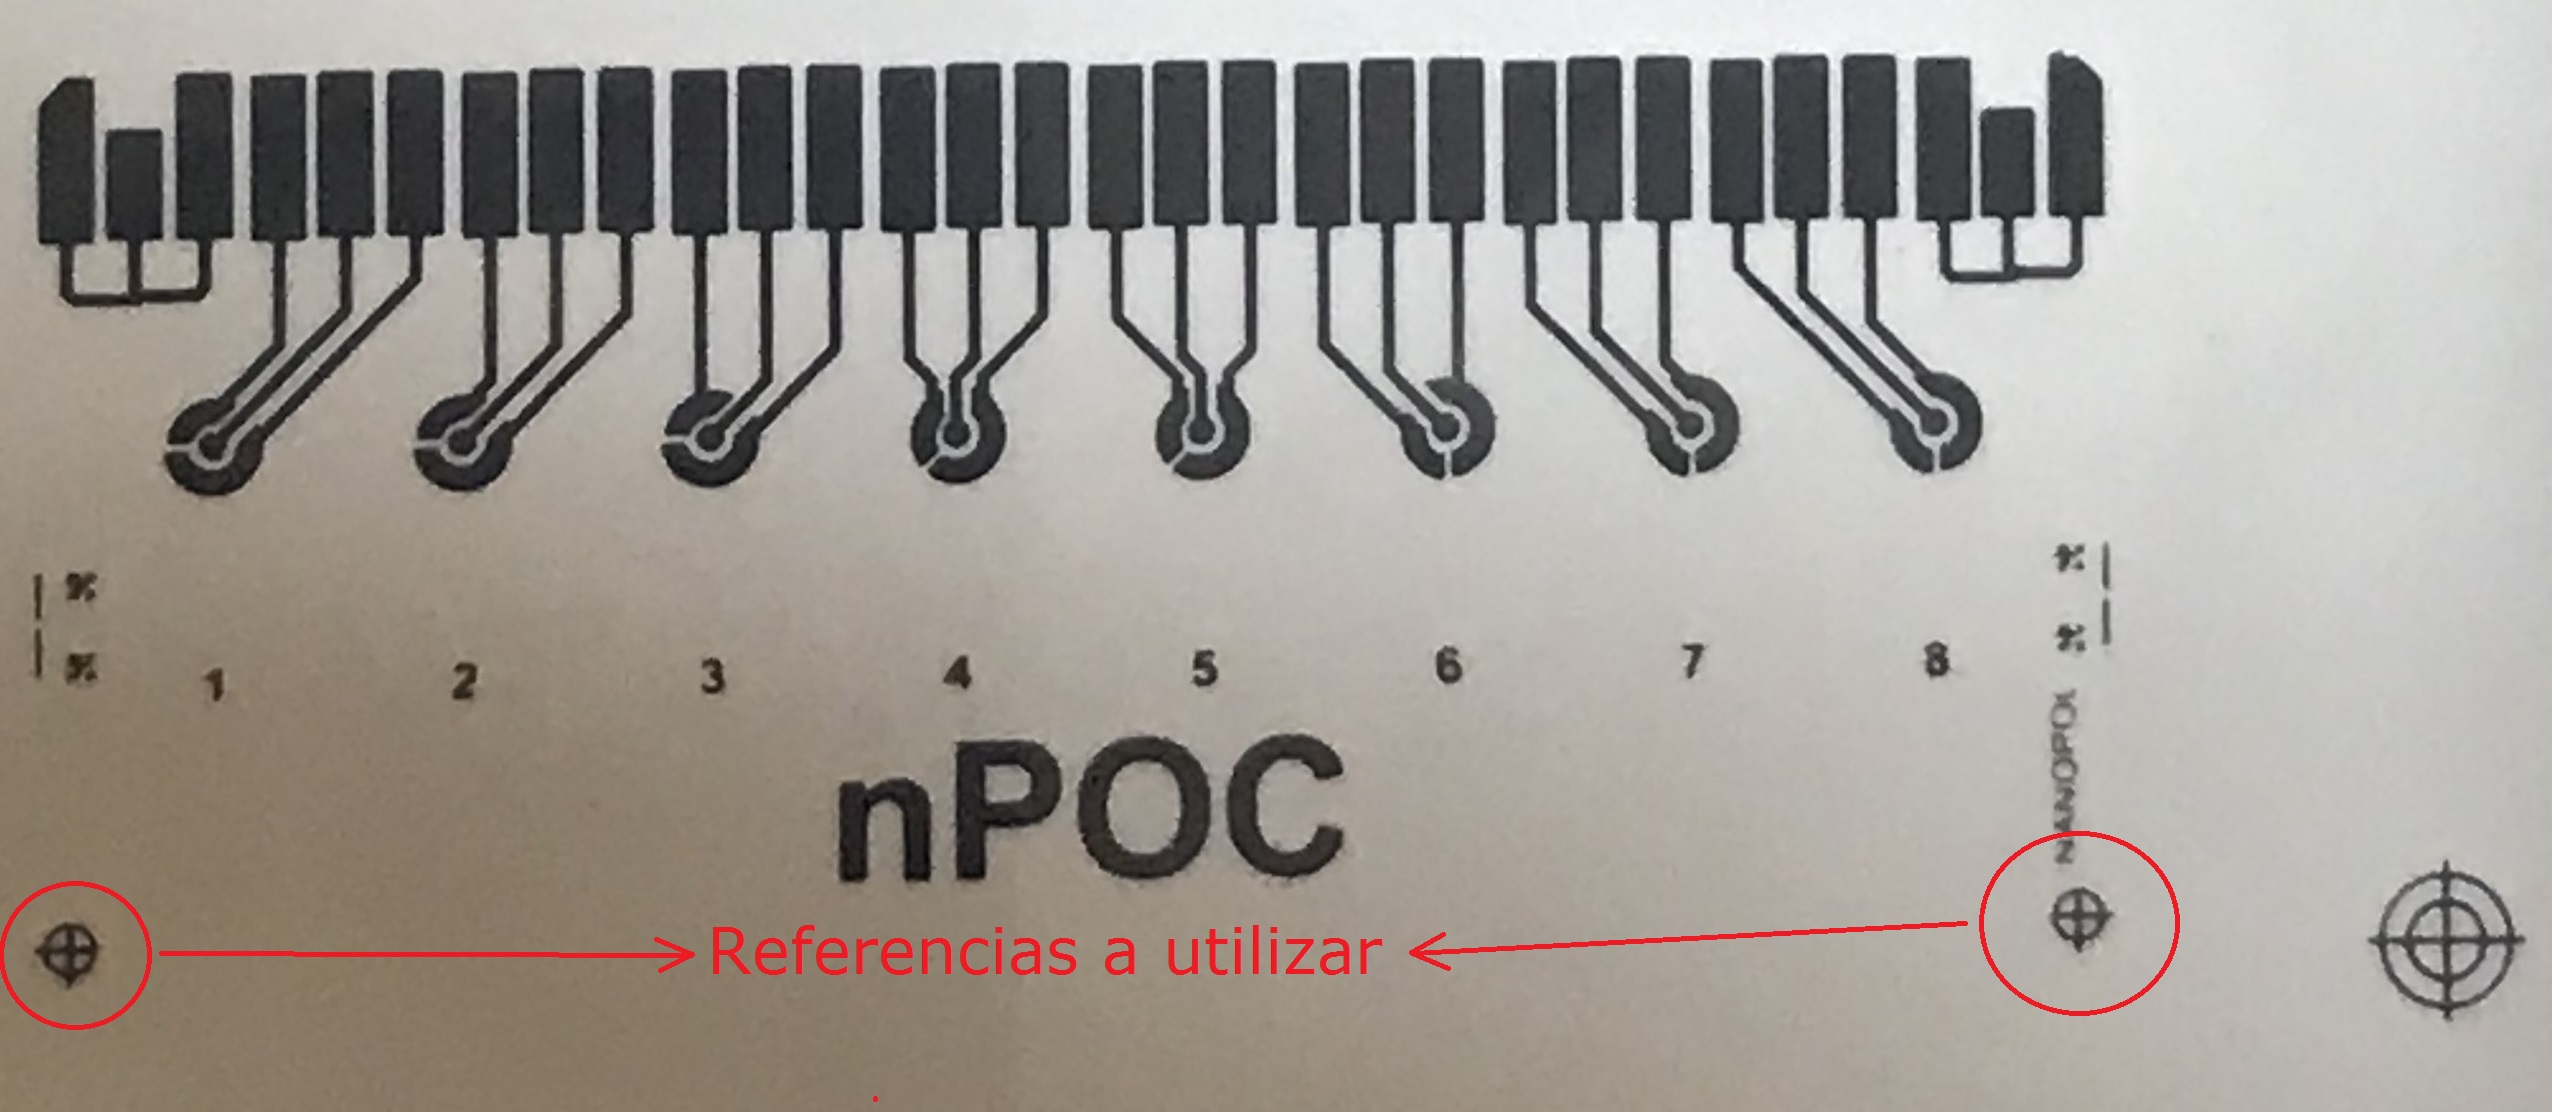
\includegraphics[width=0.5\textwidth]{Figuras/Figura_alineacion_theta}
  \caption{Referencias a utilizar para la calibración de \textit{Theta}.}
  \label{fig:Figura_alineacion_theta}
\end{figure}

Si bien, a simple vista, los objetos de alineación parecen de trazos finos y regulares, al utilizar la cámara fiducial se ve que no es sencillo determinar el punto medio (Figura ~\ref{fig:Figura_alineacion_theta2}).

\begin{figure}[H]
  \centering
    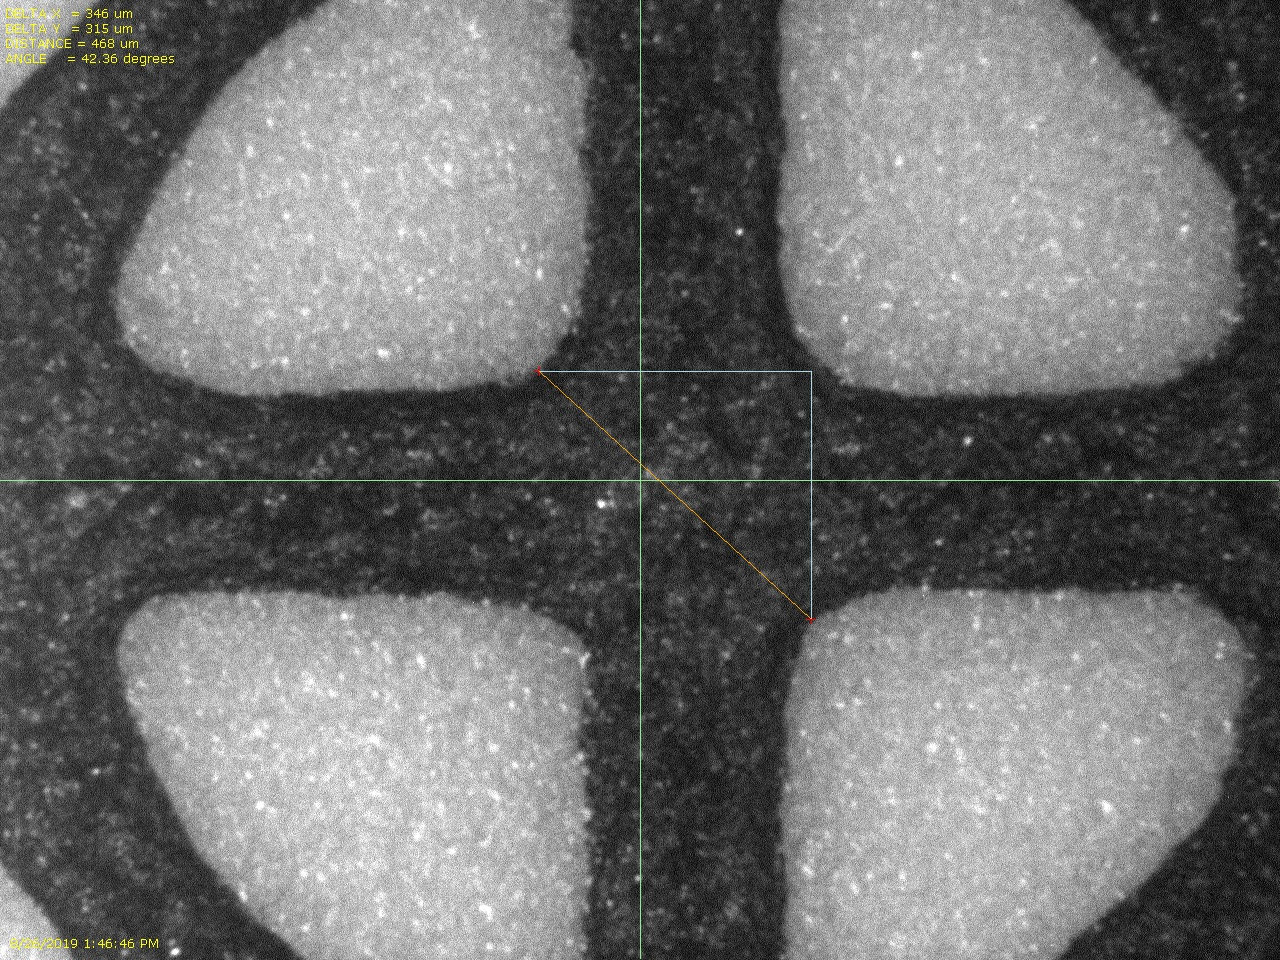
\includegraphics[width=0.4\textwidth]{Figuras/Figura_alineacion_theta2}
  \caption{Objeto de alineación visto con cámara fiducial.}
  \label{fig:Figura_alineacion_theta2}
\end{figure}

Seguido a alinear el sustrato, se debe definir el espaciado entre gotas que se utilizará al imprimir. Este parámetro es identificado como $``$\textit{Drop Spacing}$"$ (Desde ahora \emph{DS}) y, para determinarlo, se utilizó un patrón de gotas con los diferentes espaciados permitidos por la impresora, llamado $``$\textit{Line Pattern}$"$(Figura ~\ref{fig:Figura_Line_Pattern_Micro50X}). Luego de imprimir, se decide que $``$\textit{Drop Spacing}$"$ genera la línea mejor definida, tanto en continuidad como en homogeneidad de ancho de línea y espesor, sobre el sustrato a utilizar. Para la tinta de oro sobre \textit{Valox} se decidió utilizar un espaciado de 15 $\mu$m entre gotas, dado que este muestra una línea continua sin generar $``$\textit{Clusters}$"$ de tinta.

\begin{figure}[H]
  \centering
    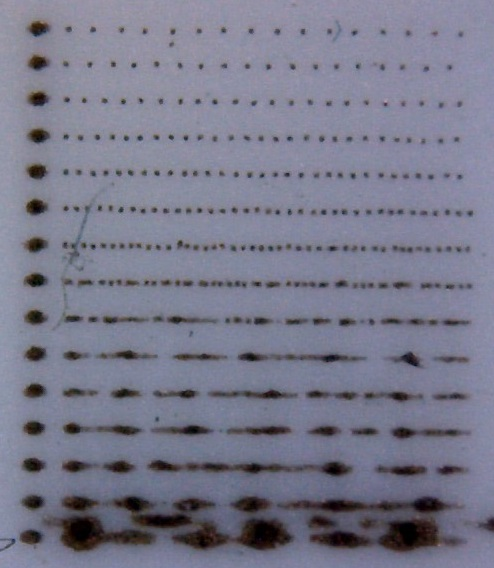
\includegraphics[width=0.35\textwidth]{Figuras/Figura_Line_Pattern_Micro50X}
  \caption{$``$\textit{Line Pattern}$"$, vista con microscopio de 50X.}
  \label{fig:Figura_Line_Pattern_Micro50X}
\end{figure}

Una vez definido el \emph{DS}, se ajusta la resolución del diseño que se desea imprimir. En el caso del $``$\textit{Drop Spacing}$"$ de 15 $\mu$m entre gotas, se utiliza una resolución de 1693.33 puntos por pulgada ($``$\textit{dpi}$"$). El manual de instrucciones de la impresora \cite{DimatixUM} brinda una tabla con la resolución que debe tener el diseño y el ángulo al que debe configurarse el cartucho para cada \emph{DS} (Figura ~\ref{fig:Figura_Tabla_angulos}).

\begin{figure}[H]
  \centering
    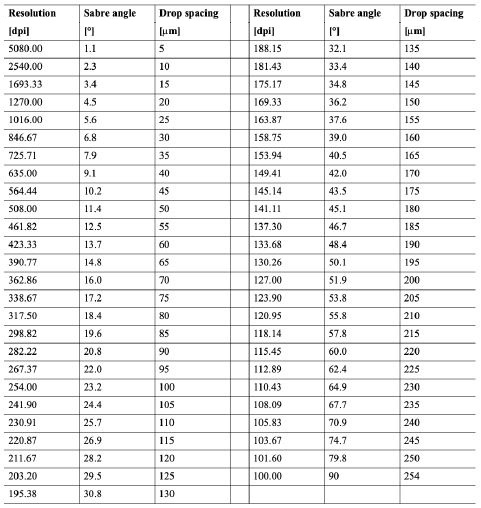
\includegraphics[width=0.5\textwidth]{Figuras/Figura_Tabla_angulos}
  \caption{Tabla de resoluciones y ángulos para cada \emph{DS}.}
  \label{fig:Figura_Tabla_angulos}
\end{figure}

A continuación se debe realizar la calibración de $``$\textit{Drop Offset}$"$. Este procedimiento compensa el error entre el punto en que la cámara fiducial está captando y la posición en la que el cartucho está imprimiendo. Es decir, compensa el vuelo de las gotas de tinta entre su eyección del cabezal hasta su impacto con el sustrato. Para esto, la impresora realiza una línea continua de 10 mm en el eje X seguido de un punto a 1 mm de la línea. La calibración se realiza una vez que se ubica este punto en la cámara fiducial y se hace $``$\textit{click}$"$ sobre él, lo más centrado posible (Figura ~\ref{fig:Figura_prueba_Drop_Spacing}).

\begin{figure}[H]
  \centering
    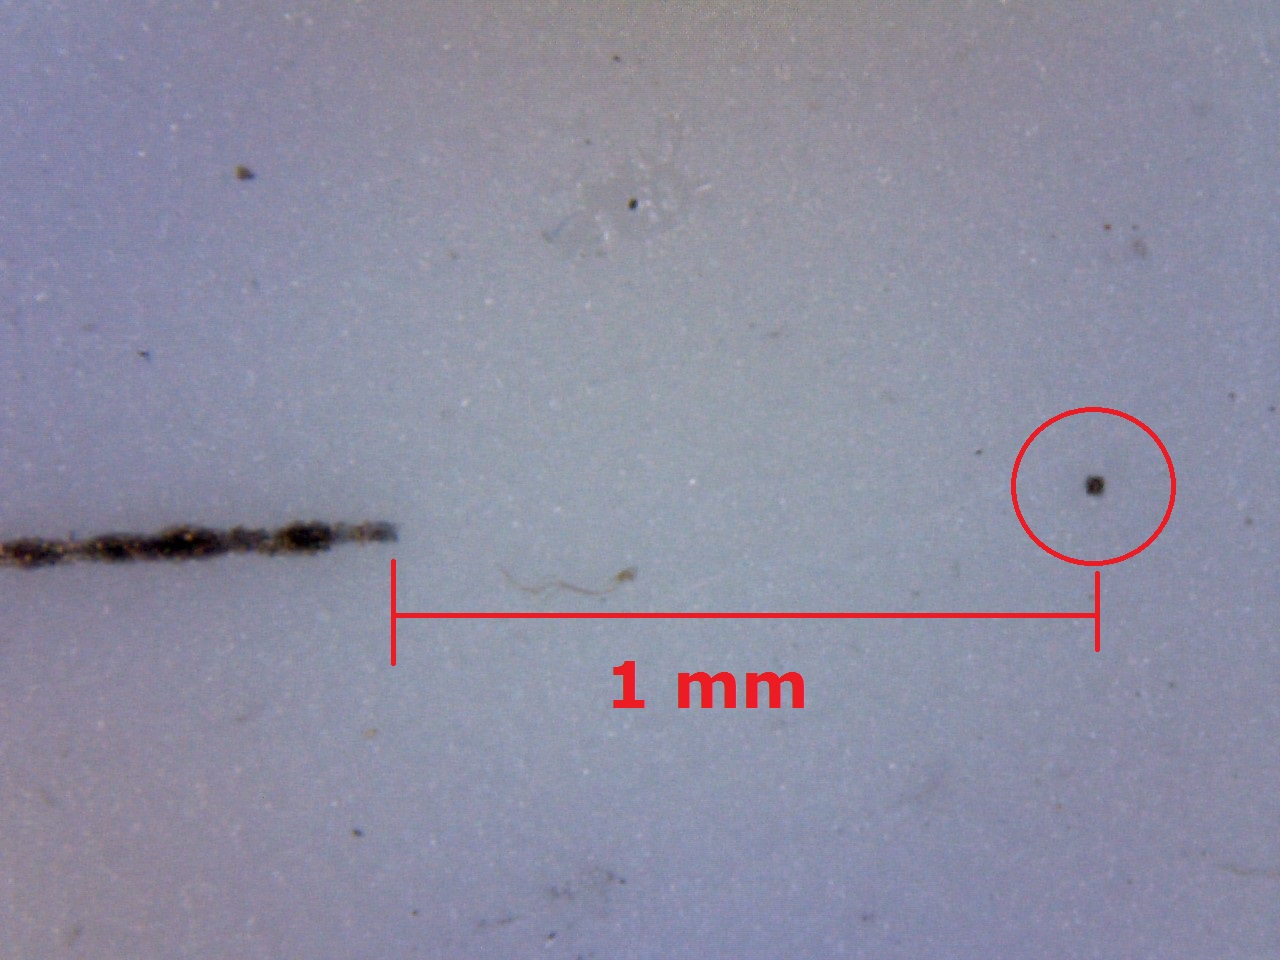
\includegraphics[width=0.5\textwidth]{Figuras/Figura_prueba_Drop_Spacing}
  \caption{Fin de línea y punto de procedimiento $``$\textit{Drop Offset}$"$, vista con microscopio de 1000X.}
  \label{fig:Figura_prueba_Drop_Spacing}
\end{figure}

La cámara fiducial es un elemento que forma parte del carrete donde se coloca el cartucho (Figura ~\ref{fig:Figura_Camara_Fiducial}). Esta es utilizada para los procedimientos de alineación del sustrato,  la calibración del tiempo de vuelo de las gotas eyectadas, el chequeo del sustrato y las impresiones sobre el mismo o mediciones sobre la superficie colocada sobre la platina. Tiene un campo de visión de 1,62 mm de ancho y 1,22 mm de alto, con una resolución de 2,54 $\mu$m por pixel.

\begin{figure}[H]
  \centering
    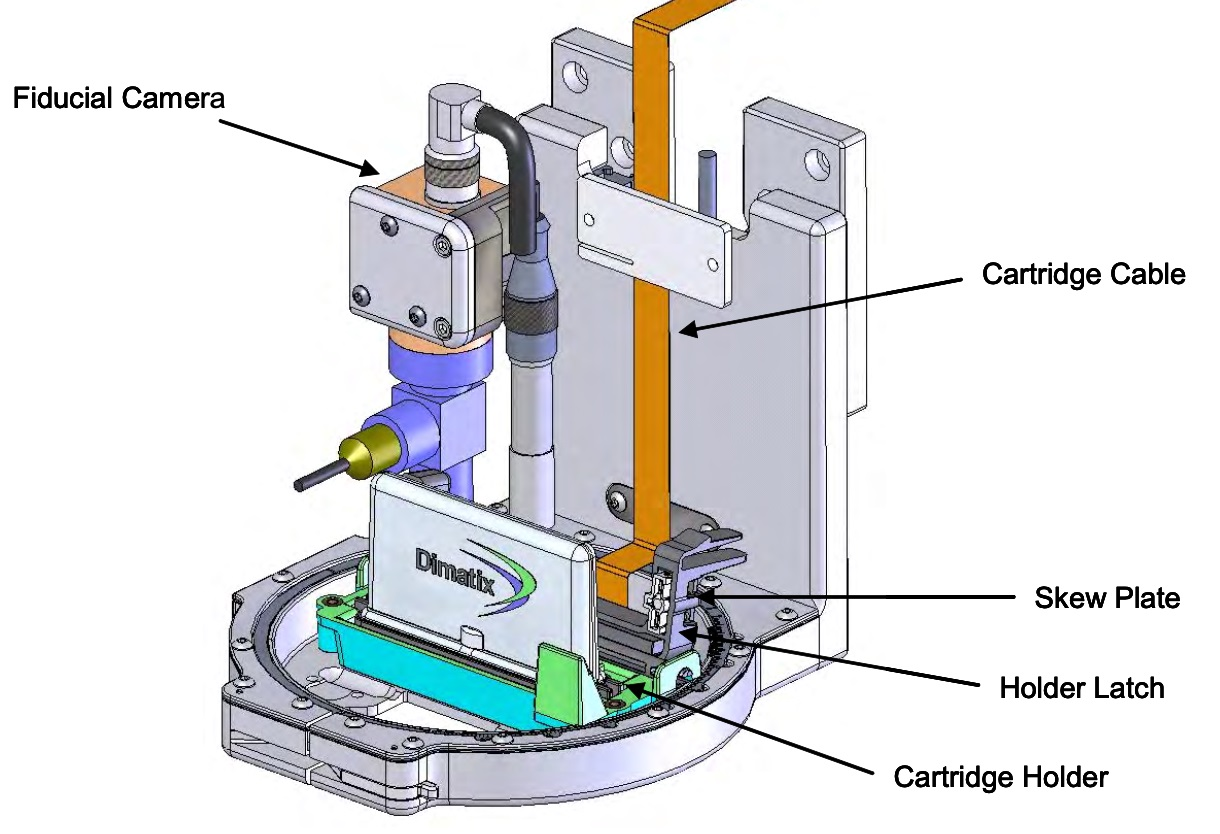
\includegraphics[width=0.5\textwidth]{Figuras/Figura_Camara_Fiducial}
  \caption{Ilustración de los distintos componentes del carrete de la impresora.}
  \label{fig:Figura_Camara_Fiducial}
\end{figure}

Como última configuración antes de comenzar la impresión, se deben definir las coordenadas del sustrato donde se comenzará a imprimir ($``$\textit{Print Origin}$"$) o de referencia, que concordarán con las definidas en el diseño ($``$\textit{Reference Point}$"$).

Si se decide utilizar el punto donde se comenzará a imprimir, se debe elegir la función \textit{Set Print Origin} de la cámara fiducial. En cambio, si se desea referenciar un punto del diseño con el sustrato, debe configurarse la función \textit{Set Reference Point} (Figura ~\ref{fig:Figura_Ventana_Camara_Fiducial}). Al utilizar la última función debe tenerse en cuenta que el punto de referencia debe estar definido en el diseño antes de cargarlo en la solapa de imagen a imprimir del software \textit{DMP}.

\begin{figure}[H]
  \centering
    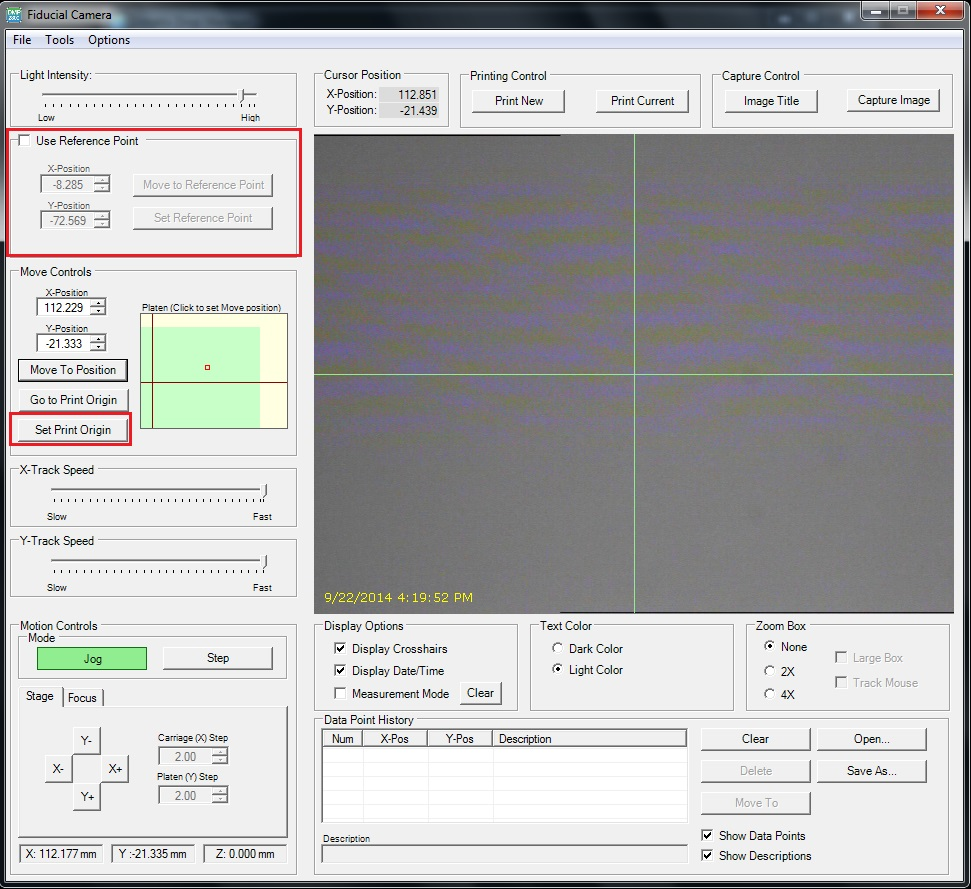
\includegraphics[width=0.5\textwidth]{Figuras/Figura_Ventana_Camara_Fiducial}
  \caption{Ventana de cámara fiducial con opciones para \textit{Print Origin} y \textit{Reference Point}.}
  \label{fig:Figura_Ventana_Camara_Fiducial}
\end{figure}

Para este trabajo se decidió utilizar como punto de referencia el centro del primer círculo, alineándolo con el electrodo de trabajo 1 del sensor. De esta manera, los otros 7 círculos quedaron alineados con su respectivo electrodo.

\section{Impresiones}
Como primera prueba, se realizó la impresión de un círculo de 1 mm de diámetro sobre la tinta de carbono y sobre el sustrato \textit{Valox}, para verificar el comportamiento de la tinta de oro sobre ambas superficies (Figura ~\ref{fig:Figura_Prueba_Sobre_Sustratos}).

\begin{figure}[H]
  \centering
    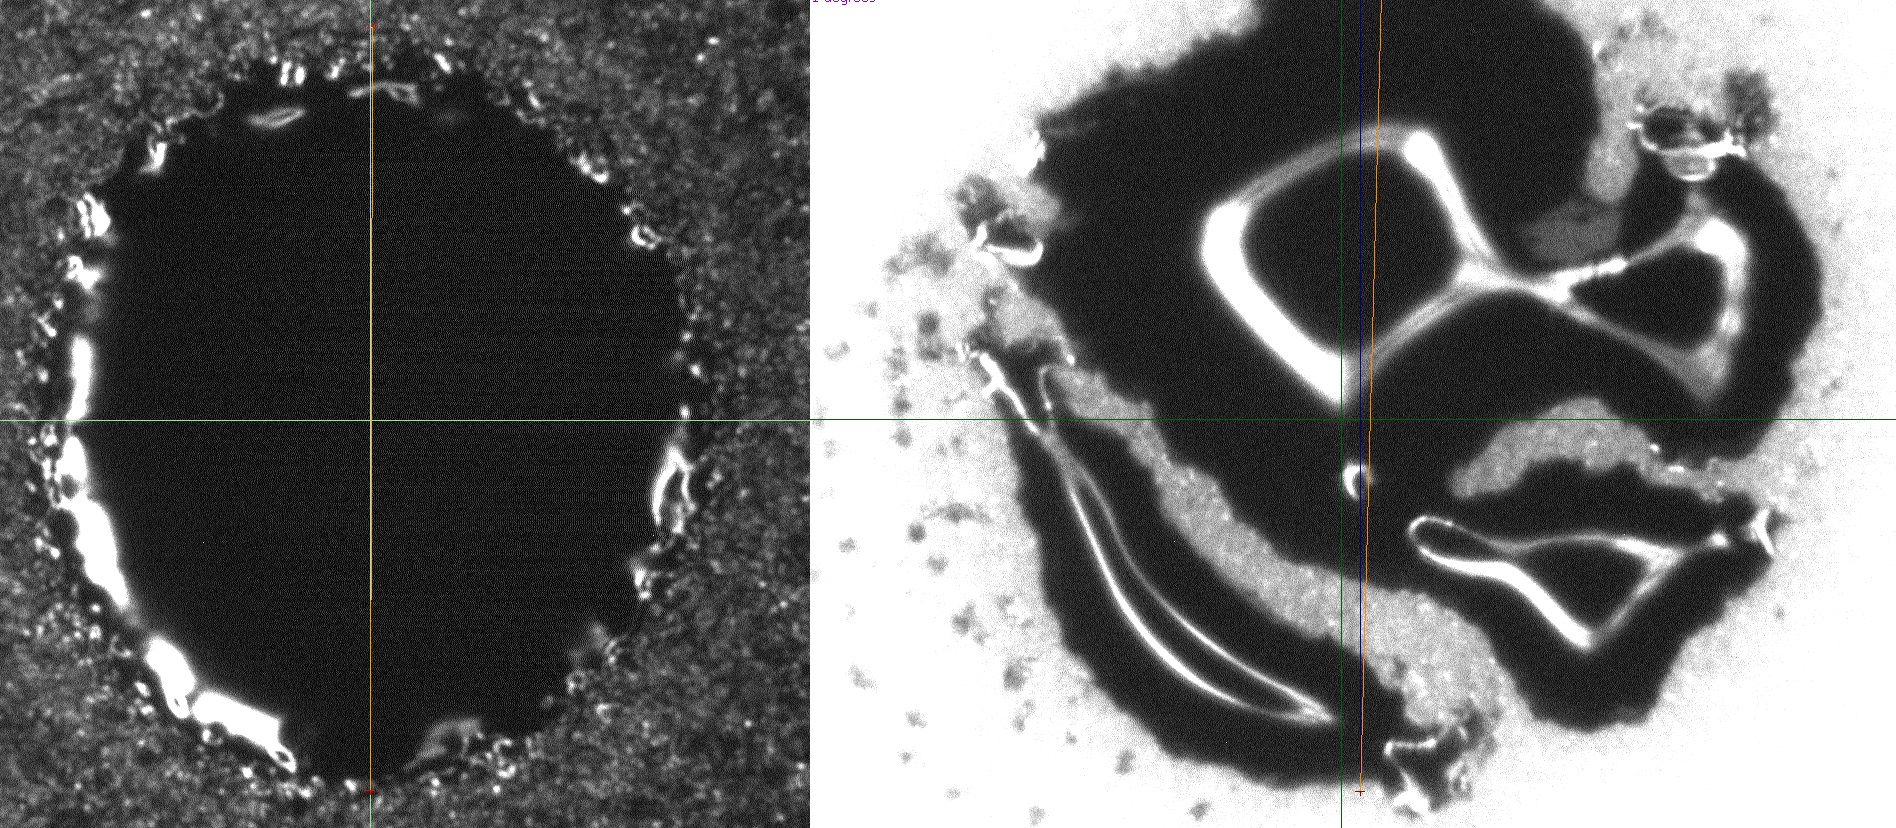
\includegraphics[width=0.5\textwidth]{Figuras/Figura_Prueba_Sobre_Sustratos}
  \caption{Prueba tinta de oro sobre tinta de carbono y sustrato \textit{Valox}.}
  \label{fig:Figura_Prueba_Sobre_Sustratos}
\end{figure}
Como se esperaba, la tinta de oro muestra un mejor anclaje sobre el carbono que sobre el sustrato.

La siguiente prueba fue alinear el punto de referencia con el dibujo a imprimir en el centro del primer electrodo de trabajo (WE1) del biosensor llamado \textit{nPoc1}, realizar la impresión de una capa de tinta y tomar el tiempo que tarde en absorberse la tinta (Figura ~\ref{fig:Figura_Primera_impresion_circulo}). Para obtener un promedio del tiempo necesario, se repite el mismo procedimiento de impresión en los ocho electrodos del \textit{nPoc1}.

\begin{figure}[H]
  \centering
    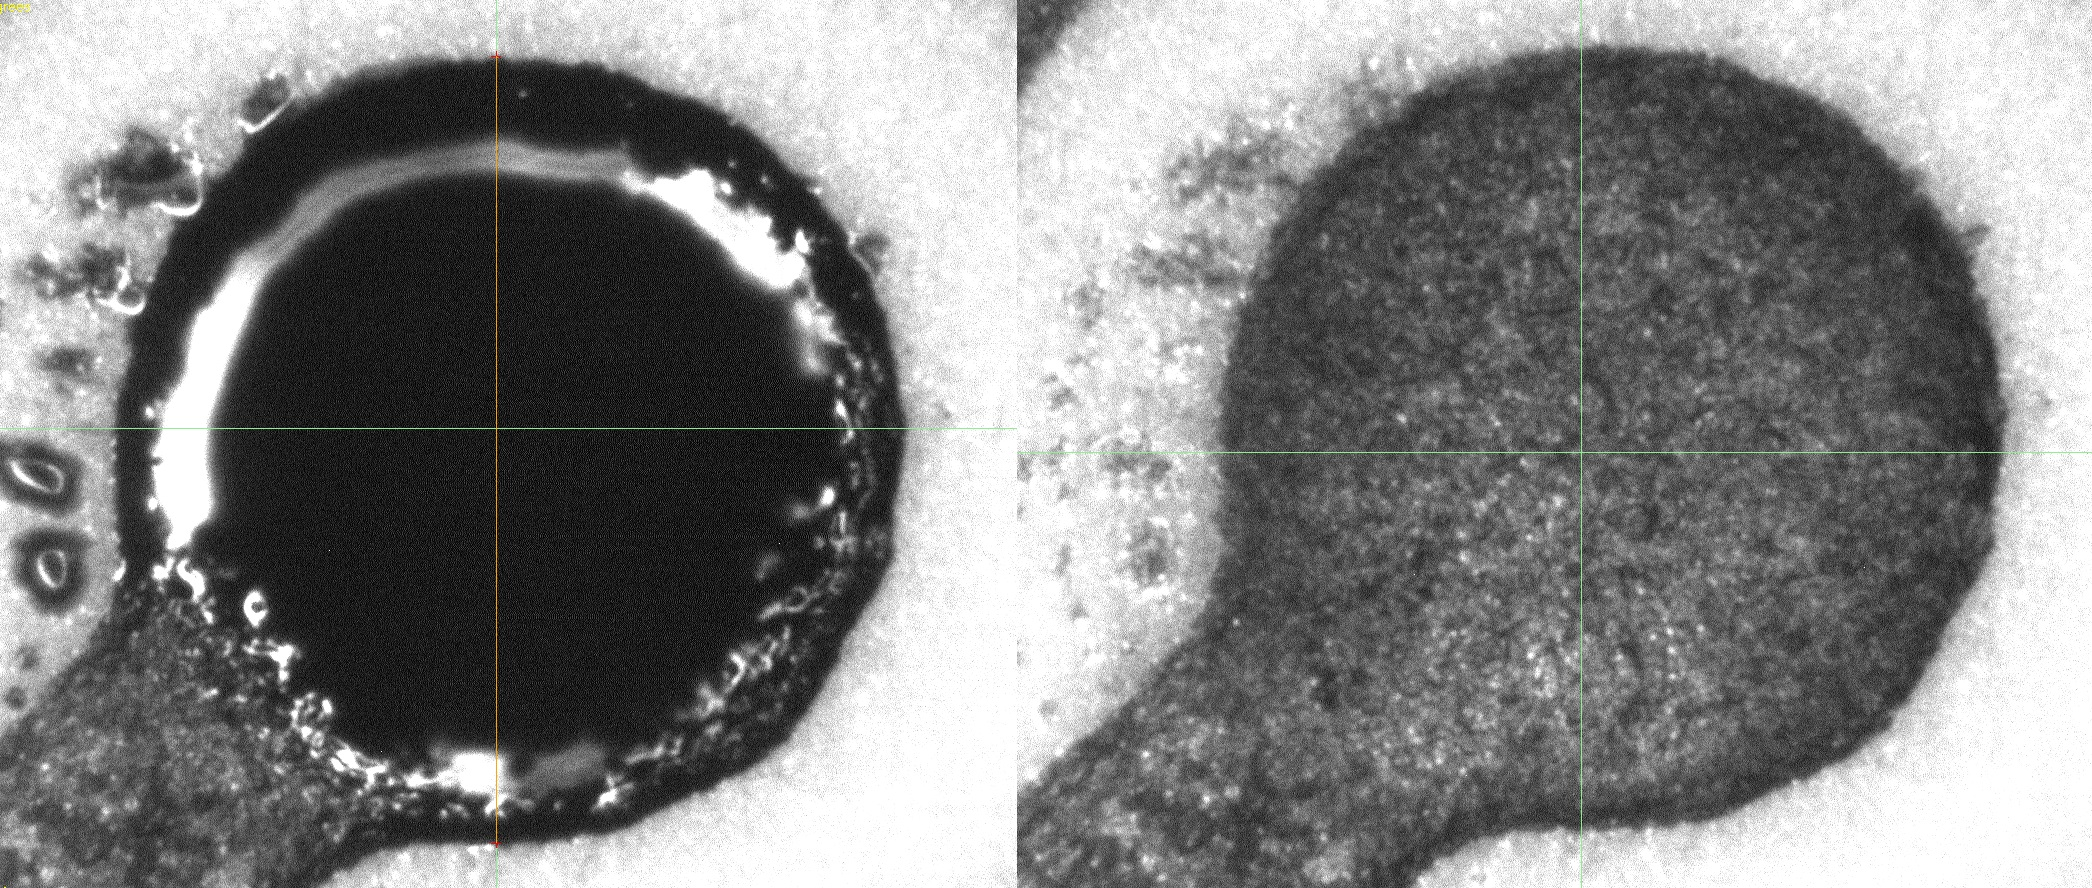
\includegraphics[width=0.5\textwidth]{Figuras/Figura_Primera_impresion_circulo}
  \caption{Primera impresión sobre electrodo de trabajo (WE1).}
  \label{fig:Figura_Primera_impresion_circulo}
\end{figure}

Se concluye que el tiempo promedio necesario para el secado de la tinta es de 10 minutos. La tinta no estará completamente seca y anclada hasta se realice el curado de la misma. Para el procedimiento de curado de la tinta de oro sobre sustrato \textit{Valox} se utiliza un \textit{Hot Plate} a 80ºC por 80 minutos (Figura ~\ref{fig:Figura_Hot_Plate}). 

\begin{figure}[H]
  \centering
    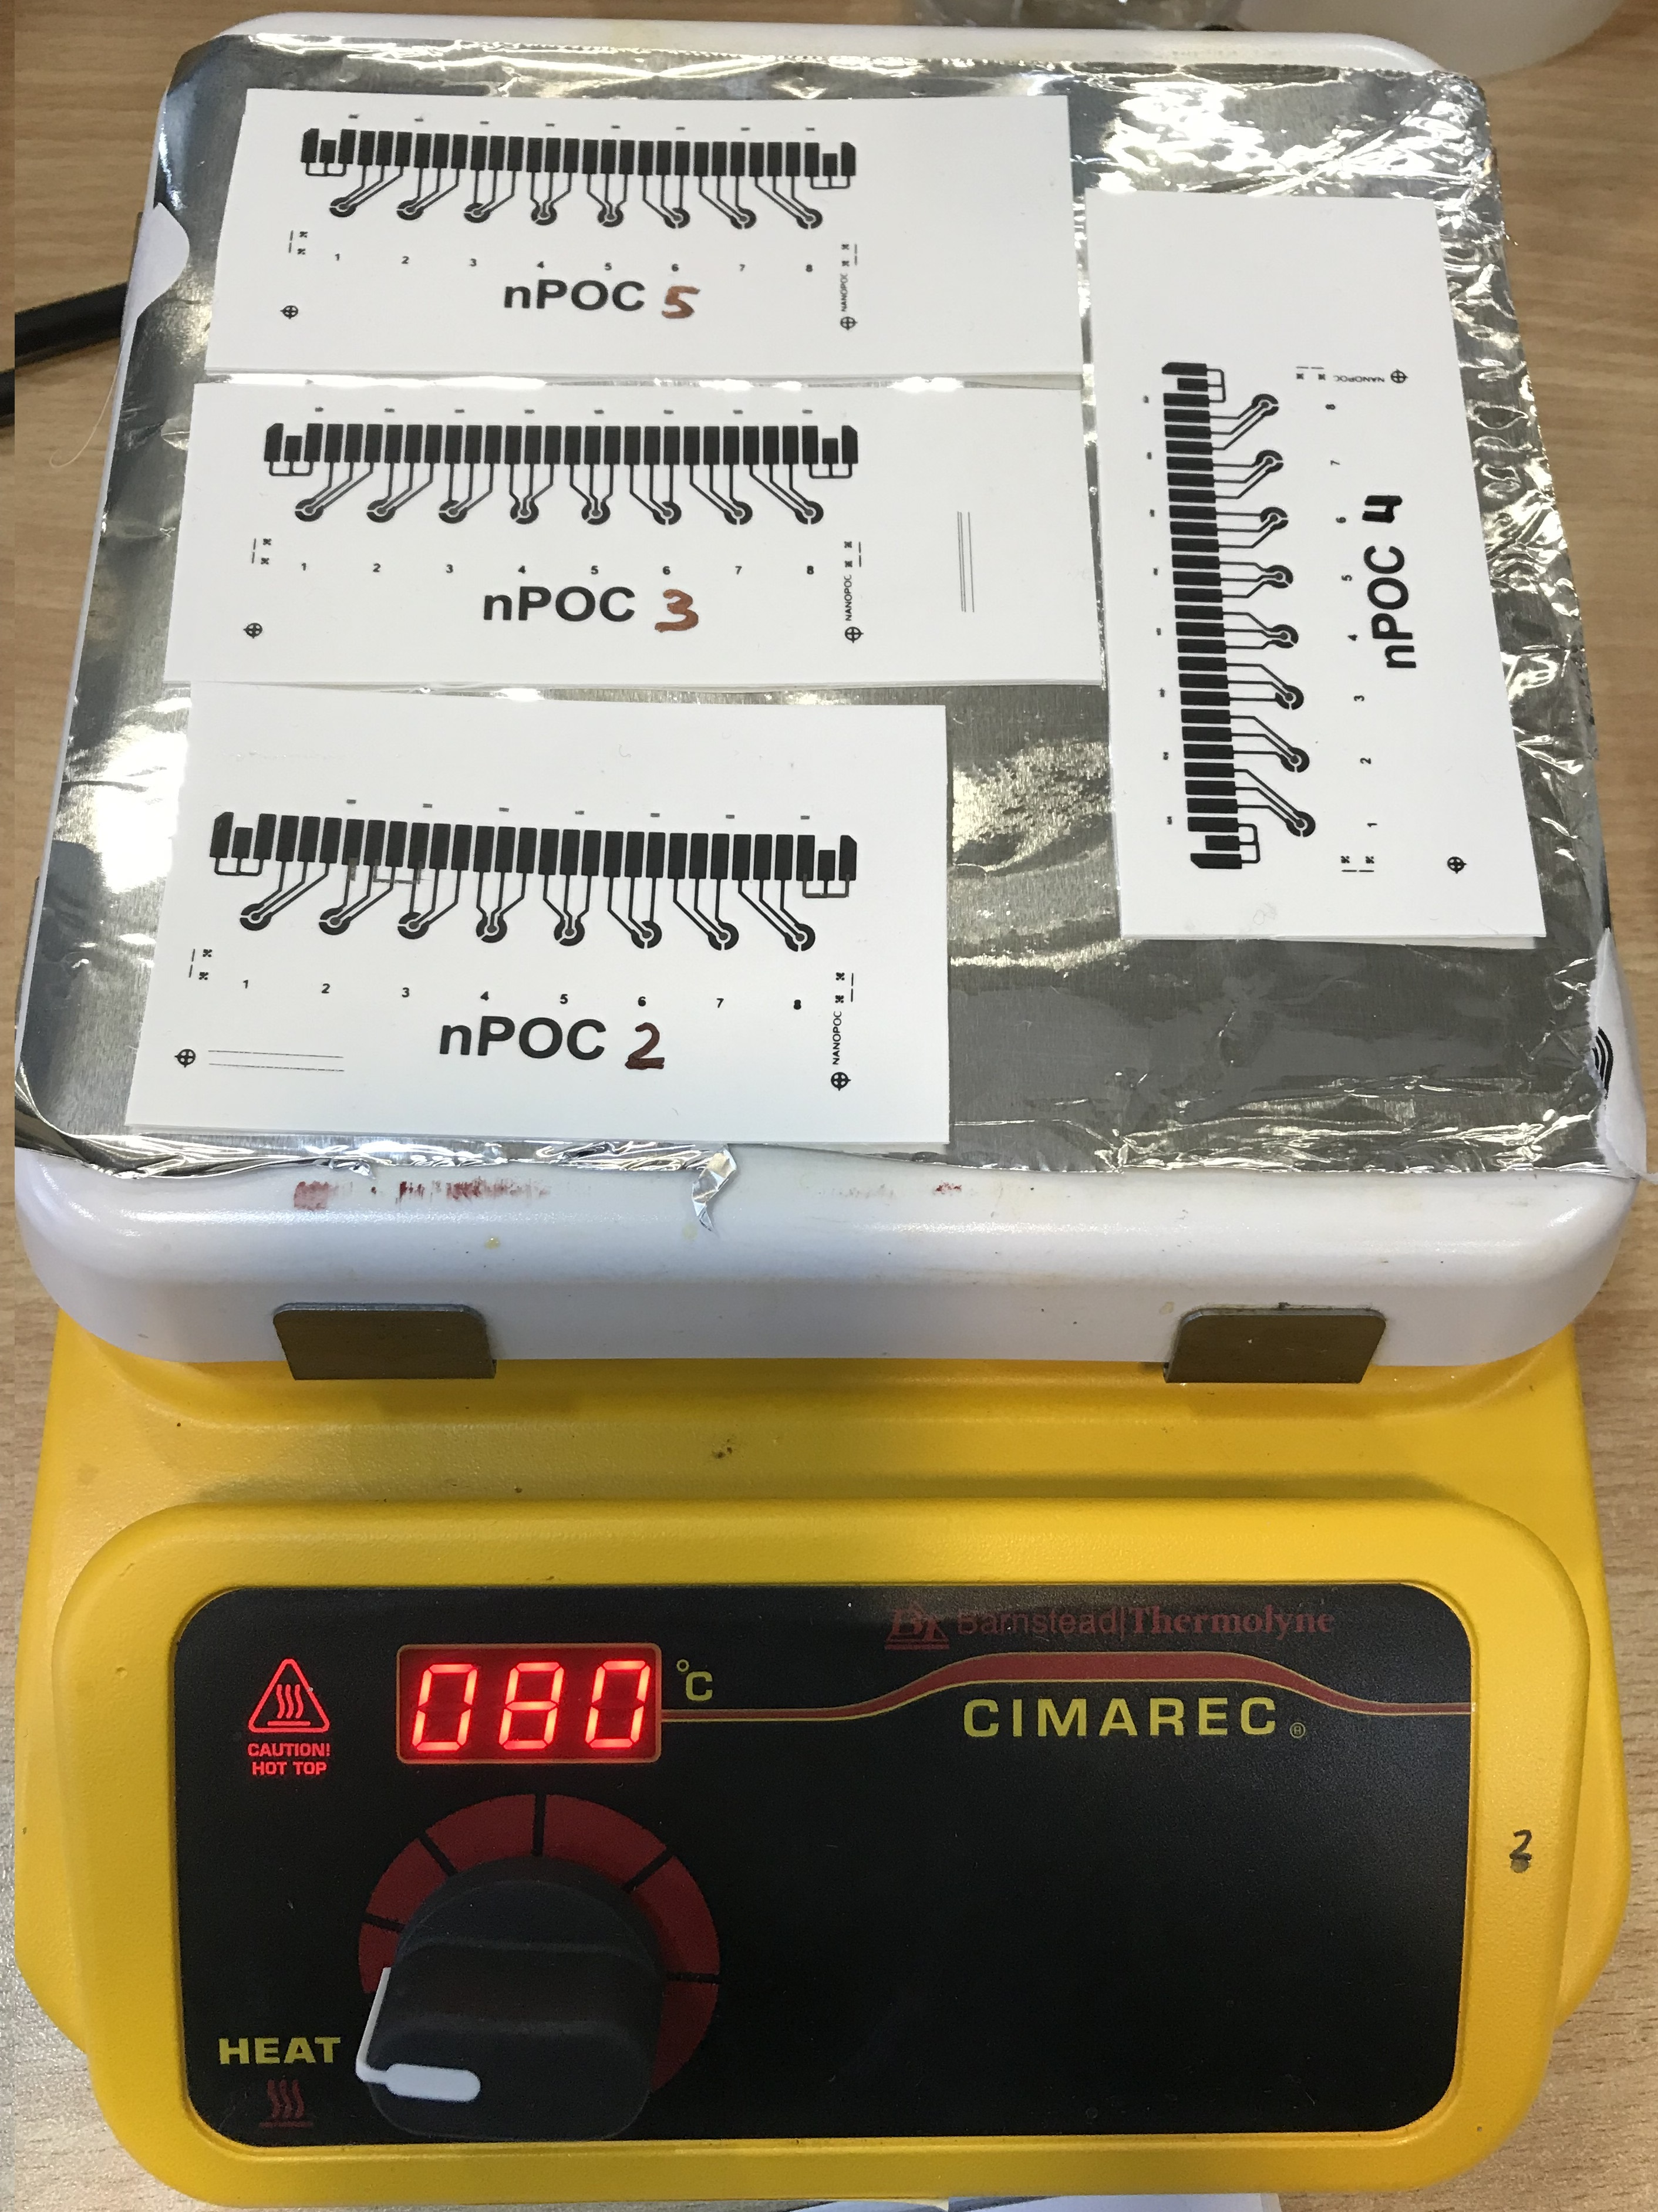
\includegraphics[width=0.4\textwidth]{Figuras/Figura_Hot_Plate}
  \caption{Curado de electrodos en \textit{Hot Plate}.}
  \label{fig:Figura_Hot_Plate}
\end{figure}

La segunda impresión se realiza con círculos de 1,1 mm de diámetro, para comparar los resultados con la impresión anterior. Se imprimen los 8 electrodos de trabajo del \textit{nPoc5}, uno a la vez. Como se puede observar (Figura ~\ref{fig:Figura_Segunda_Impresion_circulo}), la tinta que cae sobre el sustrato no se ancla correctamente generando \textit{clusters} de la misma fuera del \emph{WE}.

\begin{figure}[H]
  \centering
    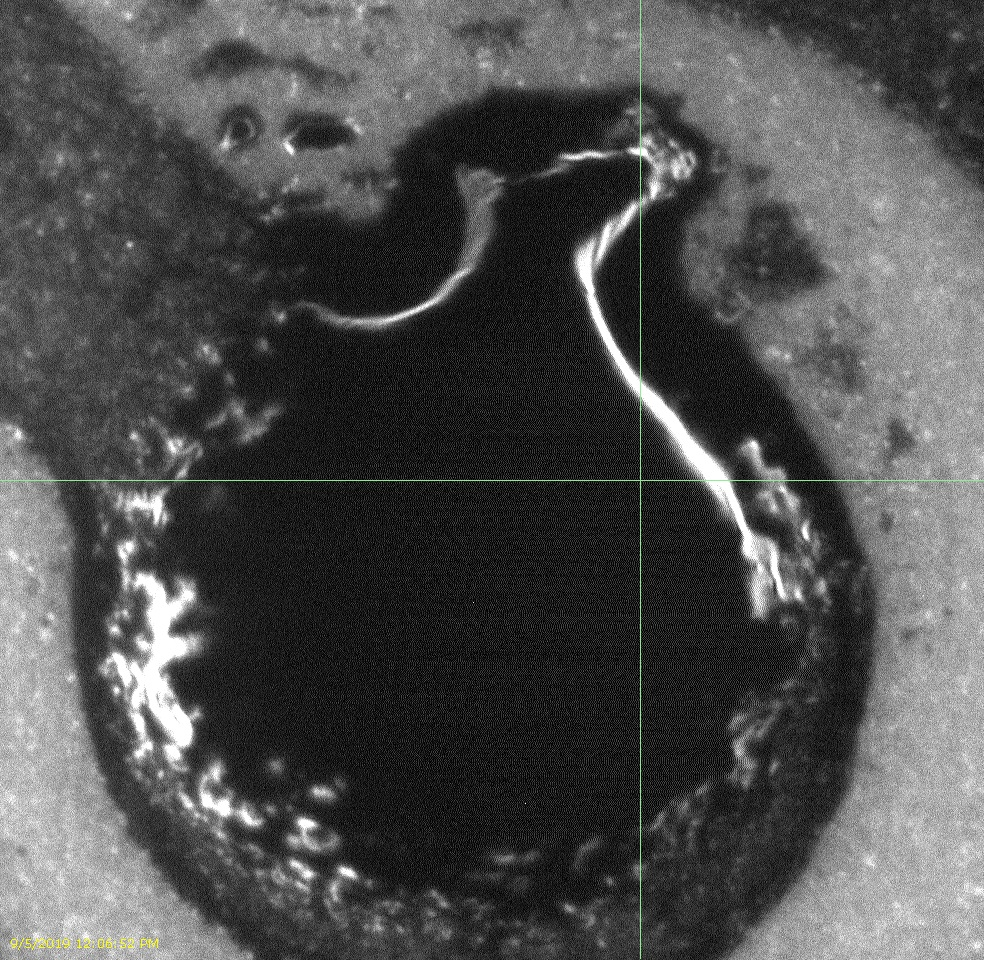
\includegraphics[width=0.45\textwidth]{Figuras/Figura_Segunda_Impresion_circulo}
  \caption{Impresión de círculo de 1,1 mm sobre \emph{WE}.}
  \label{fig:Figura_Segunda_Impresion_circulo}
\end{figure}

Para aumentar el nivel de reproducibilidad a mayor escala, se diseña un patrón de ocho círculos de 1 mm de diámetro cada uno. El punto de referencia se centra en el primer círculo y se alinea con el centro del primer \emph{WE} del sustrato \textit{nPoc3}.

Al revisar la impresión se notan pequeñas desviaciones en la deposición de la tinta de oro, esto puede deberse a las variaciones que se obtienen por la impresión serigráfica del patrón de tinta de carbono. Sin embargo, no se detectan derrames de tinta considerables sobre el sustrato \textit{Valox} (Figura ~\ref{fig:Figura_impresion_8juntos}).

\begin{figure}[H]
  \centering
    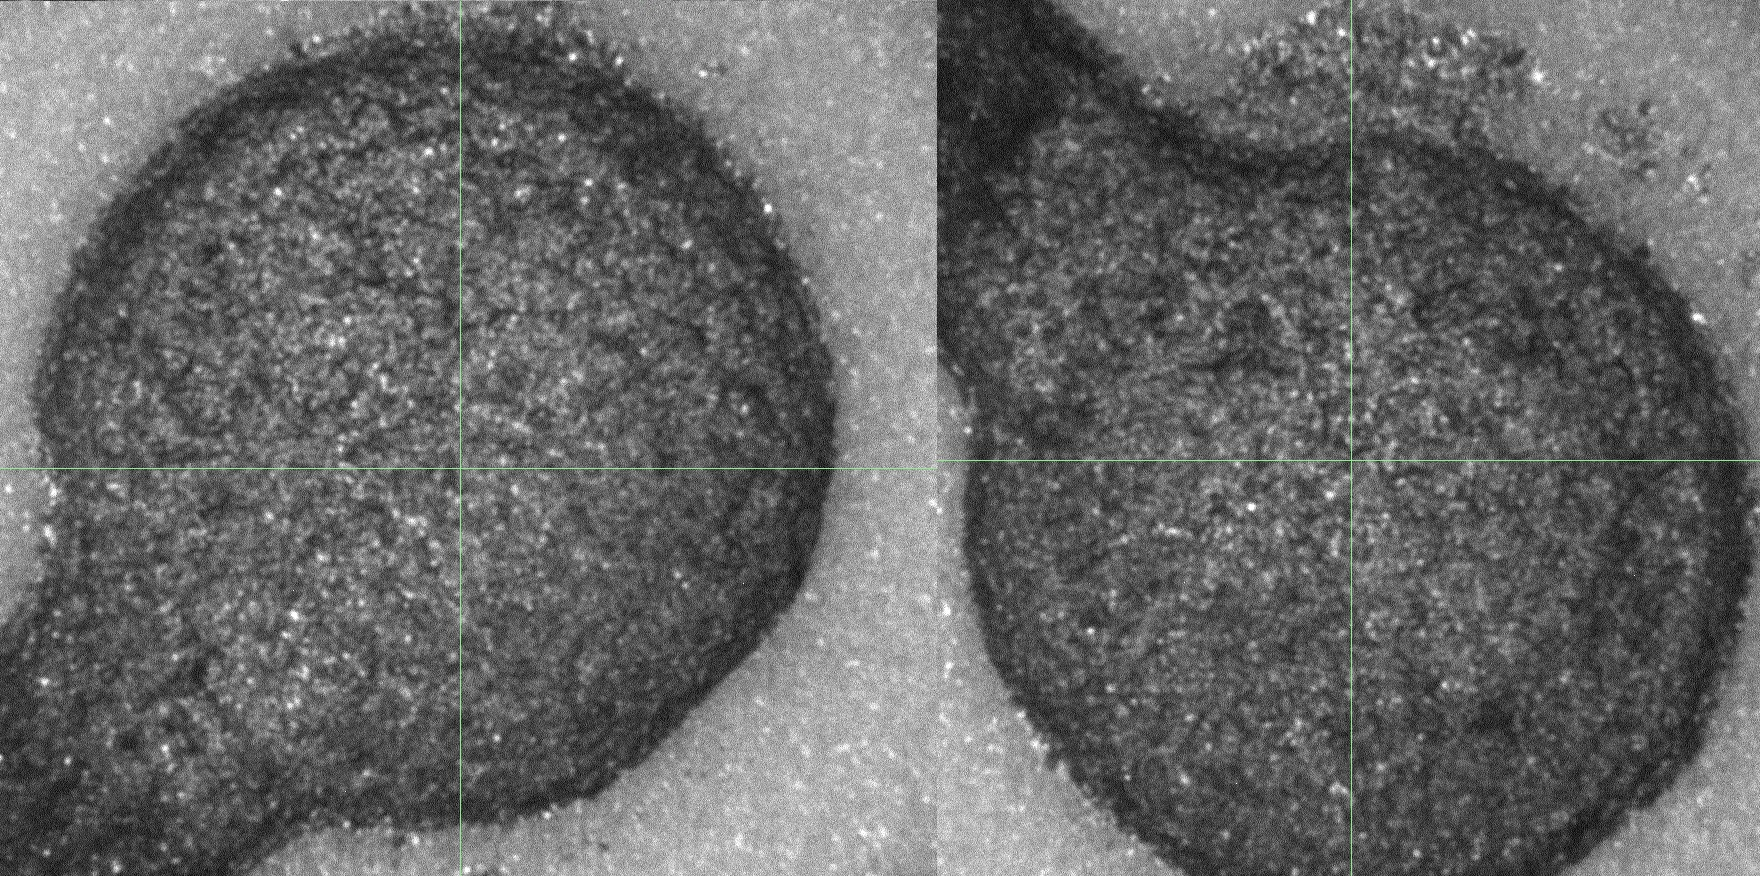
\includegraphics[width=0.6\textwidth]{Figuras/Figura_impresion_8juntos}
  \caption{Comparación de impresión entre \emph{WE} 3 y 5.}
  \label{fig:Figura_impresion_8juntos}
\end{figure}

A continuación, se cura el biosensor sobre un \textit{Hot Plate} a 80ºC por 80 minutos. Se observa que la tinta toma un color más claro, semejante al color del oro puro (Figura ~\ref{fig:Figura_impresion_curado}).

\begin{figure}[H]
  \centering
    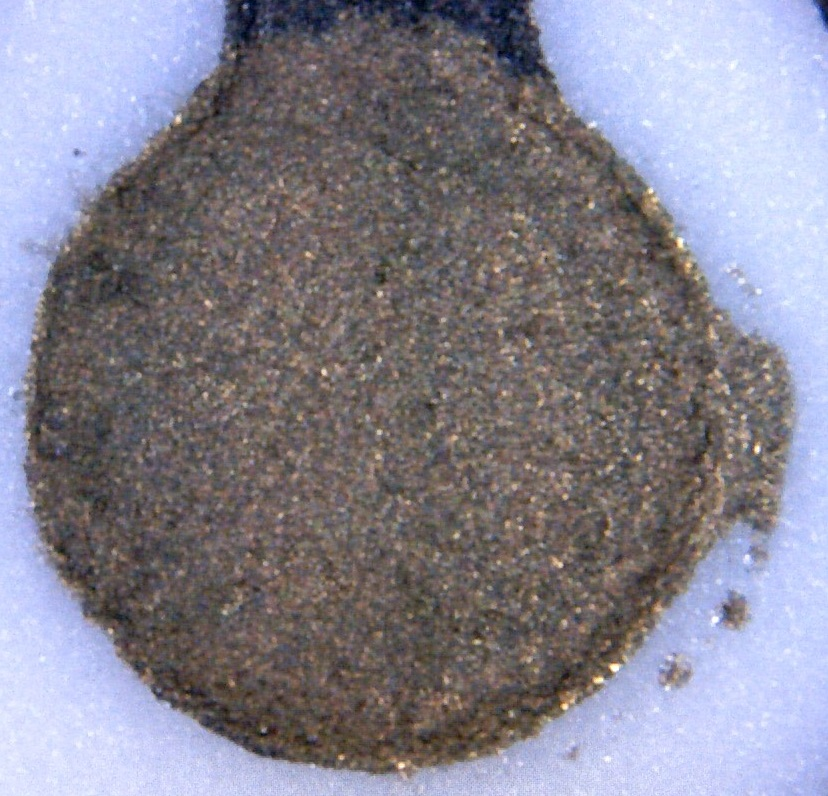
\includegraphics[width=0.45\textwidth]{Figuras/Figura_impresion_curado}
  \caption{Imágen con microscopio USB 1000X de \emph{WE} curado en \textit{Hot Plate}.}
  \label{fig:Figura_impresion_curado}
\end{figure}

Para la caracterización eléctrica se diseñó un patrón con la forma de conexión entre dos contactos de prueba del biosensor (Figura ~\ref{fig:Figura_contactos_prueba}).

\begin{figure}[H]
  \centering
    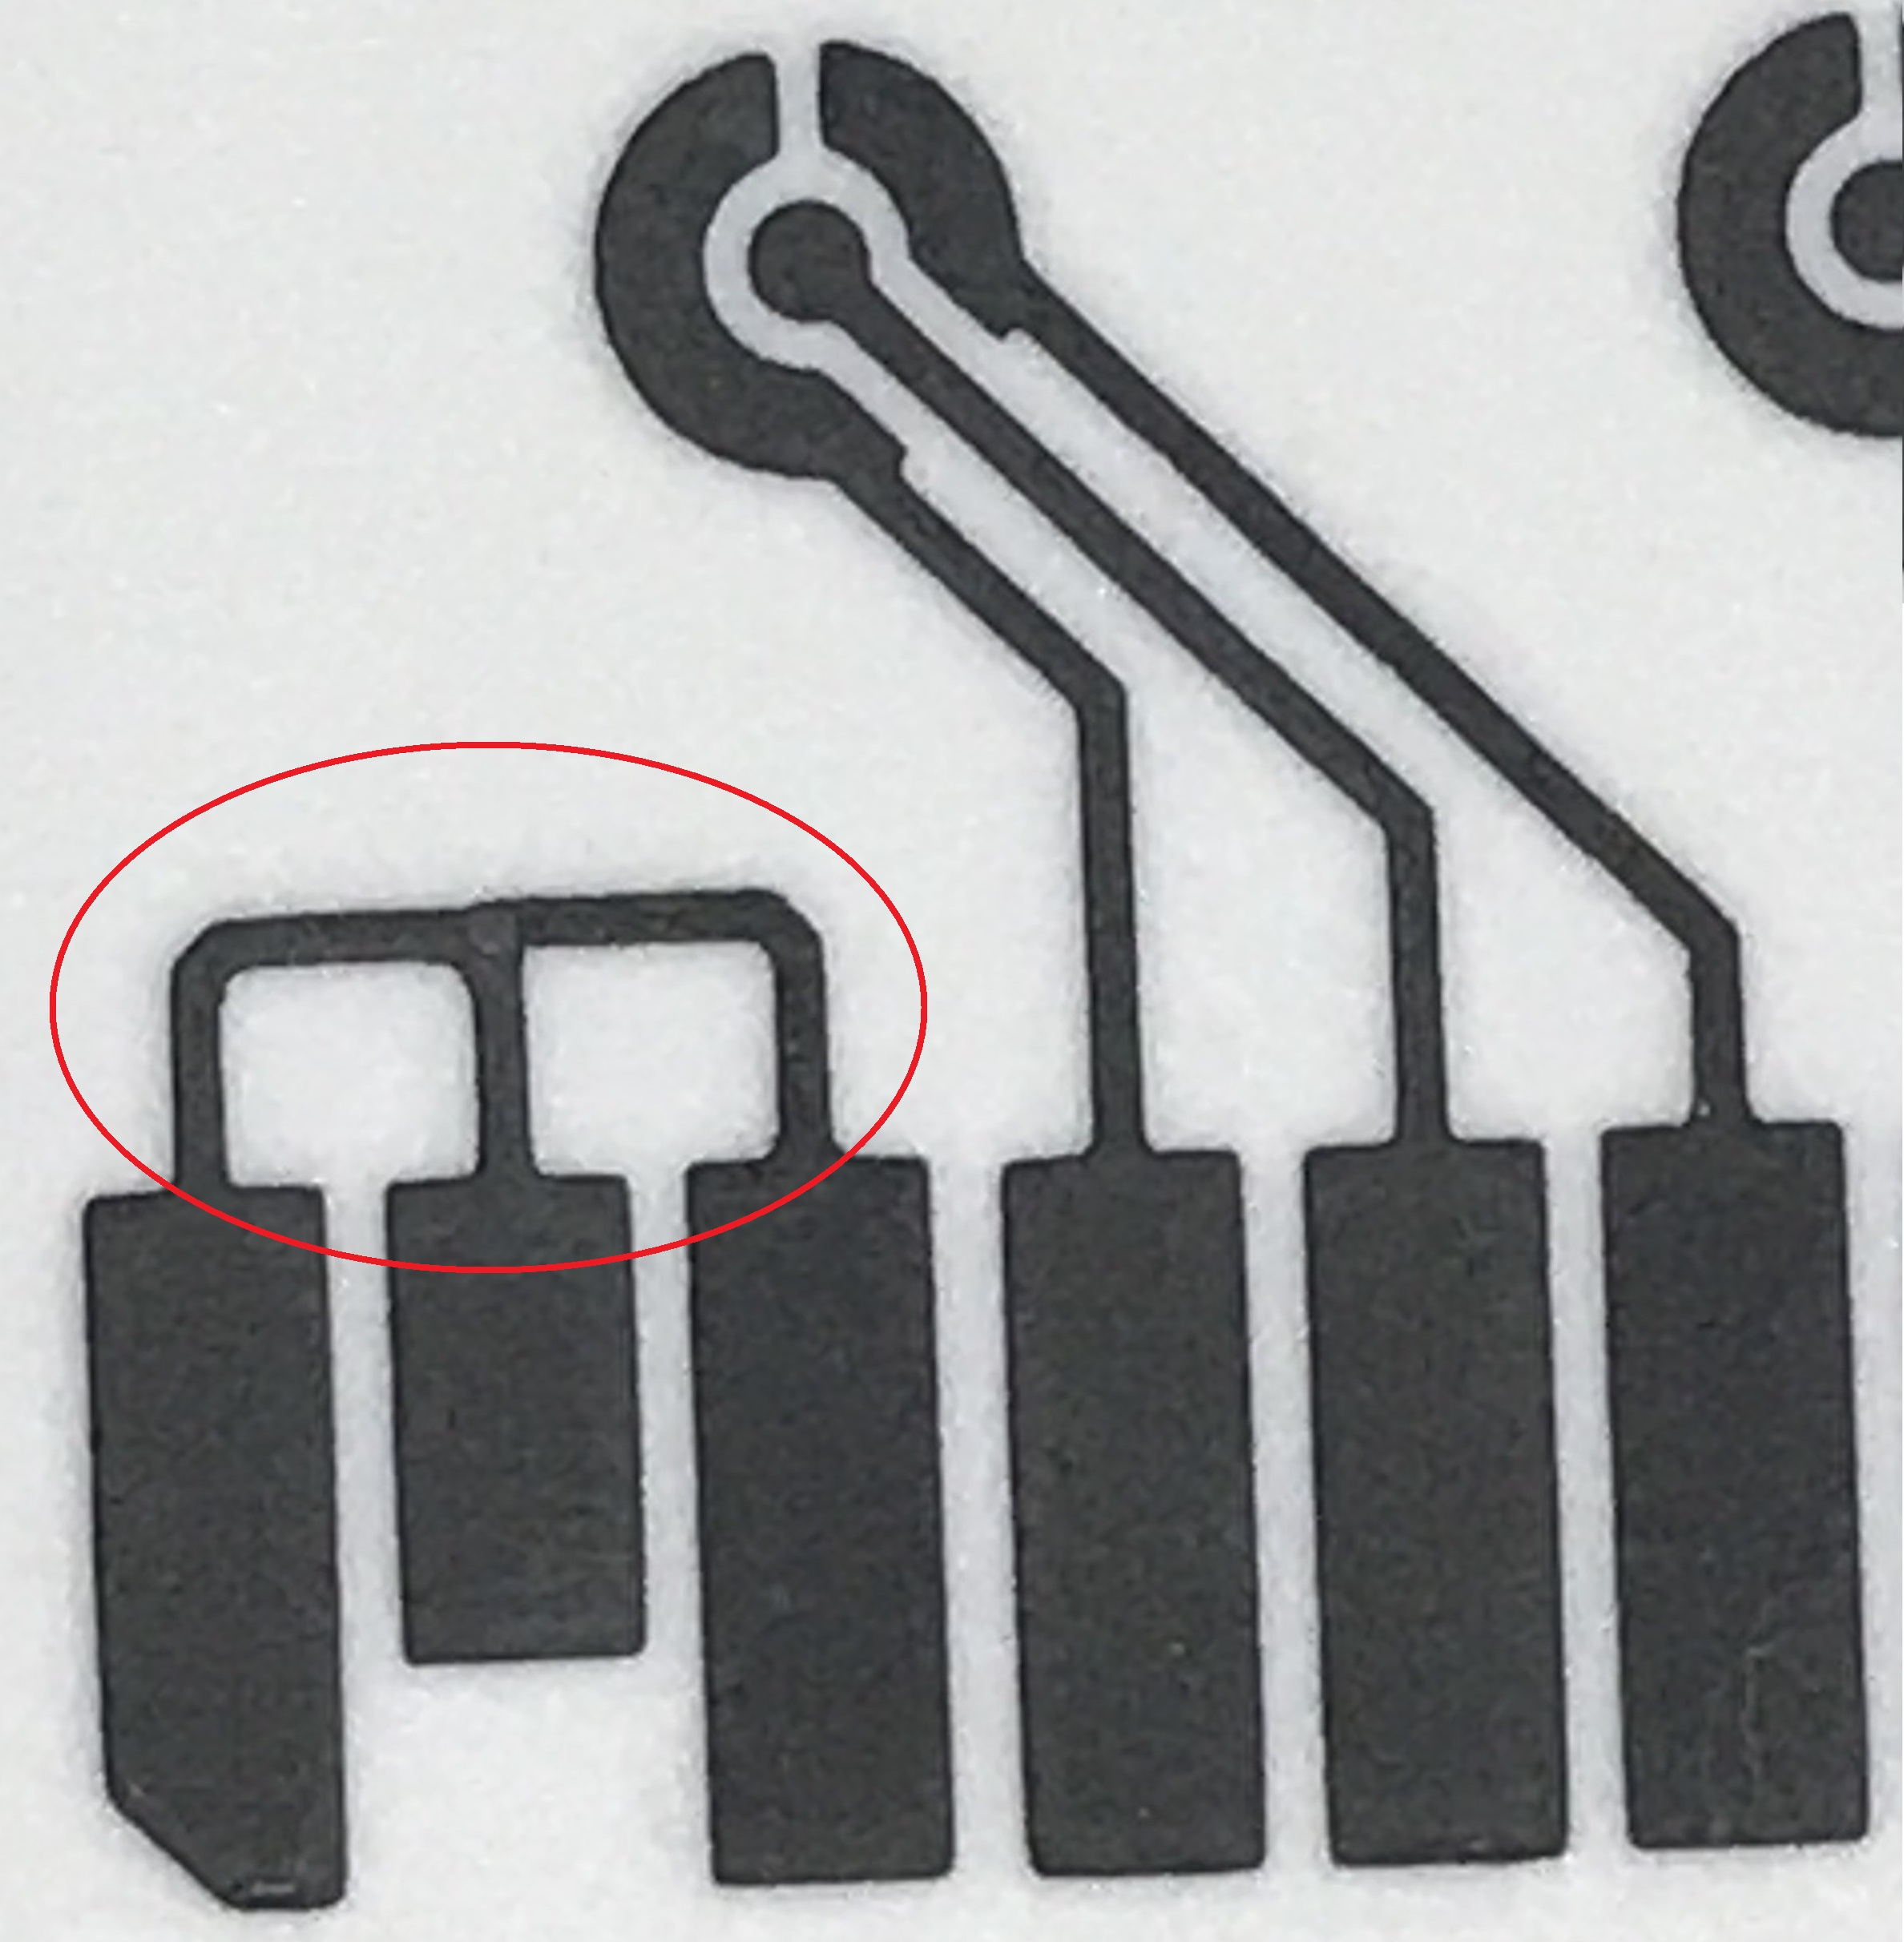
\includegraphics[width=0.45\textwidth]{Figuras/Figura_contactos_prueba}
  \caption{Contactos de prueba en biosensor.}
  \label{fig:Figura_contactos_prueba}
\end{figure}

El diseño tiene 2,5 mm de alto y 5,5 mm de largo, el ancho de las vías es de 0,4 mm. Para esta impresión no se utilizó punto de referencia sino que se agregó el punto de origen de impresión alineado con el comienzo de las vías de carbono. Se añadió 1 mm sobre los contactos para tener una mejor relación carbono-nanopartículas de oro. Dado el buen anclaje de la tinta de nanopartículas de oro sobre el carbono se obtuvo correctamente el diseño buscado, casi sin derrames (Figura ~\ref{fig:Figura_contactos_prueba_con_Oro}). Se imprimieron dos capas del diseño, ambas curadas en \textit{Hot Plate} a 80ºC por 80 minutos.

\begin{figure}[H]
  \centering
    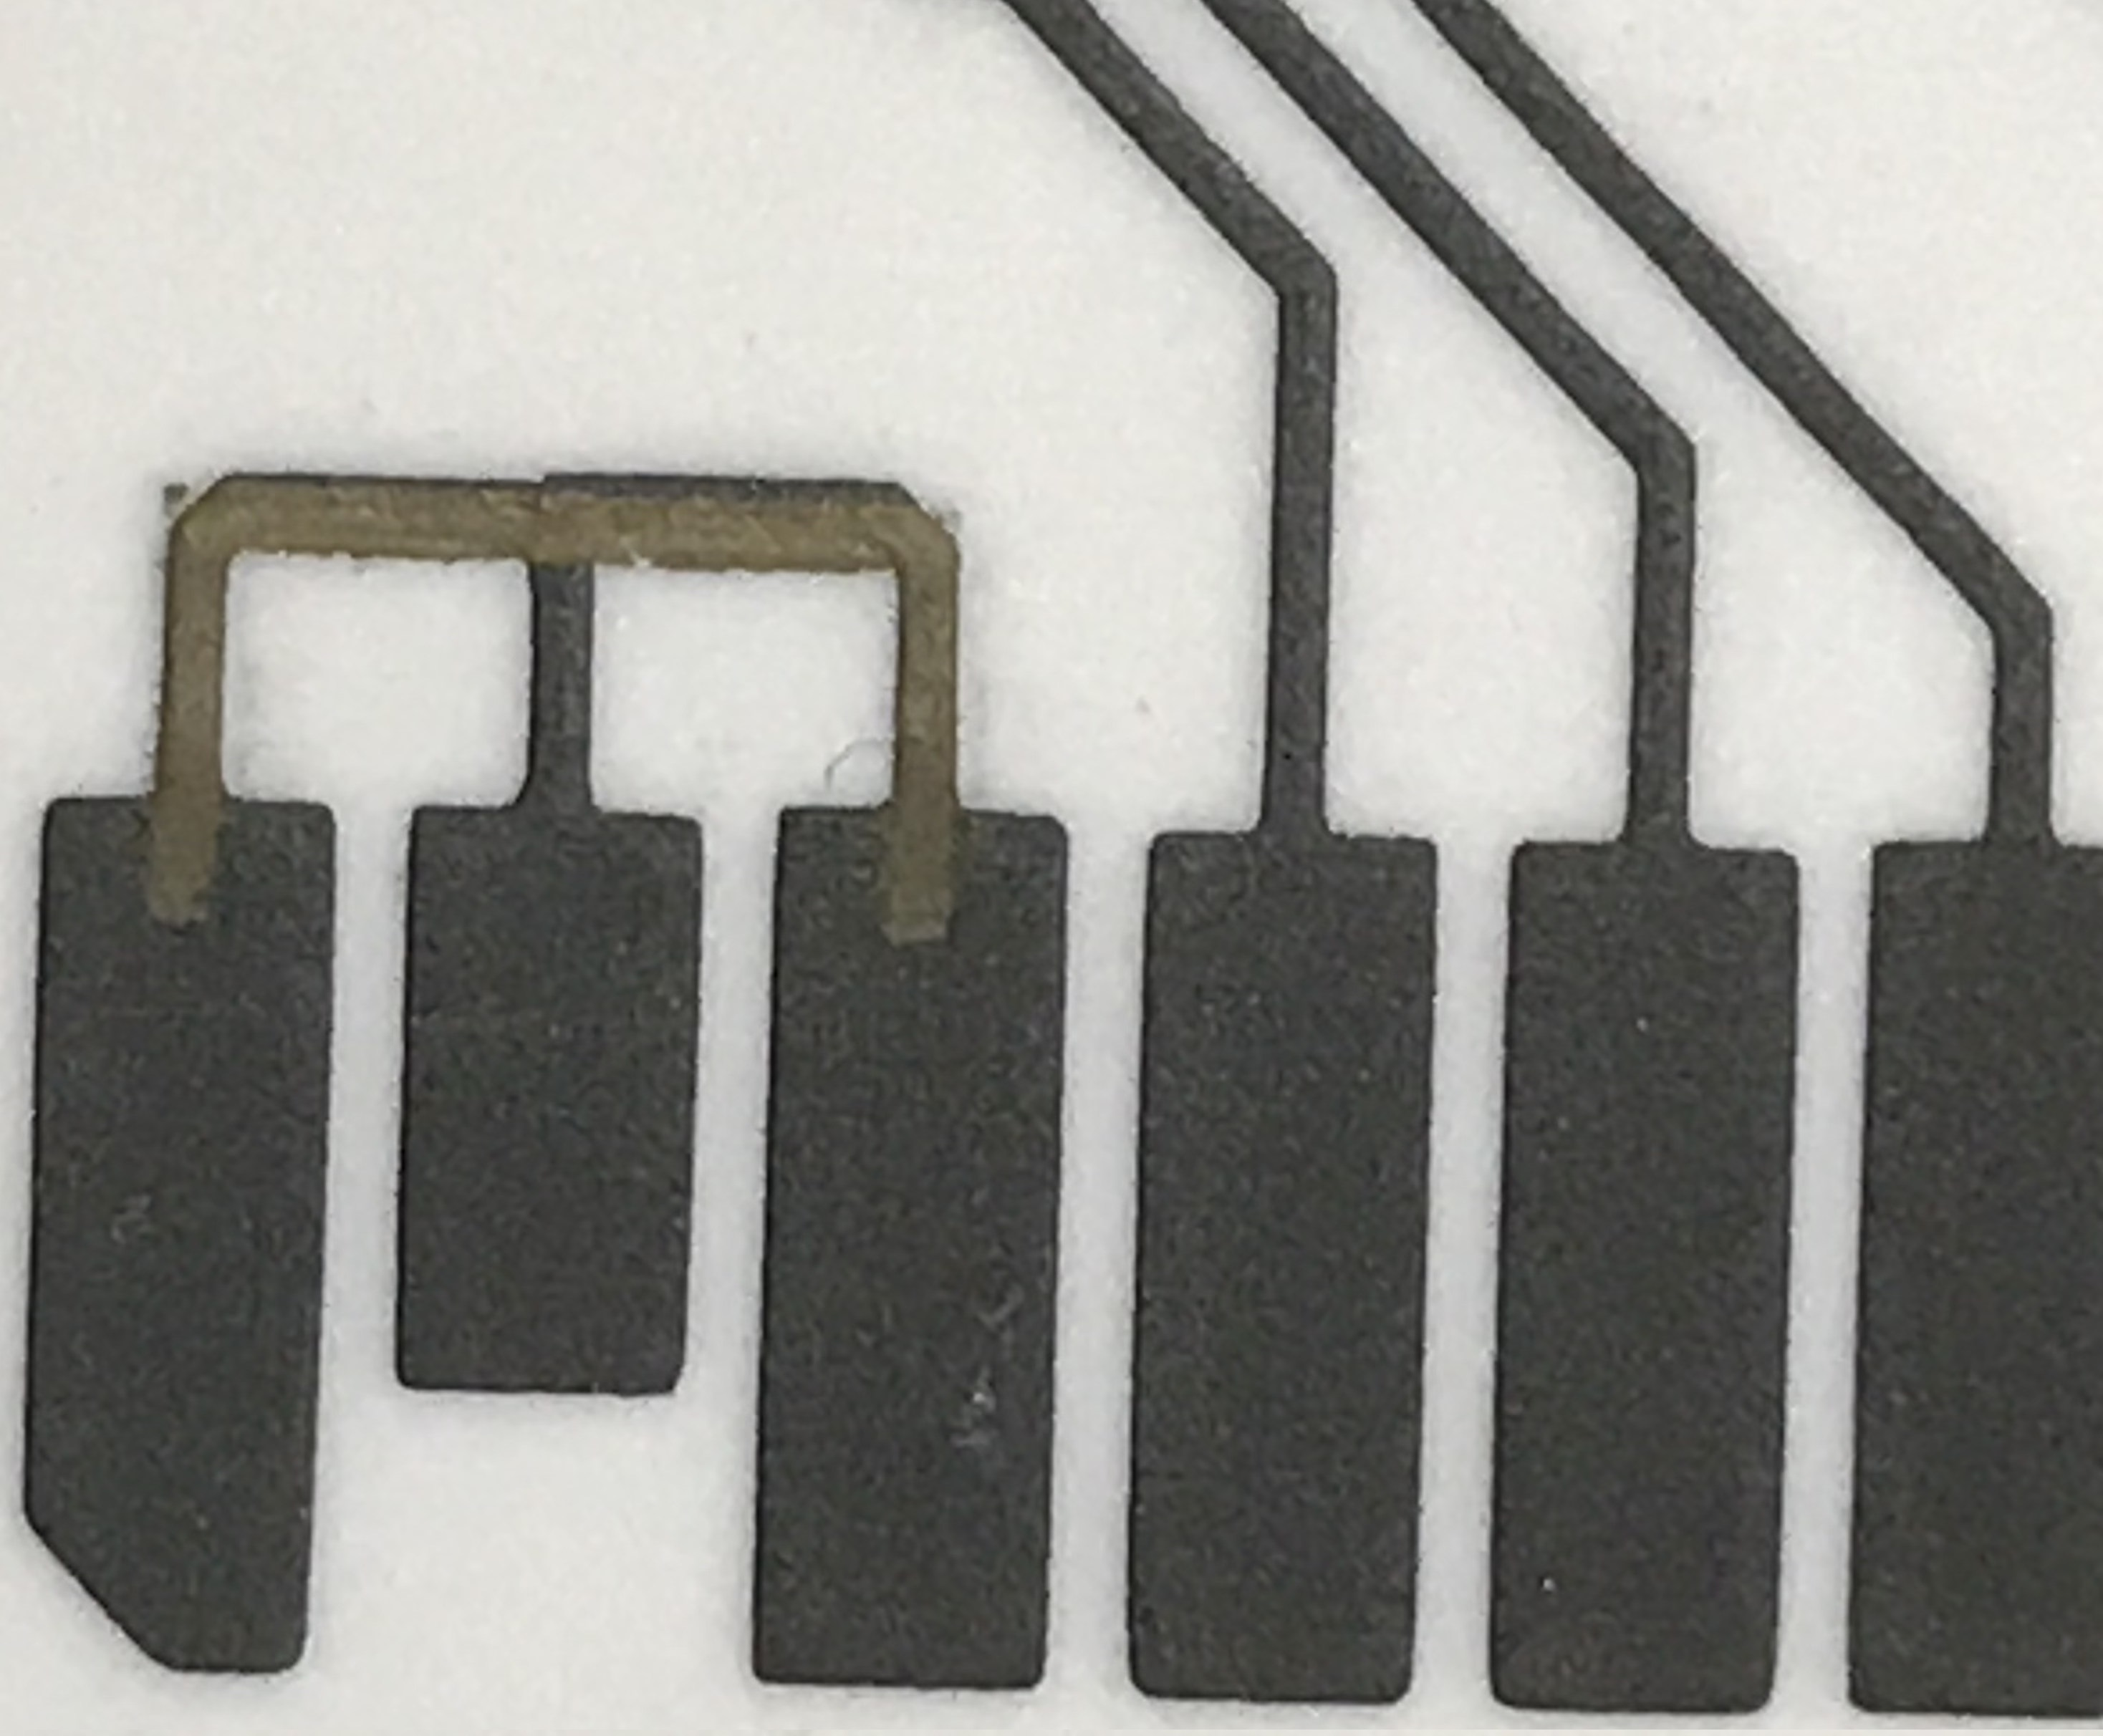
\includegraphics[width=0.45\textwidth]{Figuras/Figura_contactos_prueba_con_Oro}
  \caption{Contactos de prueba con impresión de tinta con nanopartículas de oro.}
  \label{fig:Figura_contactos_prueba_con_Oro}
\end{figure}

Para tener mayor cantidad de pruebas en la caracterización electroquímica se realizaron impresiones con tinta de nanopartículas de oro sobre el sustrato \textit{Valox}, sin tinta de carbono (Figura ~\ref{fig:Figura_impresion_sustrato_valox_tinta_Oro}), sobre un sustrato PET (Tereftalato de polietileno) y una hoja de pulpa de celulosa (hoja de cuaderno convencional).

\begin{figure}[H]
  \centering
    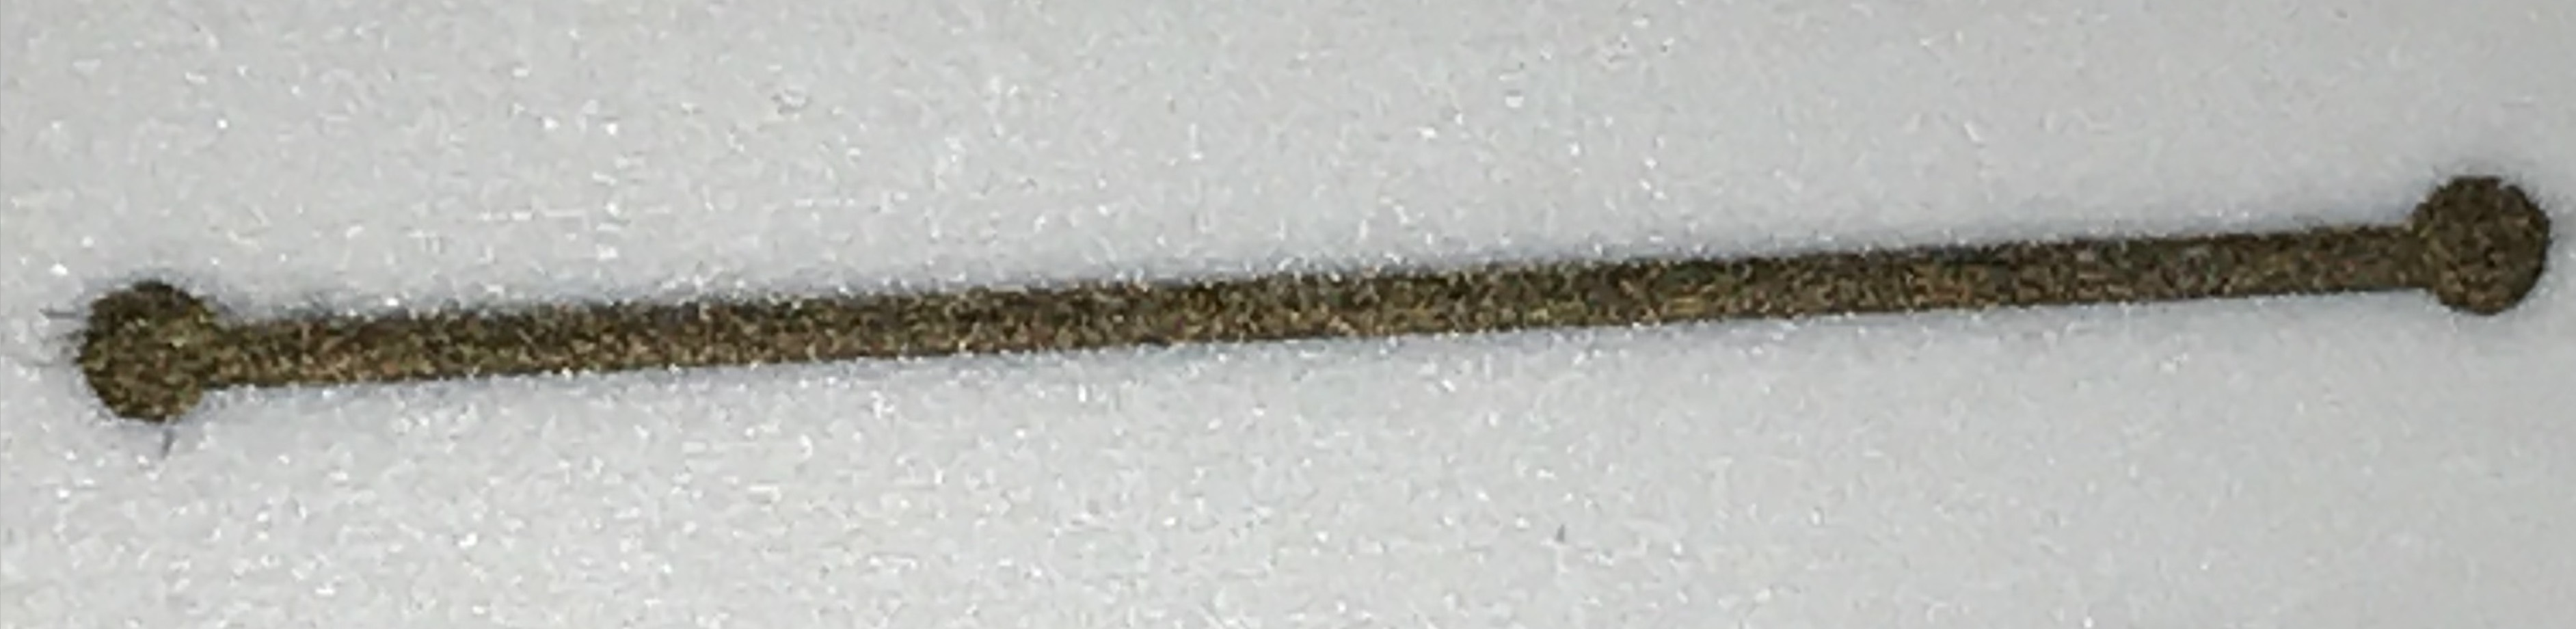
\includegraphics[width=0.5\textwidth]{Figuras/Figura_impresion_sustrato_valox_tinta_Oro}
  \caption{Impresión sobre sustrato Valox.}
  \label{fig:Figura_impresion_sustrato_valox_tinta_Oro}
\end{figure}

Sobre el sustrato \textit{Valox} y la hoja de pulpa de celulosa se imprimieron dos círculos de 1 mm de diámetro separados 16 mm que luego fueron unidos por una línea de 17 mm de largo y 0,4 mm de ancho, de esta forma la tinta se imprimió desde la mitad de un círculo hasta la mitad del otro, asegurando la continuidad del material. Se imprimieron dos capas idénticas, para el sustrato \textit{Valox} se realizó un curado entre cada impresión en \textit{Hot Plate} a 80ºC por 80 minutos.

Para el sustrato PET se realizó un diseño diferente (Figura ~\ref{fig:Figura_impresion_sobre_PET}) debido a que no se tenía referencia de cómo se anclaría la tinta sobre la base. Se realizó un arreglo de seis dibujos en dos columnas, compuestos por dos cuadrados de 1 mm de lado separados 16 mm y una barra de 17 mm de largo y 0,4 mm de ancho. La separación entre columnas es de 65 mm y 20 mm entre filas. La separación en columnas se debe a que la mitad del sustrato se limpió superficialmente con alcohol etílico, de esta forma, se buscó obervar las diferencias entre el sustrato tratado y sin tratar. Se imprimieron dos capas idénticas con sus respectivos curados en \textit{Hot Plate} a 80ºC por 80 minutos.

\begin{figure}[H]
  \centering
    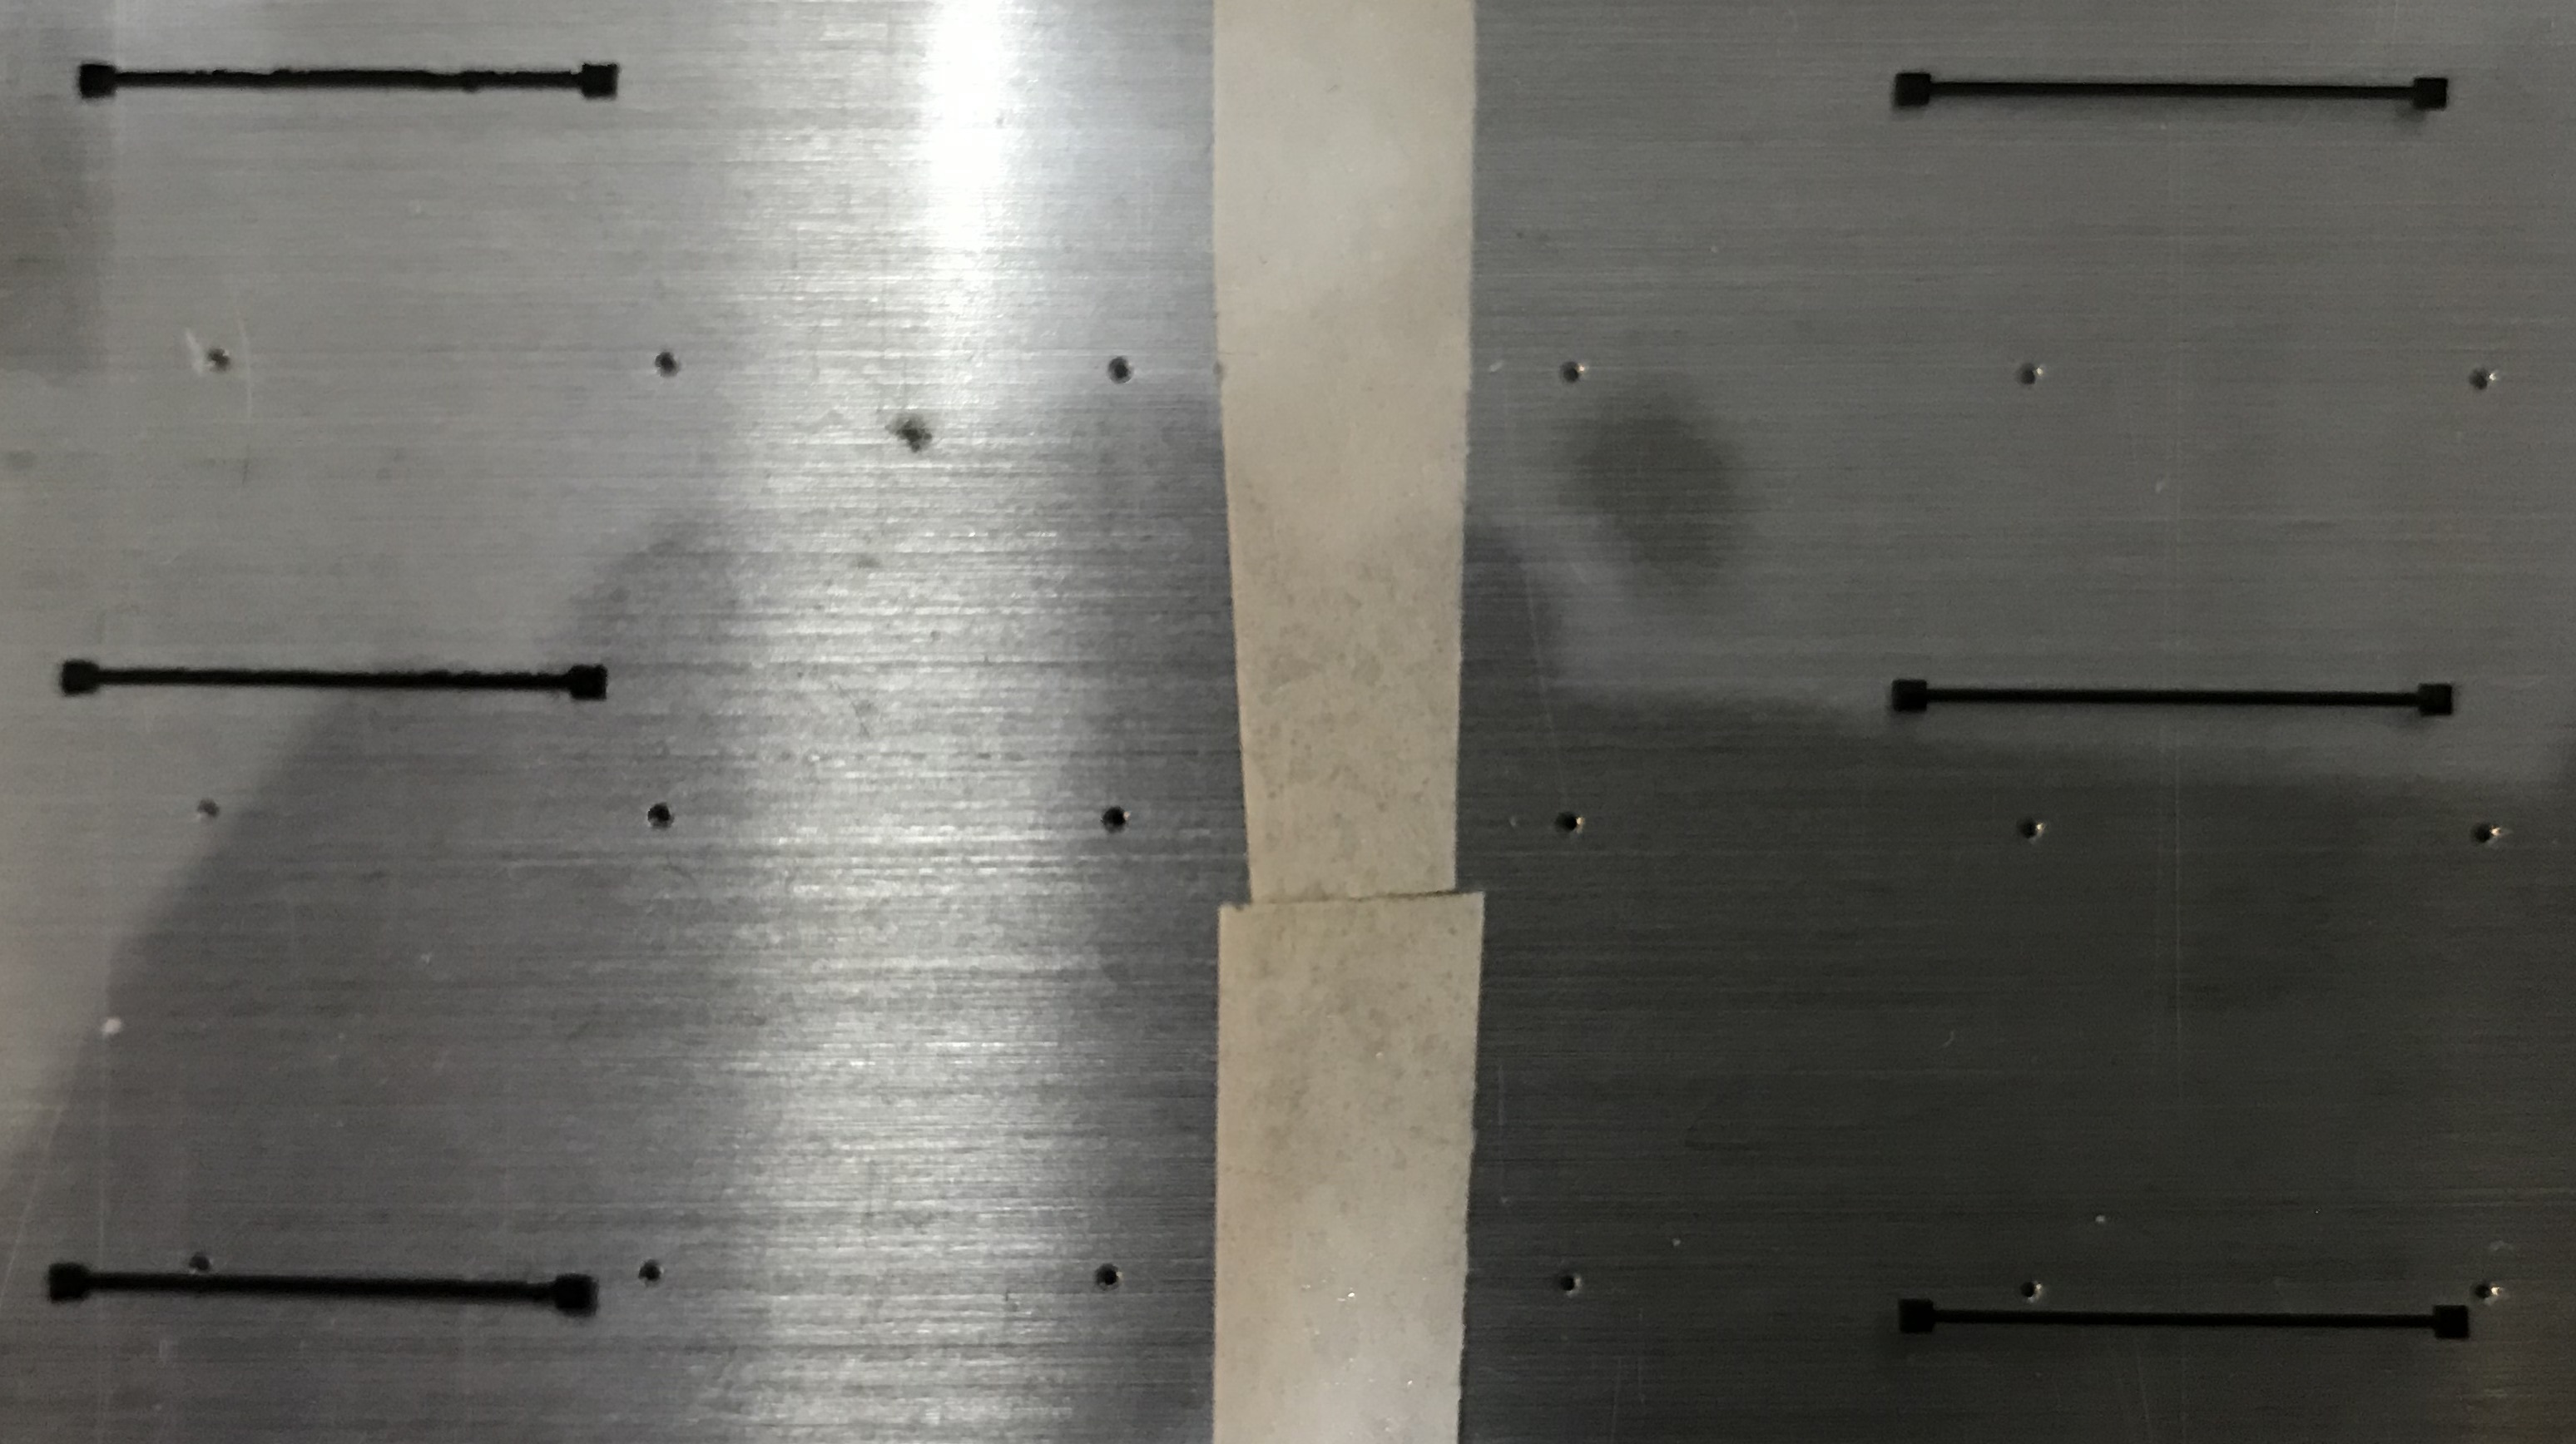
\includegraphics[width=0.5\textwidth]{Figuras/Figura_impresion_sobre_PET}
  \caption{Diseño impreso sobre sustrato PET.}
  \label{fig:Figura_impresion_sobre_PET}
\end{figure}

\section{Caracterizaciones}
\subsection{Caracterización eléctrica}
La caracterización eléctrica consta de la medición de resistencia a 4 puntas, explicada anteriormente en el Capítulo 2, \hyperref[subsec:carac_elec]{apartado 2.3.1}. Las mediciones de resistencia se hicieron sobre tinta de carbono, tinta de carbono más una capa y más dos capas de tinta de nanopartículas de oro curado.

Se debe tener en cuenta que los resultados obtenidos de esta medición se compone de un paralelo eléctrico entre la resistencia de la tinta de carbono y la resistencia de la tinta de nanopartículas de oro. Se obtuvo un descenso considerable de la resistencia (en comparación de un paralelo de dos resistencias de carbono) en concordancia con la teoría propuesta, dado que la resistividad del oro (2.44·10\textsuperscript{-8} Ohm·m) es mucho menor a la del carbono (3.5·10\textsuperscript{-5} Ohm·m) \cite{Resistividad}.

\subsection{Caracterización dimensional}
Para la caracterización dimensional se utilizó la cámara fiducial de la impresora \textit{Dimatix}, obteniendo las dimensiones de los \emph{WE} y las separaciones entre este, el \emph{CE} y el \emph{RE} (Figura ~\ref{fig:Figura_medicion_WE}).

\begin{figure}[H]
  \centering
    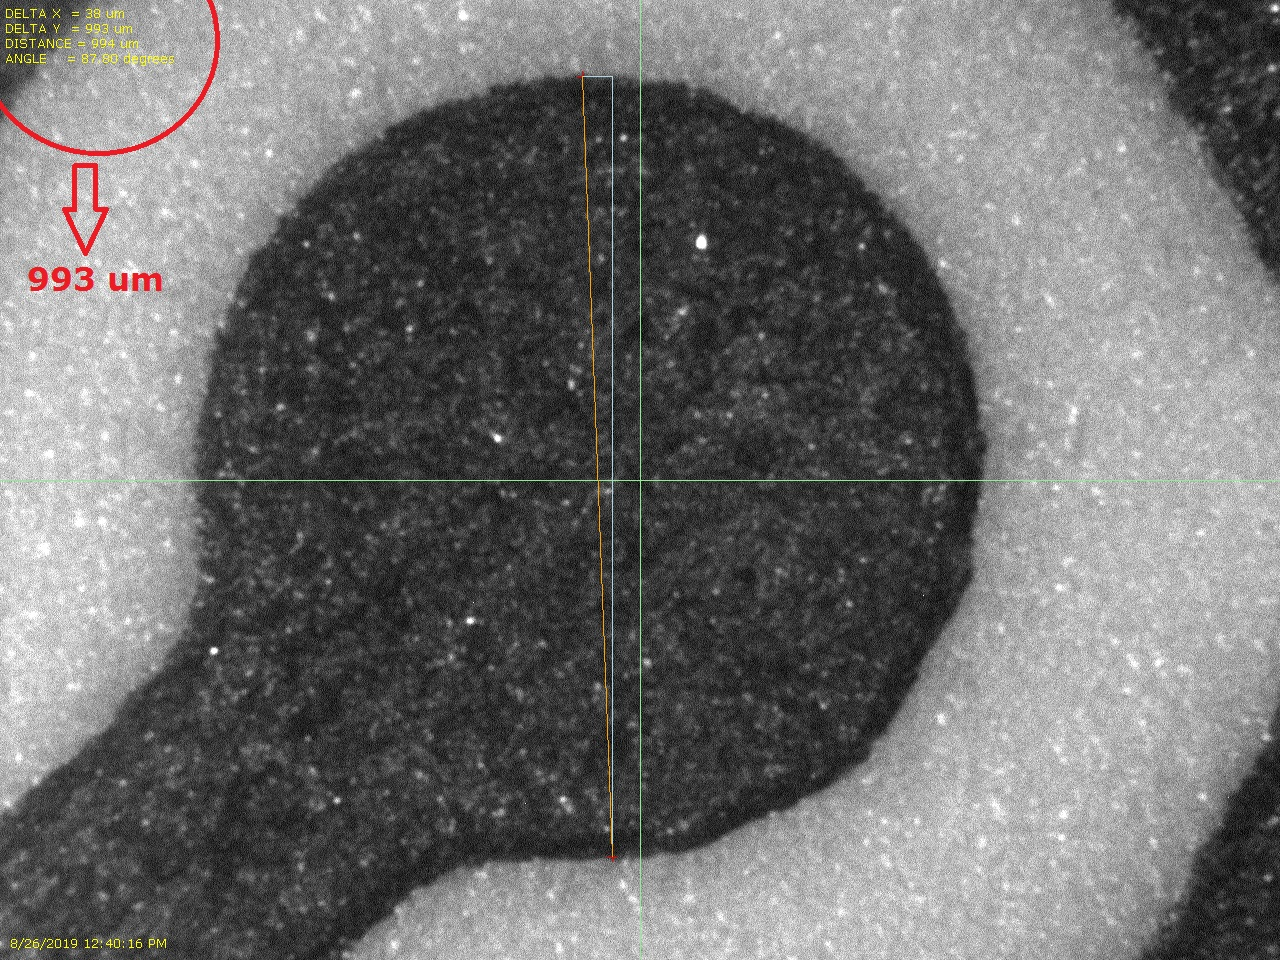
\includegraphics[width=0.5\textwidth]{Figuras/Figura_medicion_WE}
  \caption{Medición del diámetro del \emph{WE}.}
  \label{fig:Figura_medicion_WE}
\end{figure}

La rugosidad y los espesores de la película de carbono y de la película obtenida con la tinta de nanopartículas de oro se obtuvieron mediante un perfilómetro de contacto marca \textit{Bruker} modelo \textit{Dektak XT} con una punta \textit{Stylus} de 12,5  $\mu$m (Figura ~\ref{fig:Figura_Perfilometro}). La fuerza aplicada por la punta fue en ambos casos de 3 mgf.

\begin{figure}[H]
  \centering
    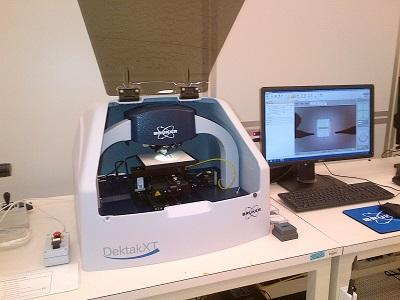
\includegraphics[width=0.5\textwidth]{Figuras/Figura_Perfilometro}
  \caption{Perfilómetro Dektak XT Advanced.}
  \label{fig:Figura_Perfilometro}
\end{figure}

Para dicha caracterización se determinó un recorrido de 2000 $\mu$m sobre el electrodo de trabajo durante 15 segundos y luego se seleccionó el área de interés para medir la rugosidad. Se tomaron tres valores sobre toda la muestra:

$\bullet$ El valor promedio de rugosidad máxima (Rz)

$\bullet$ El pico de rugosidad más alto (Rt)

$\bullet$ El valor promedio de rugosidad (Ra).
\\

Para la caracterización del espesor del \emph{WE} se fijó un recorrido de 1000 $\mu$m durante 15 segundos. El largo del recorrido se determinó en ese valor para poder obtener los escalones de subida/bajada y con esto poder obtener una referencia (Figura ~\ref{fig:Figura_grafico_perfilometro}). Para determinar el espesor de la tinta de oro se midió el espesor de un pad de carbono y el de un \emph{WE} con tinta de nanopartículas de oro. Haciendo la diferencia entre ambos se obtuvo el espesor de dos capas de tinta de oro impresas por \textit{Inkjet}.

\begin{figure}[H]
  \centering
    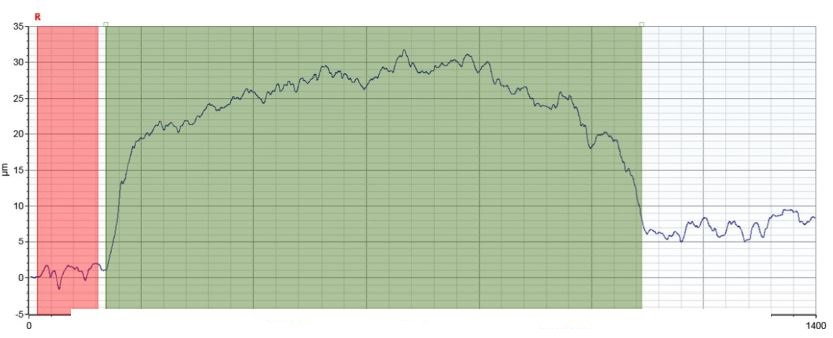
\includegraphics[width=0.8\textwidth]{Figuras/Figura_grafico_perfilometro}
  \caption{Gráfico de caracterización del espesor.}
  \label{fig:Figura_grafico_perfilometro}
\end{figure}

Para los mencionados estudios se utilizaron dos muestras, identificadas como cartuchos nPoc3 y nPoc5, teniendo dos capas curadas de 1 mm y 1,1 mm de diámetro (Tinta de nanopartículas de oro) respectivamente. De cada uno de ellos se utilizaron los electrodos de trabajo identificados como 3 y 4 para obtener un muestreo variado. Se realizaron dos mediciones sobre cada uno y luego se promediaron.

\subsection{Caracterización electroquímica}
La caracterización electroquímica se realizó sobre diferentes configuraciones de sustratos y tintas para obtener múltiples comparaciones de interés para el proyecto. Se listan las muestras por orden de prueba (Figura ~\ref{fig:Figura_pruebas_muestras}):

$\bullet$ Electrodo de película delgada de oro depositado por \textit{sputtering} sobre silicio. (Figura ~\ref{fig:Figura_pruebas_muestras} (a))

$\bullet$ Electrodo de película impresa con carbono por serigrafía sobre sustrato \textit{Valox}. (Figura ~\ref{fig:Figura_pruebas_muestras} (b))

$\bullet$ Electrodo de película impresa con tinta de carbono por serigrafía y con impresión de tinta de nanopartículas de oro de 1 mm de diámetro sobre sustrato \textit{Valox}. (Figura ~\ref{fig:Figura_pruebas_muestras} (c))

$\bullet$ Electrodo de película impresa con tinta de carbono por serigrafía y con impresión de tinta de nanopartículas de oro de 1,1 mm de diámetro sobre sustrato \textit{Valox}.

$\bullet$ Impresión de tinta de nanopartículas de oro sobre sustrato \textit{Valox}.

$\bullet$ Impresión de tinta de nanopartículas de oro sobre sustrato PET. (Figura ~\ref{fig:Figura_pruebas_muestras} (d))

$\bullet$ Impresión de tinta de nanopartículas de oro sobre sustrato de pulpa de celulosa. (Figura ~\ref{fig:Figura_pruebas_muestras} (e))

\begin{figure}[H]
  \centering
    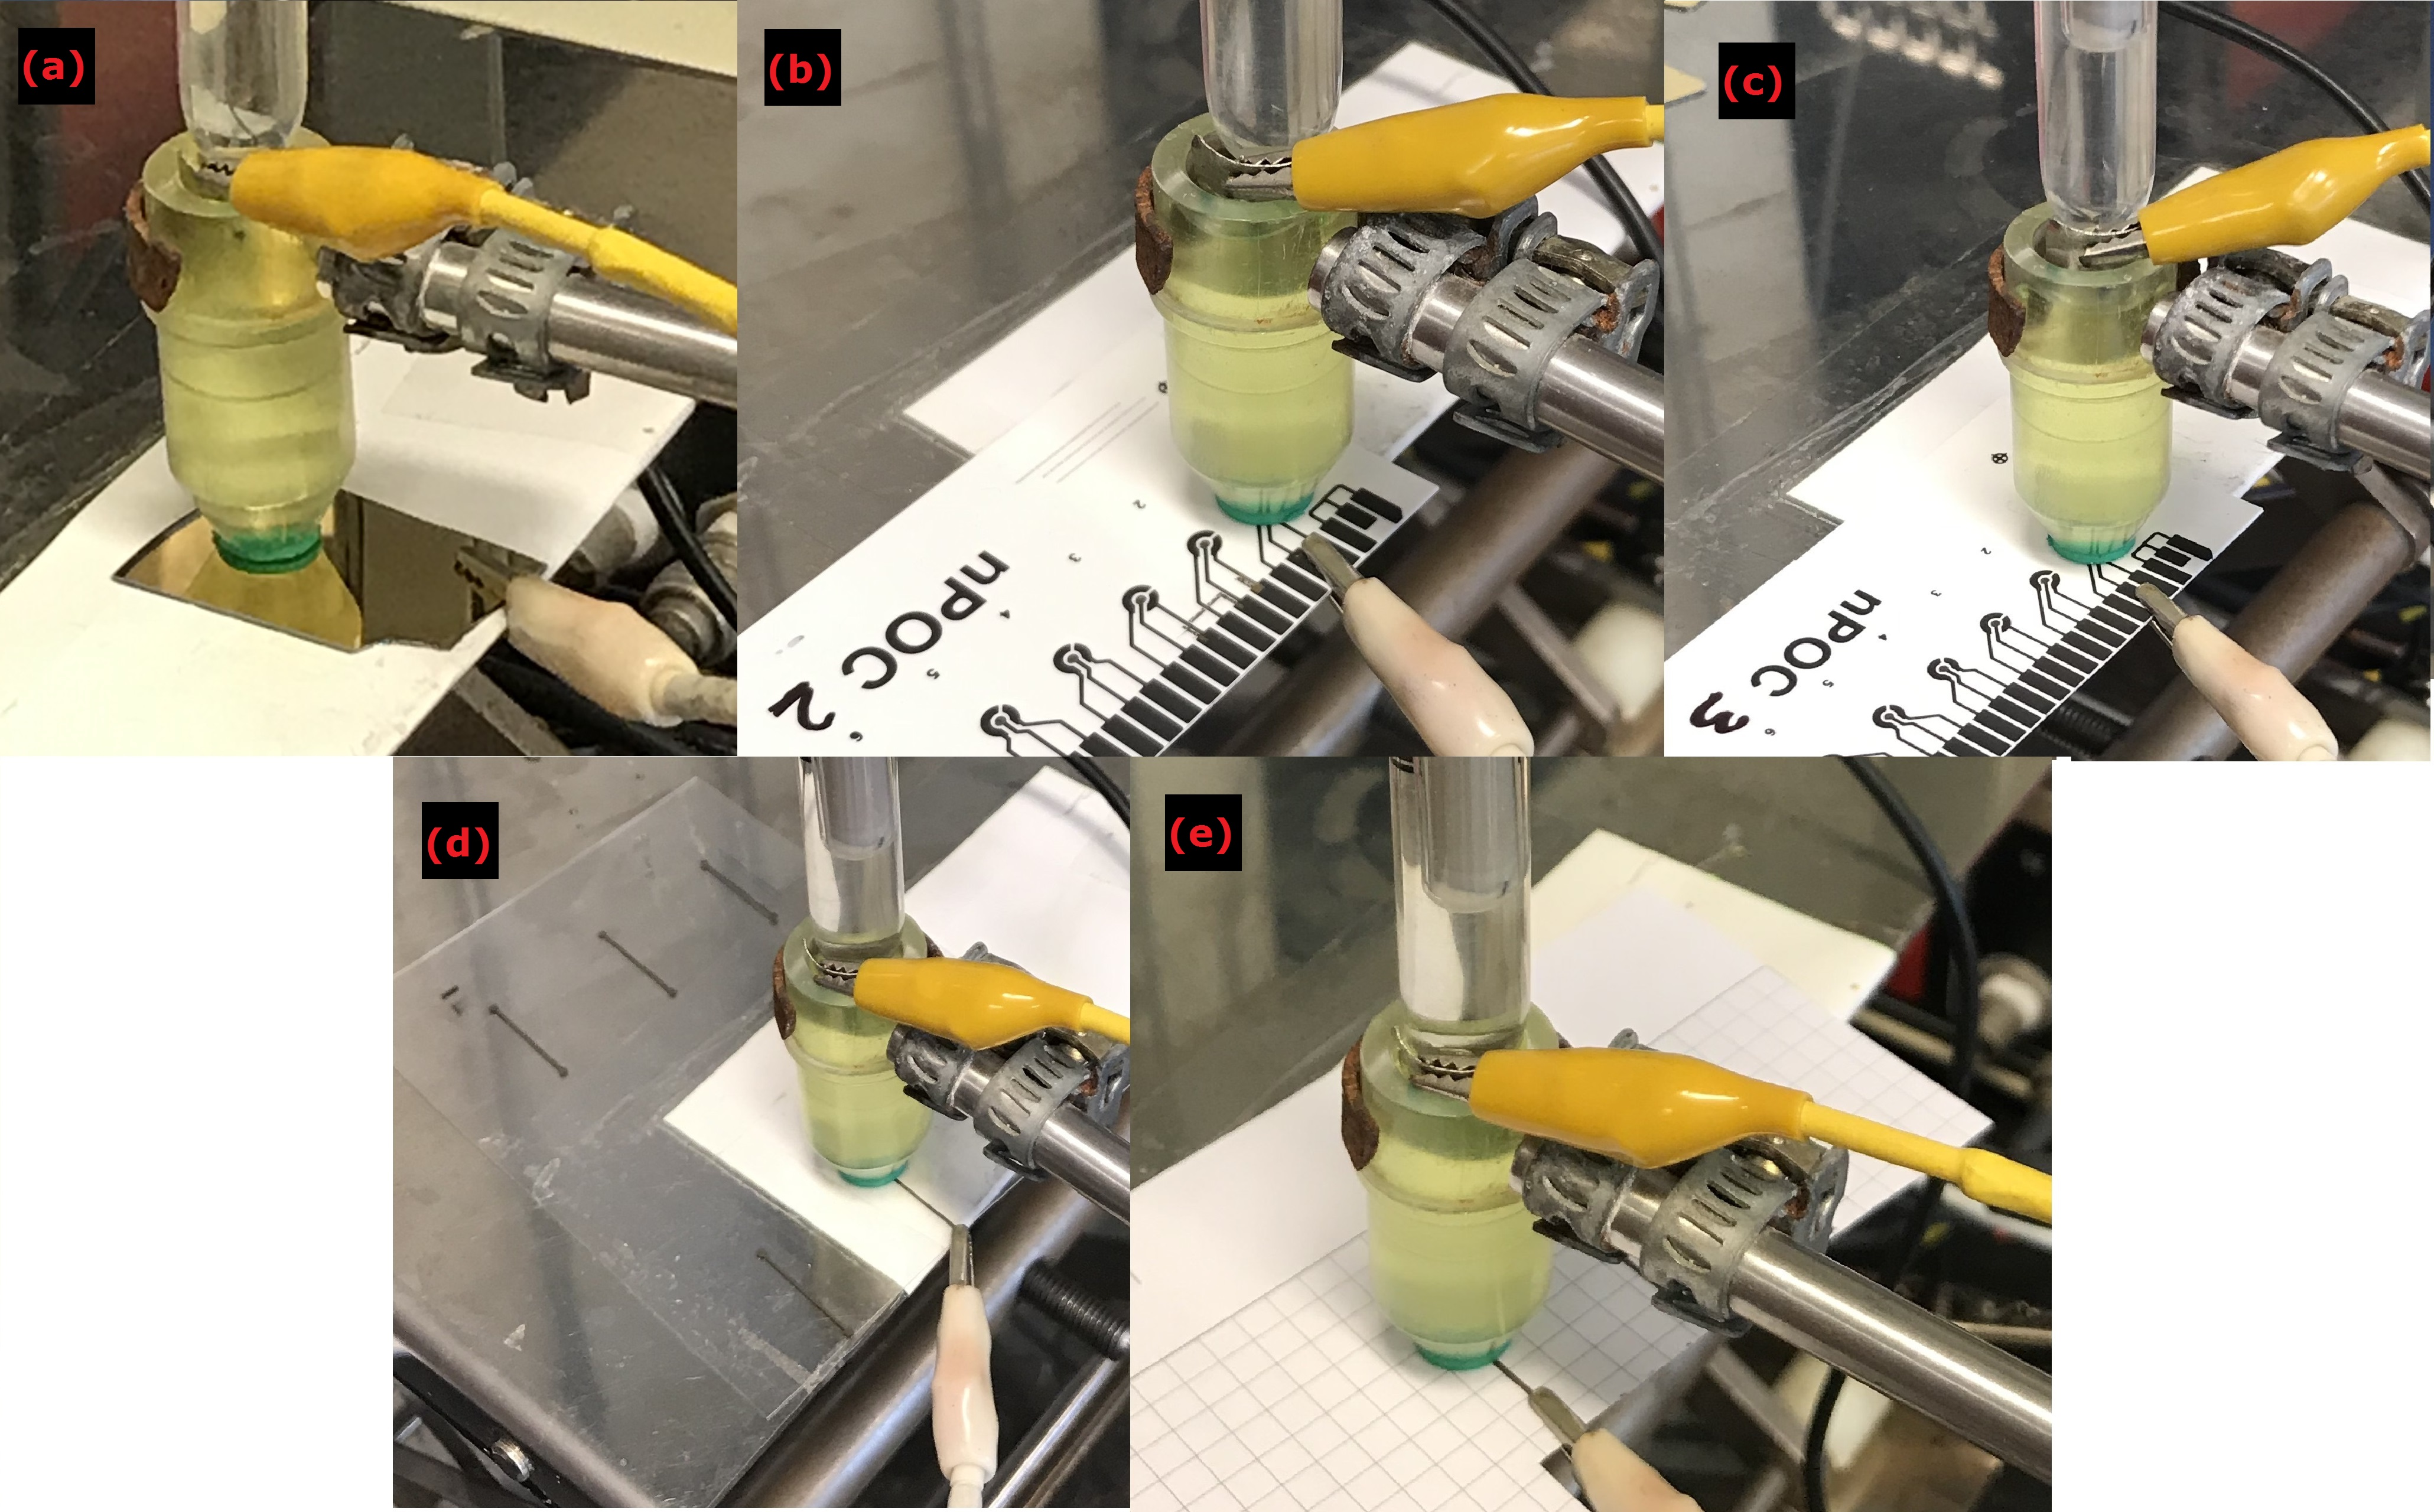
\includegraphics[width=1\textwidth]{Figuras/Figura_pruebas_muestras}
  \caption{Muestras donde se realizó la caracterización electroquímica.}
  \label{fig:Figura_pruebas_muestras}
\end{figure}

Para que las pruebas sean comparables entre sí, se utilizó un contraelectrodo de platino de 2 cm\textsuperscript{2} de área y un electrodo de referencia de cloruro de mercurio(I) o \textit{Calomel} saturado de la firma \textit{Cole-Parmer} (Hg\textsubscript{2}Cl\textsubscript{2}), ambos externos a las muestras. El reservorio de la celda electroquímica fue fabricada en acrílico con un volumen aproximado de 3 ml. Posee un orificio en la parte inferior donde pueden colocarse sellos de polipropileno. En los experimentos se utilizó un sello de 1 mm de diámetro, para tener el mismo área geométrica de 0,785 mm\textsuperscript{2} en todas las pruebas.

Luego de poner en contacto el sello con el electrodo se llena la celda por la parte superior con la solución sonda de ferrocianuro (K\textsubscript{4}Fe(CN)\textsubscript{6}), ferricianuro (K\textsubscript{3}Fe(CN)\textsubscript{6}) y el electrolito soporte cloruro de potasio (KCl). Se verificó que no hubiera pérdidas de líquido (Figura ~\ref{fig:Figura_prueba_electroquimica}).

\begin{figure}[H]
  \centering
    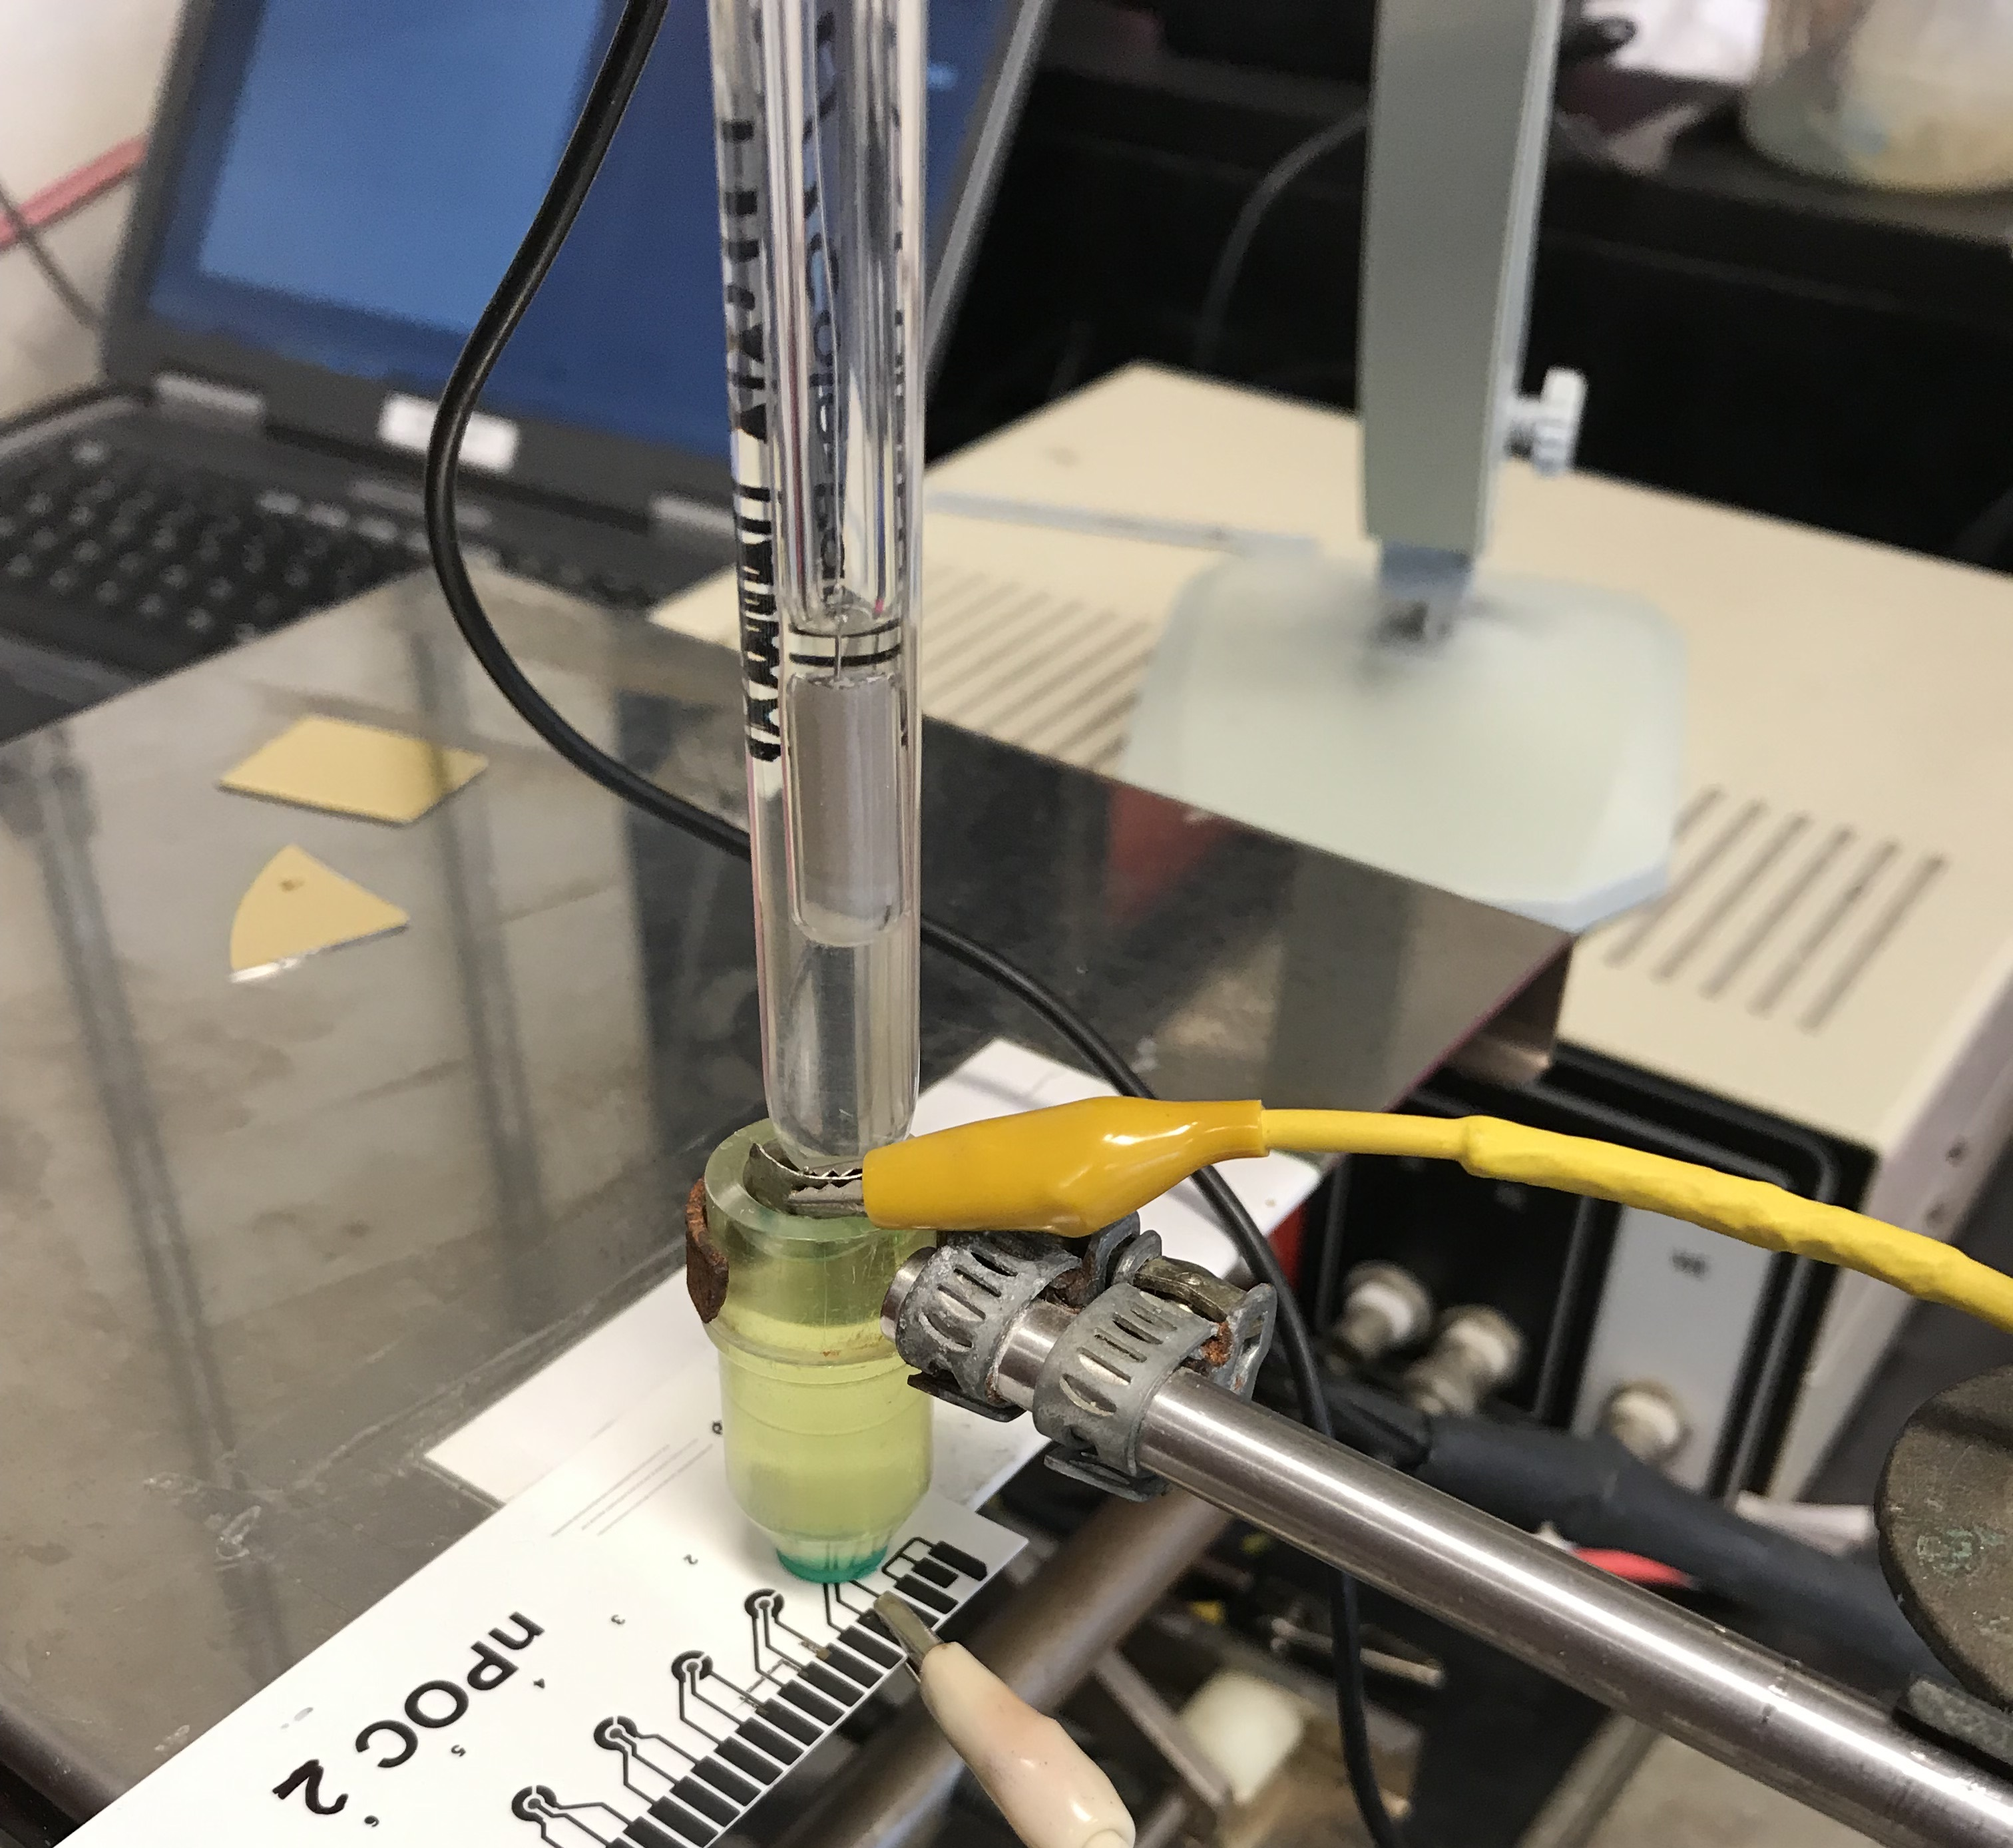
\includegraphics[width=0.5\textwidth]{Figuras/Figura_prueba_electroquimica}
  \caption{Arreglo experimental para mediciones electroquímicas.}
  \label{fig:Figura_prueba_electroquimica}
\end{figure}

Se debe tener especial cuidado para que el sello no obstruya parte del electrodo de trabajo, de lo contrario el mismo no estará completamente cubierto por la solución sonda (Figura ~\ref{fig:Figura_electrodo_sonda}). Además, se debe comprobar que al llenar la cubeta no se formen burbujas, ya que tampoco se cubriría por completo el electrodo de trabajo.

\begin{figure}[H]
  \centering
    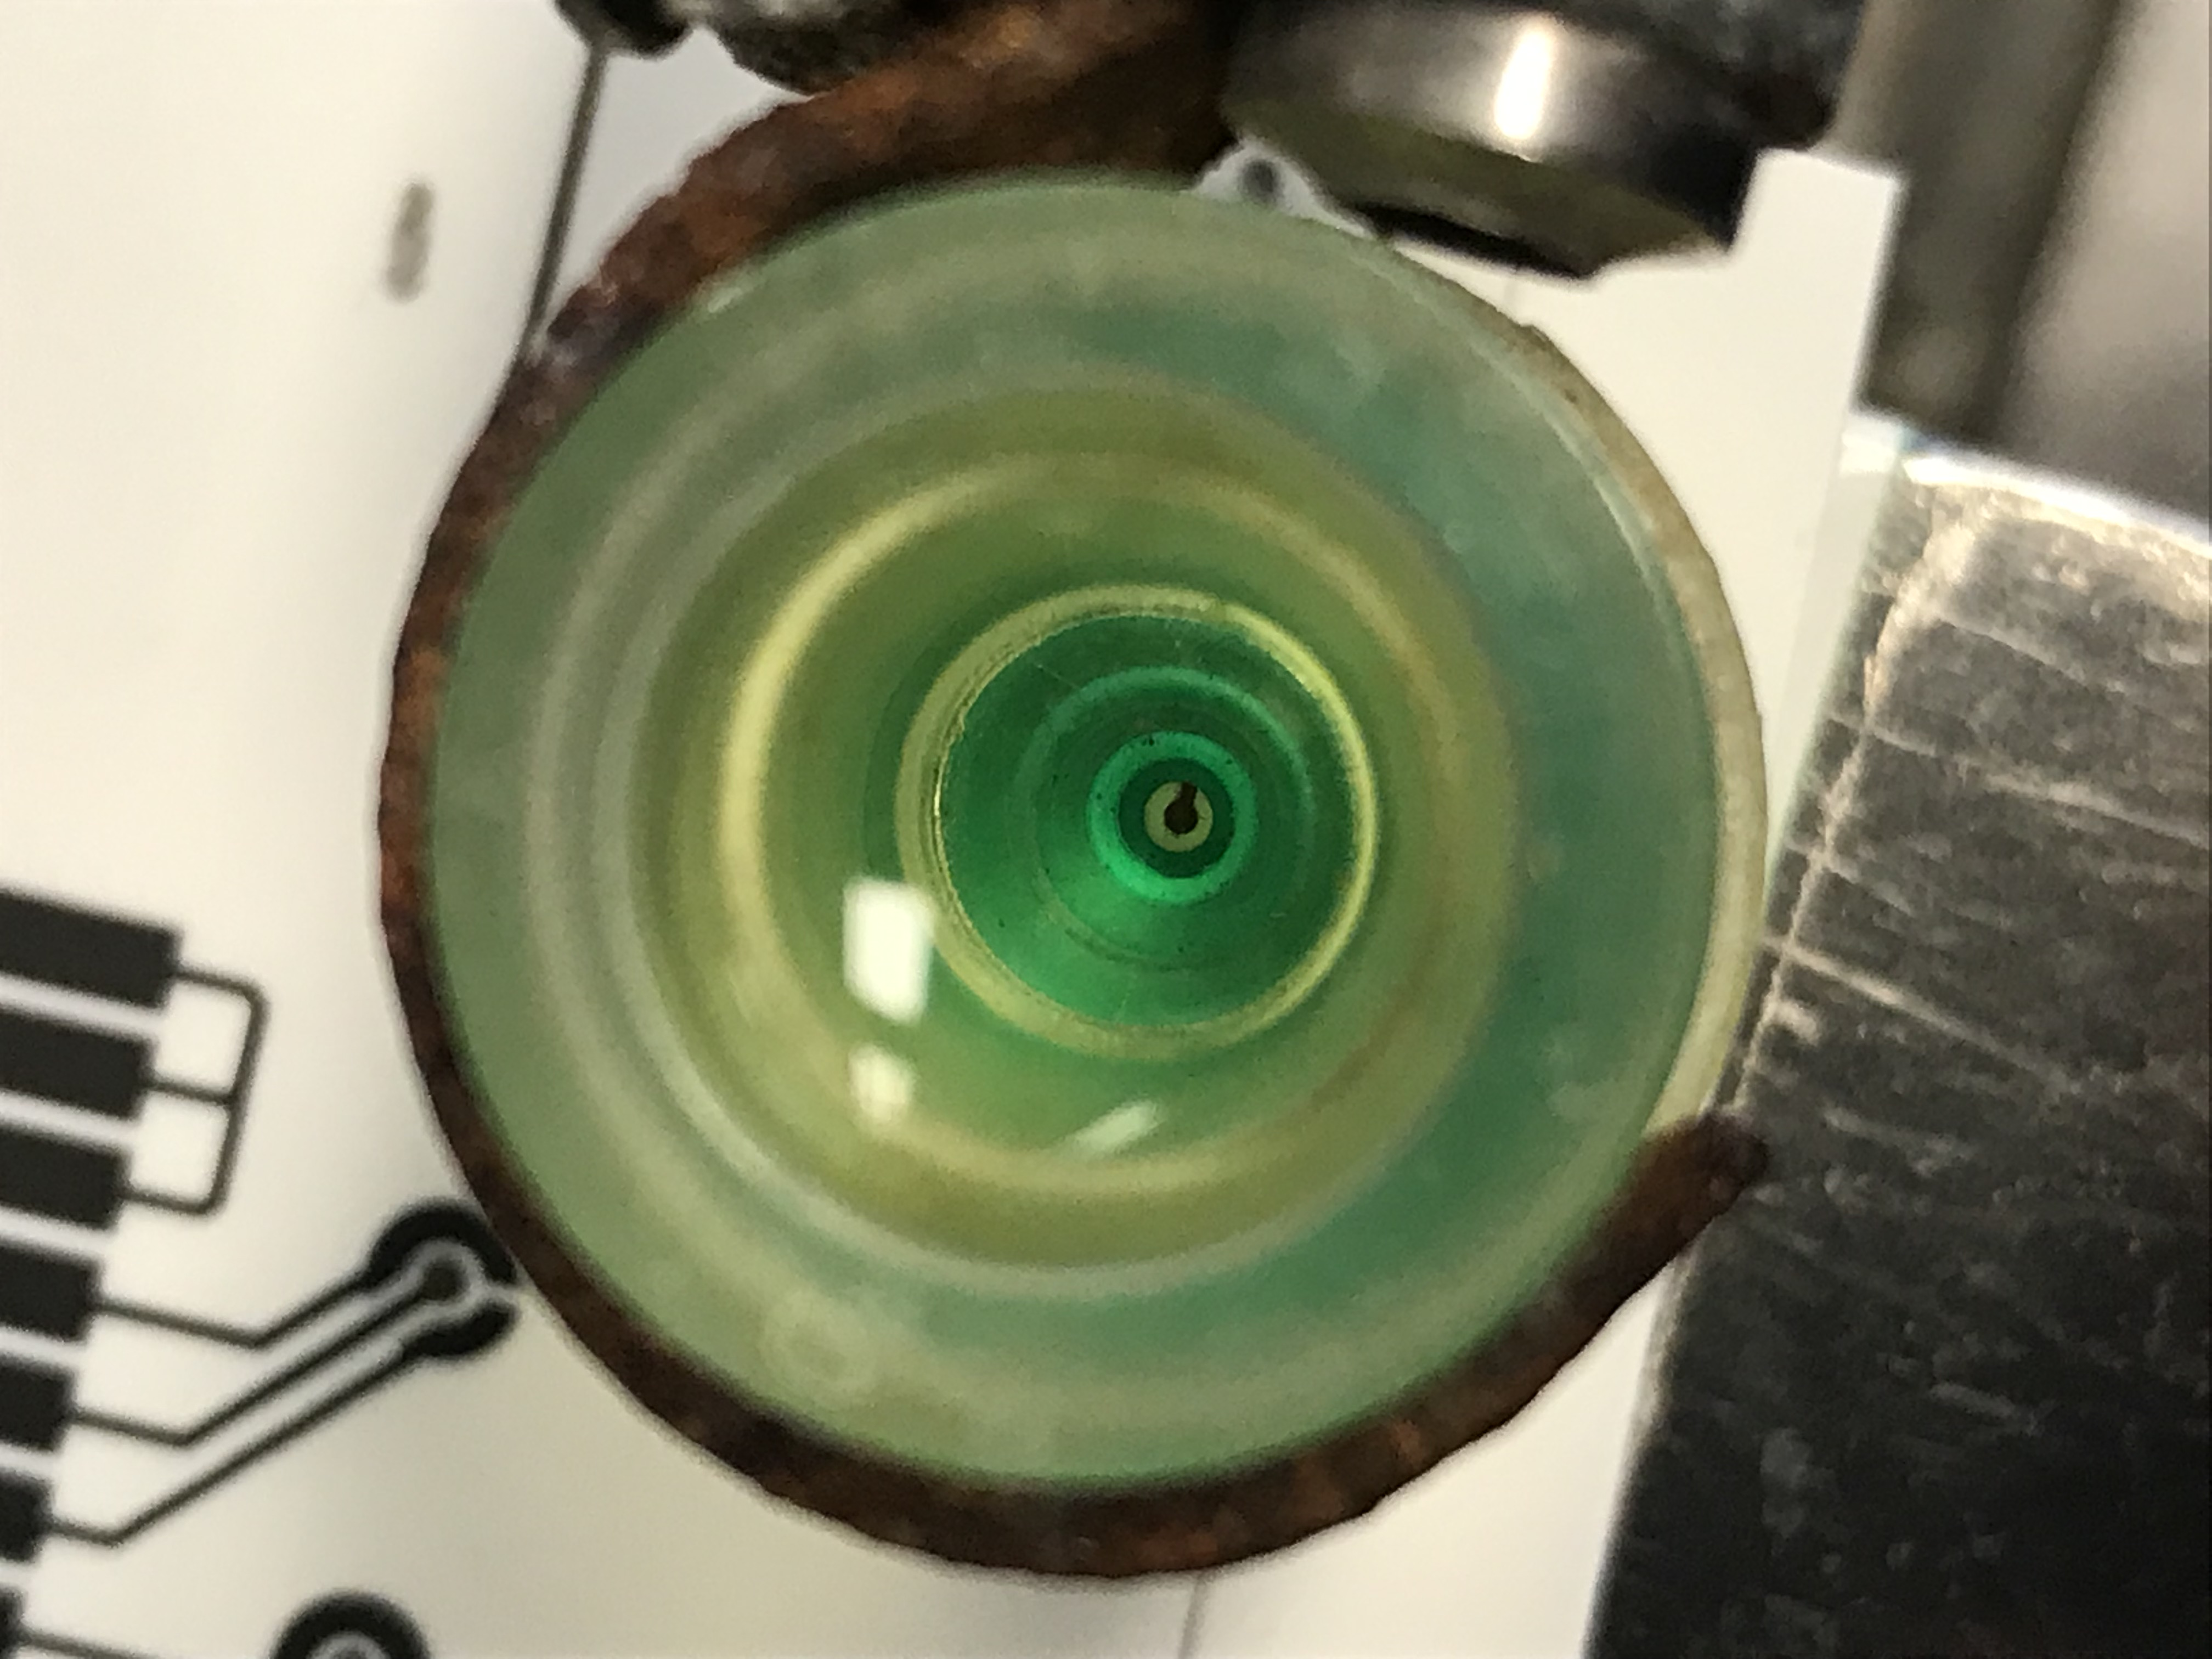
\includegraphics[width=0.5\textwidth]{Figuras/Figura_electrodo_sonda}
  \caption{Electrodo en celda de acrílico.}
  \label{fig:Figura_electrodo_sonda}
\end{figure}

Las mediciones fueron tomadas con un potenciostato marca \textit{Teq4}. La señal de excitación es un barrido de potencial lineal con una forma de onda triangular de potencial mínimo E1 (-200 mV) y un potencial máximo E2 (500 mV), con una velocidad de barrido de 50 mV·s\textsuperscript{-1}. Utilizando el software del potenciostato se tomaron los datos de tensiones y corrientes y se exportaron en formato \textit{valores separados por comas} (CSV) para ser procesados posteriormente en software de código libre \textit{GNUplot}. Además, se guardaron en formato PNG los gráficos realizados por el software del potenciostato para tener como referencia (Figura ~\ref{fig:Figura_software_potenciostato}).

\begin{figure}[H]
  \centering
    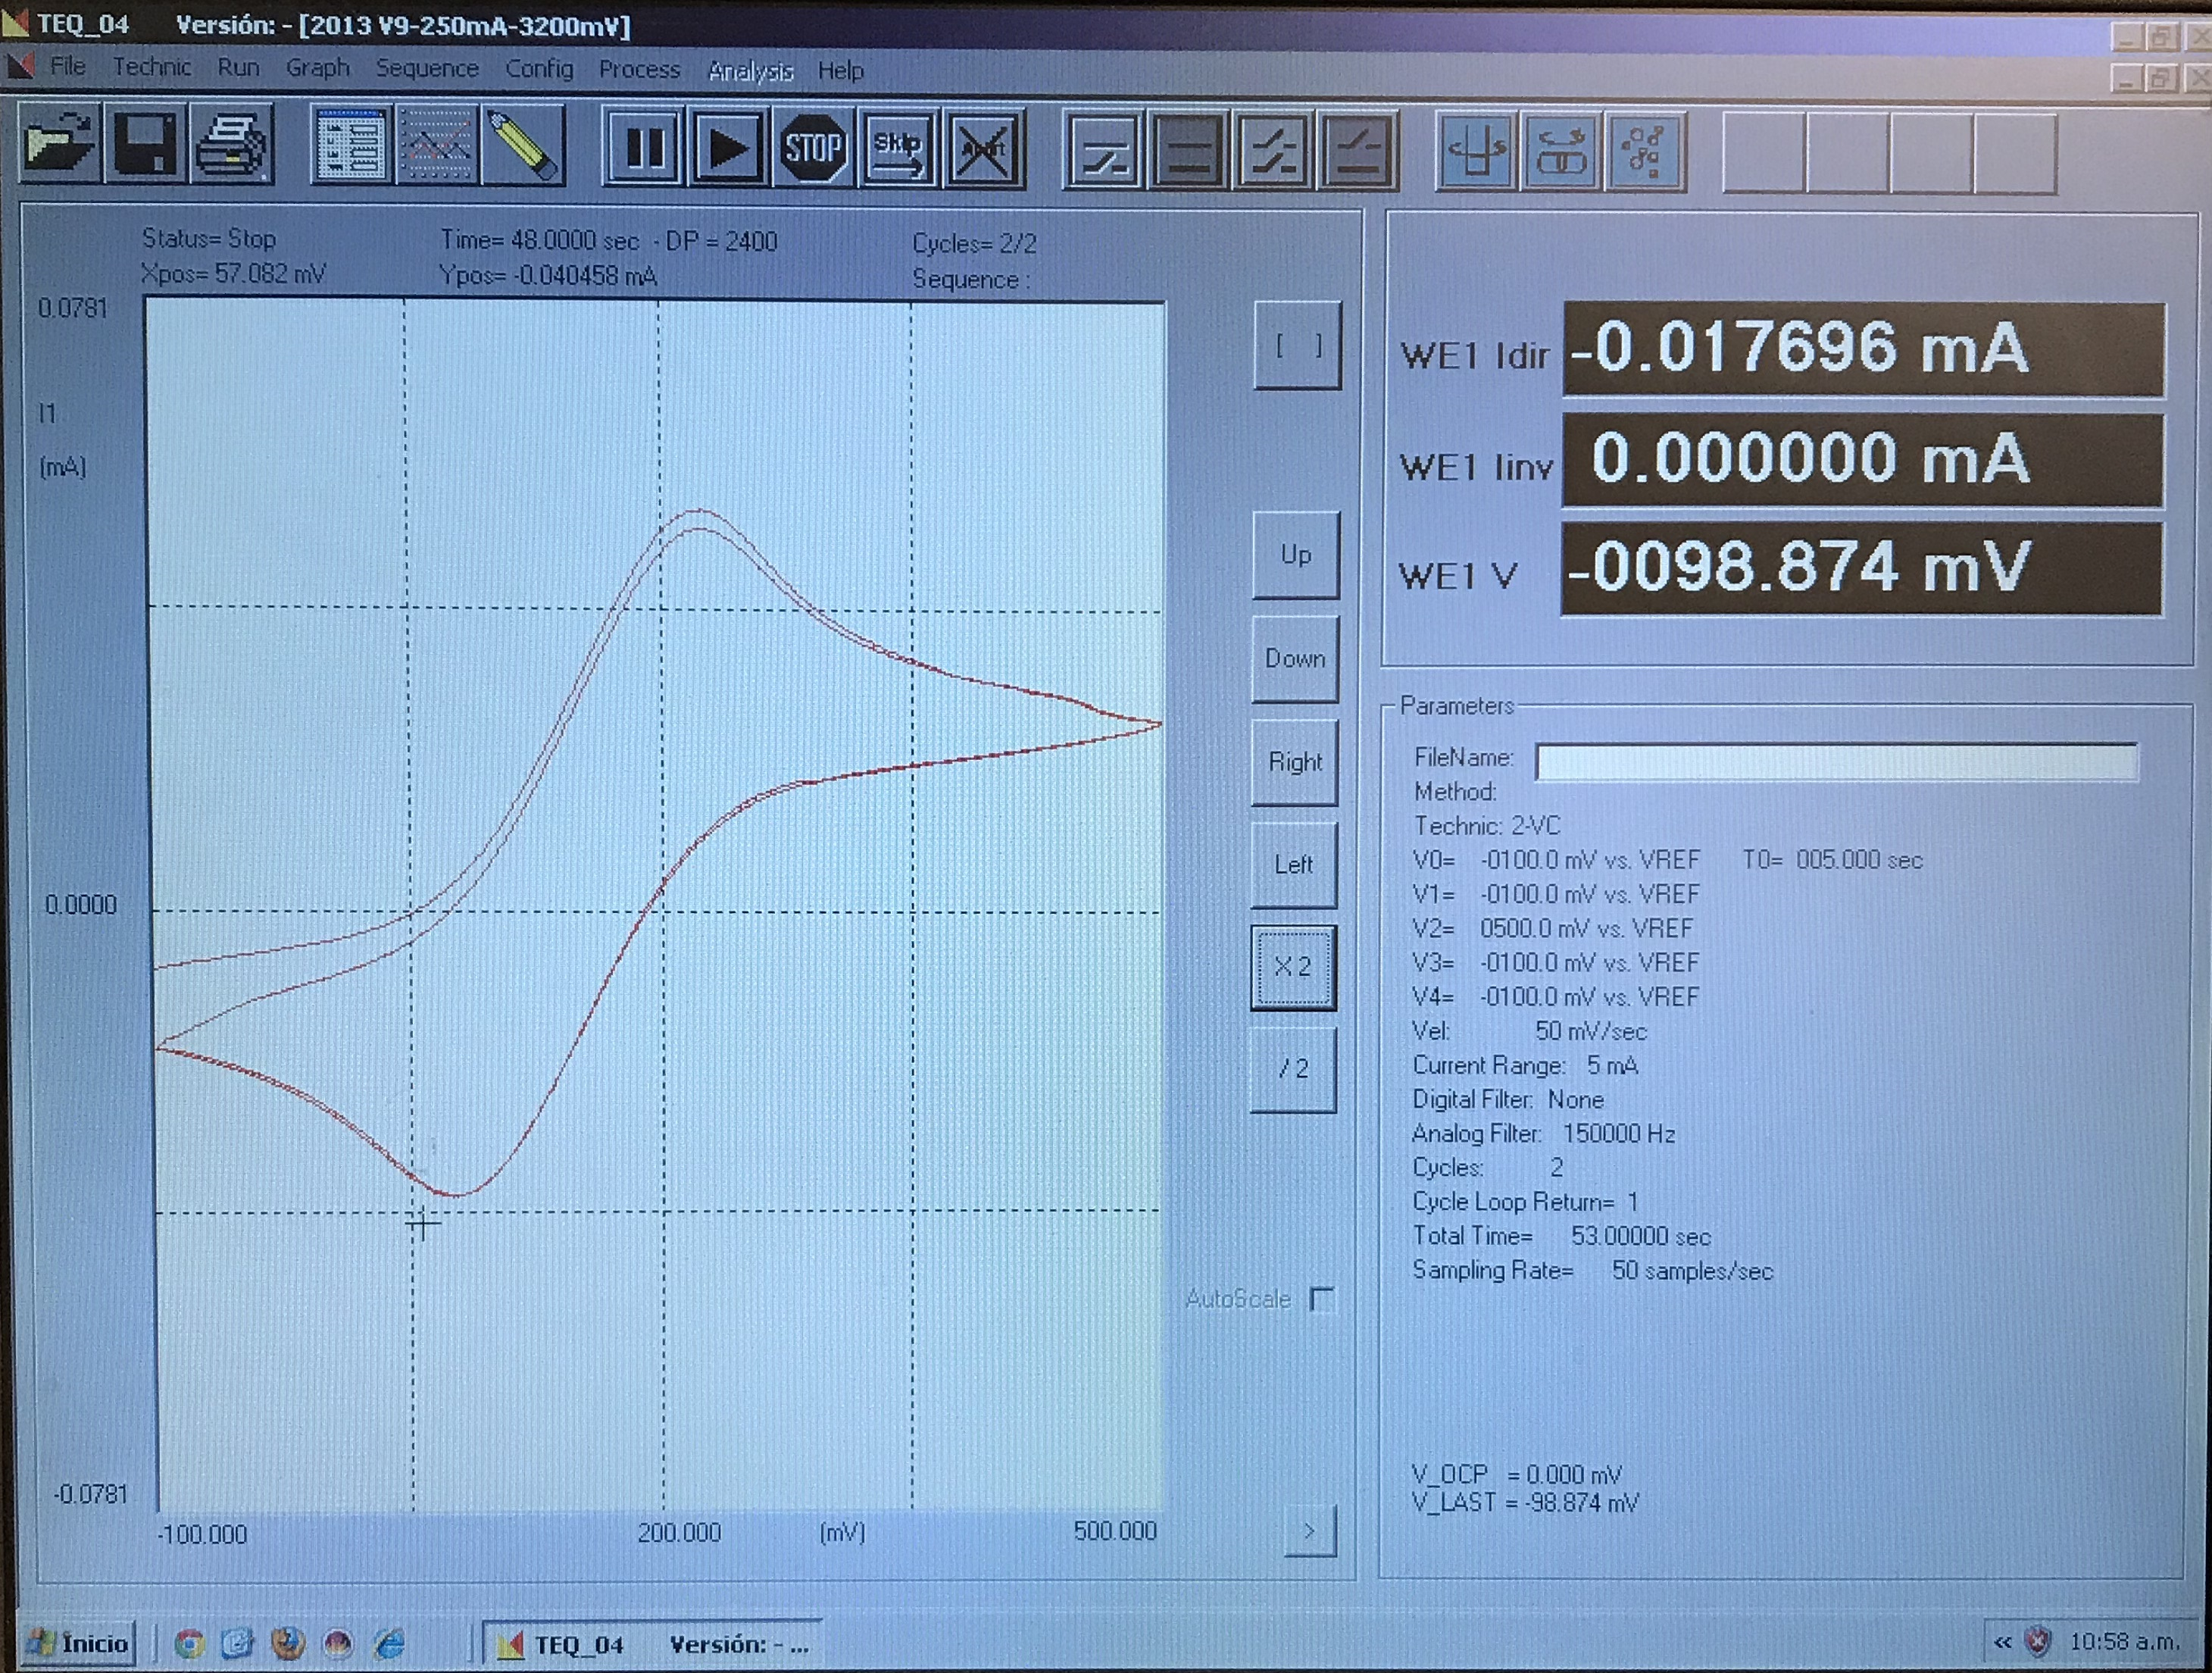
\includegraphics[width=0.5\textwidth]{Figuras/Figura_software_potenciostato}
  \caption{Software de potenciostato \textit{Teq4} con gráfico de medición.}
  \label{fig:Figura_software_potenciostato}
\end{figure}

Una vez realizados los experimentos sobre todas las muestras, se procesaron los datos para conocer los resultados y conclusiones del proyecto.

\section{Tinta dieléctrica fotorresistente}\label{sec:tinta_dielec}
En esta sección se dejará planteado un proyecto a continuar, como paso siguiente a la impresión de nanopartículas de oro sobre los electrodos de trabajo. Utilizando la tinta dieléctrica fotorresistente se realizarán microcubetas alrededor de los \emph{WE}. Para generar estas estructuras 3D por impresiones \textit{Inkjet}, se deberán imprimir varias capas con sus respectivos curados, formando un cilindro centrado sobre cada uno de los ocho \emph{WE}. De esta manera, se busca formar un contenedor por cada celda electroquímica, donde se inyectarán las muestras a analizar. La principal ventaja por la que se propone este proyecto es el de utilizar la impresora \textit{Inkjet} para la fabricación completa del biosensor, sin necesidad de utilizar otros procesos.

\subsection{Diseño}
Teniendo las dimensiones de los electrodos de trabajo, se diseñaron 3 anillos de diferentes tamaños como primera aproximación. Estas figuras, impresas en varias capas formarán la microcubeta que mantendrá la muestra contenida sobre la celda electroquímica. Las dimensiones de los diseños fueron de 1050, 1100 y 1150 $\mu$m de radio interior y 1350, 1300 y 1250 $\mu$m de radio externo, respectivamente. (Figura ~\ref{fig:Figura_anillos_SU8}).

\begin{figure}[H]
  \centering
    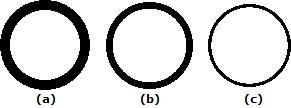
\includegraphics[width=0.5\textwidth]{Figuras/Figura_anillos_SU8}
  \caption{(a) Anillo de 1050 a 1350 $\mu$m. (b) Anillo de 1100 a 1300 $\mu$m. (c) Anillo de 1150 a 1250 $\mu$m.}
  \label{fig:Figura_anillos_SU8}
\end{figure}

De esta forma se obtienen anillos de 100, 200 y 300 $\mu$m de espesor, con los cuales se determinarán los valores óptimos para la impresión de varias capas sucesivas, formando la microcubeta.

\subsection{Preparación de cartucho de tinta}
Para la formulación de la tinta se utilizó una resina llamada \textit{SU-8 2007} como soluto y Ciclohexanona como solvente (Figura ~\ref{fig:Figura_SU8_Ciclohexanona}). Para obtener la viscosidad adecuada para formar y eyectar las gotas de tinta, se calculó la proporción necesaria de cada compuesto. Se determinó que son necesarios 2 ml de Ciclohexanona cada 3 ml de \textit{SU-8 2007}.

\begin{figure}[H]
  \centering
    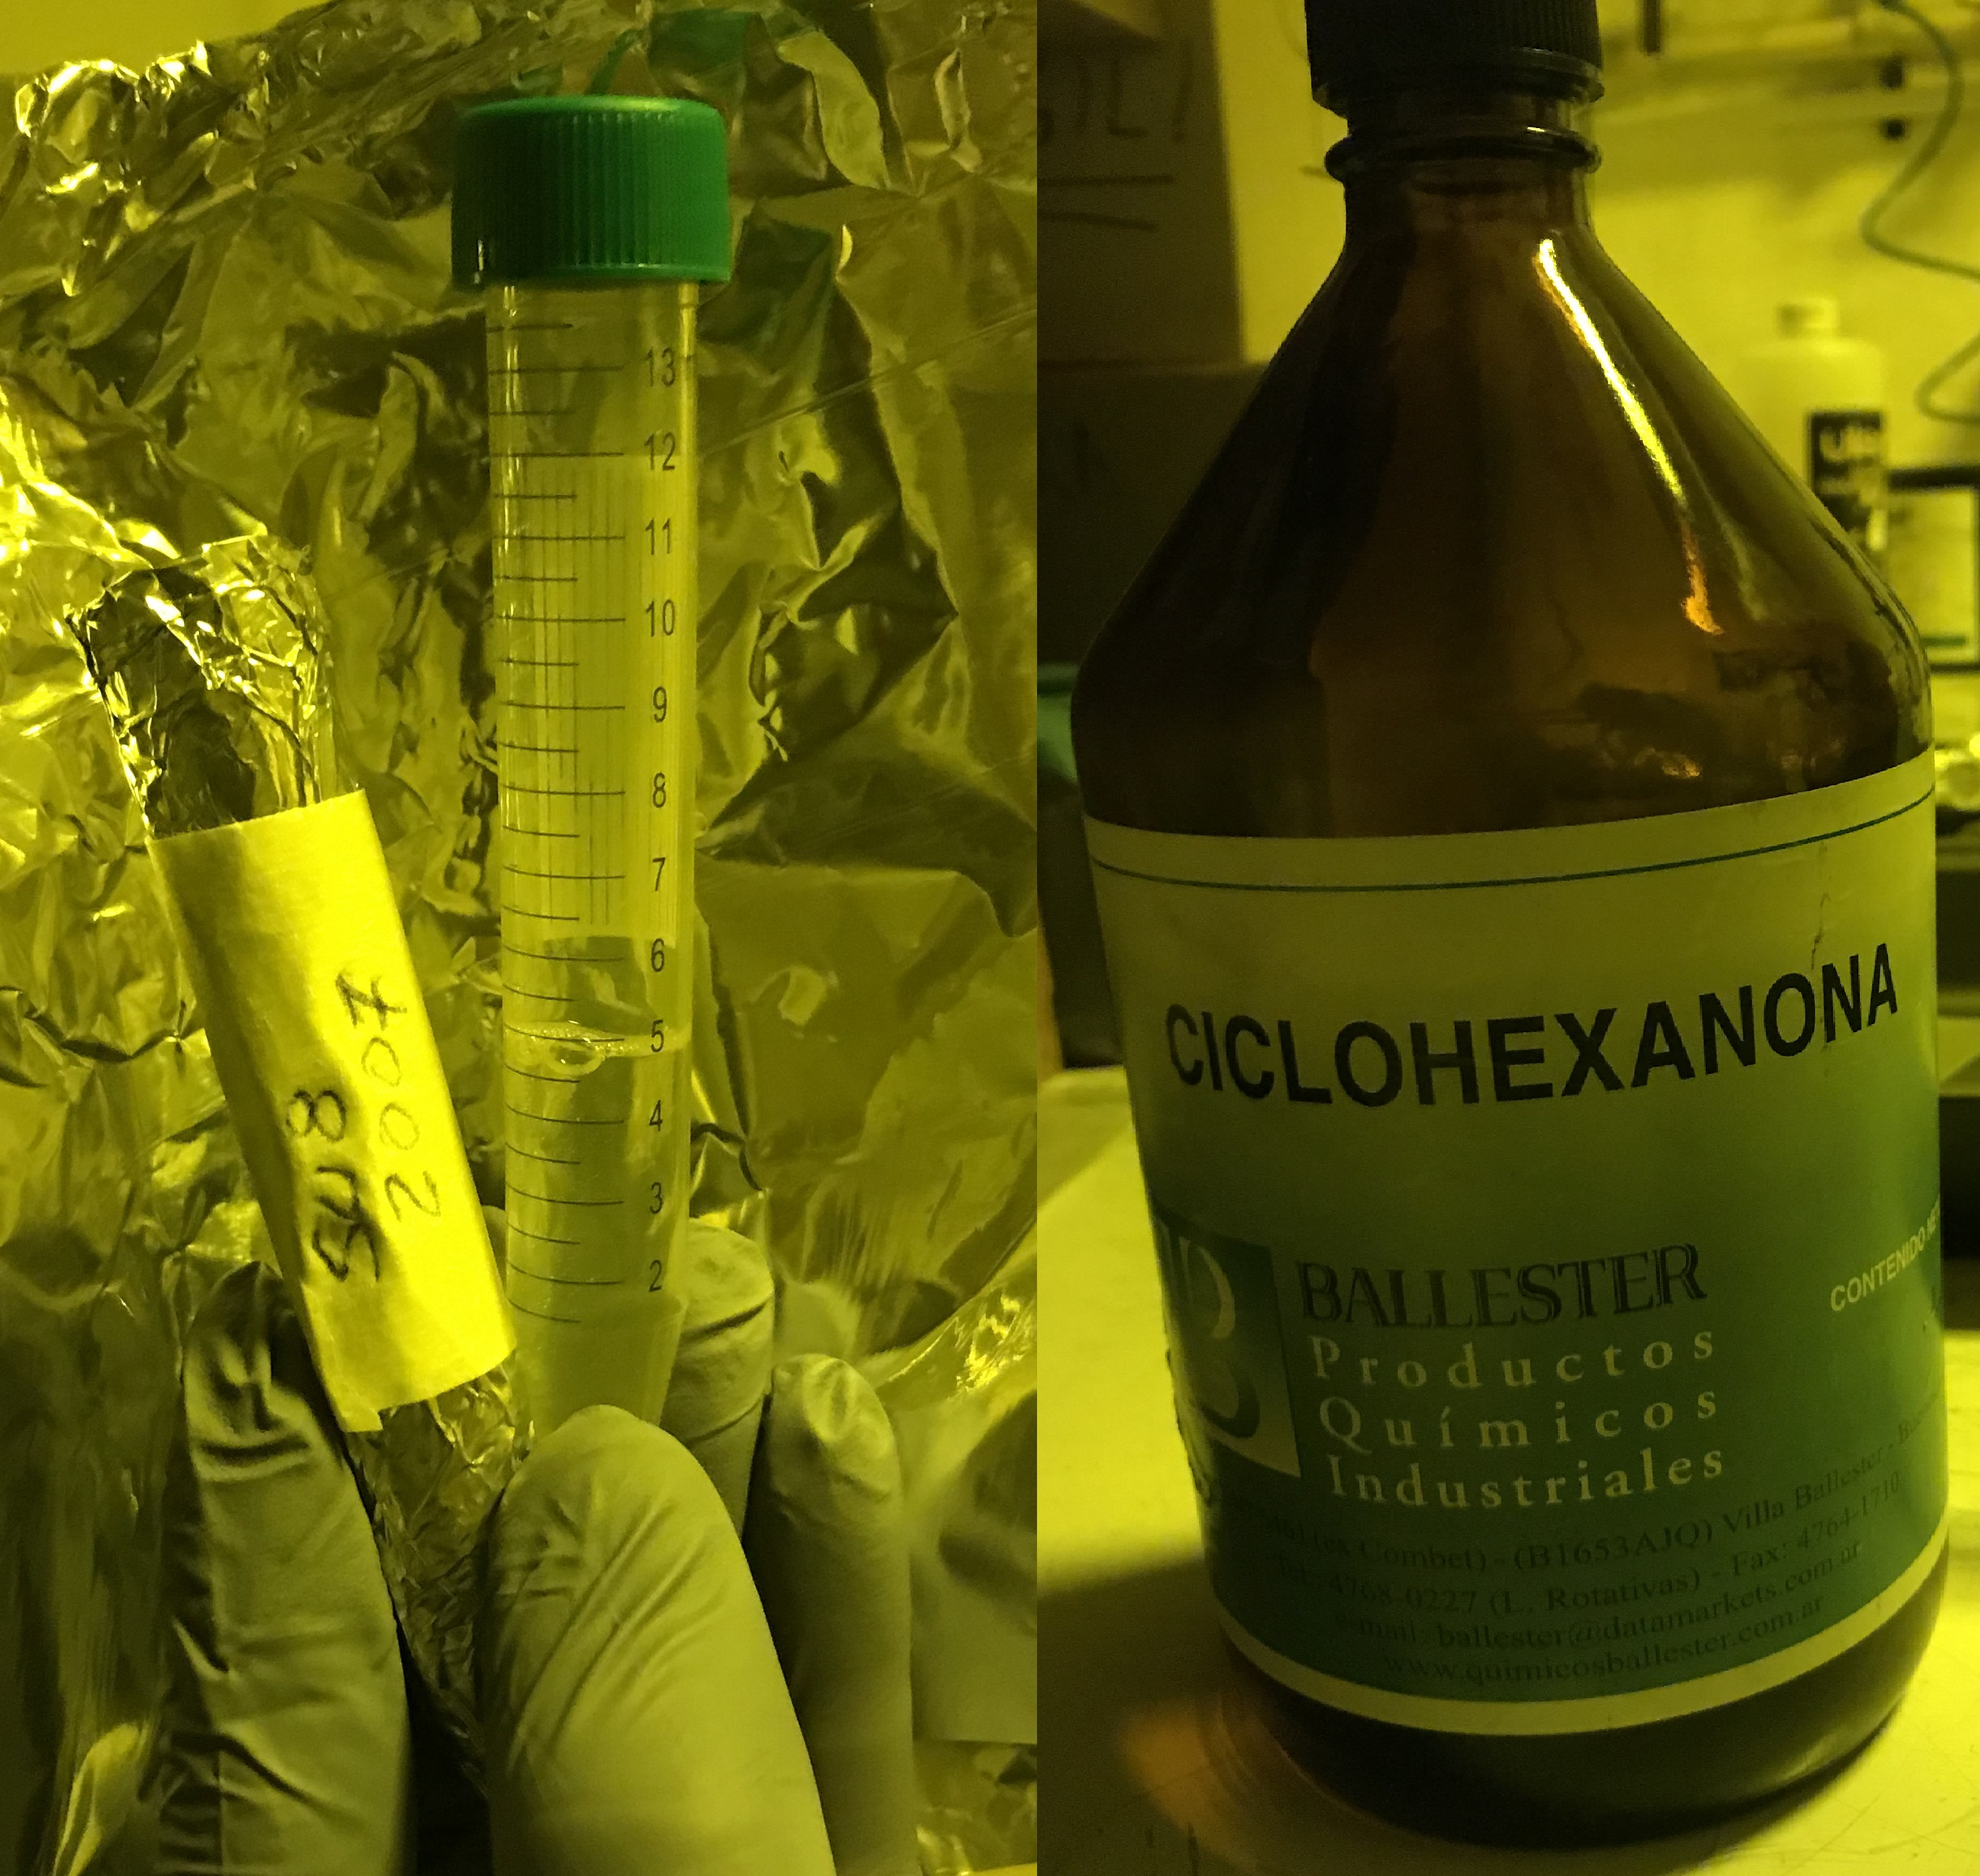
\includegraphics[width=0.5\textwidth]{Figuras/Figura_SU8_Ciclohexanona}
  \caption{Soluto y solvente para formular la tinta dieléctrica fotorresistente.}
  \label{fig:Figura_SU8_Ciclohexanona}
\end{figure}

Dado que dicho soluto es fotosensible, la preparación debió realizarse en una sala oscura con filtros UV. A su vez, el reservorio del cartucho debió protegerse de los rayos UV debido a que la impresora no se encuentra en una sala oscura con los filtros adecuados, lo que secaría la tinta dentro del reservorio. Para esto se utilizó papel de aluminio, formando un cobertor, sin obstaculizar el cabezal y sus conexiones con el carrete (Figura ~\ref{fig:Figura_cartucho_SU8}).

\begin{figure}[H]
  \centering
    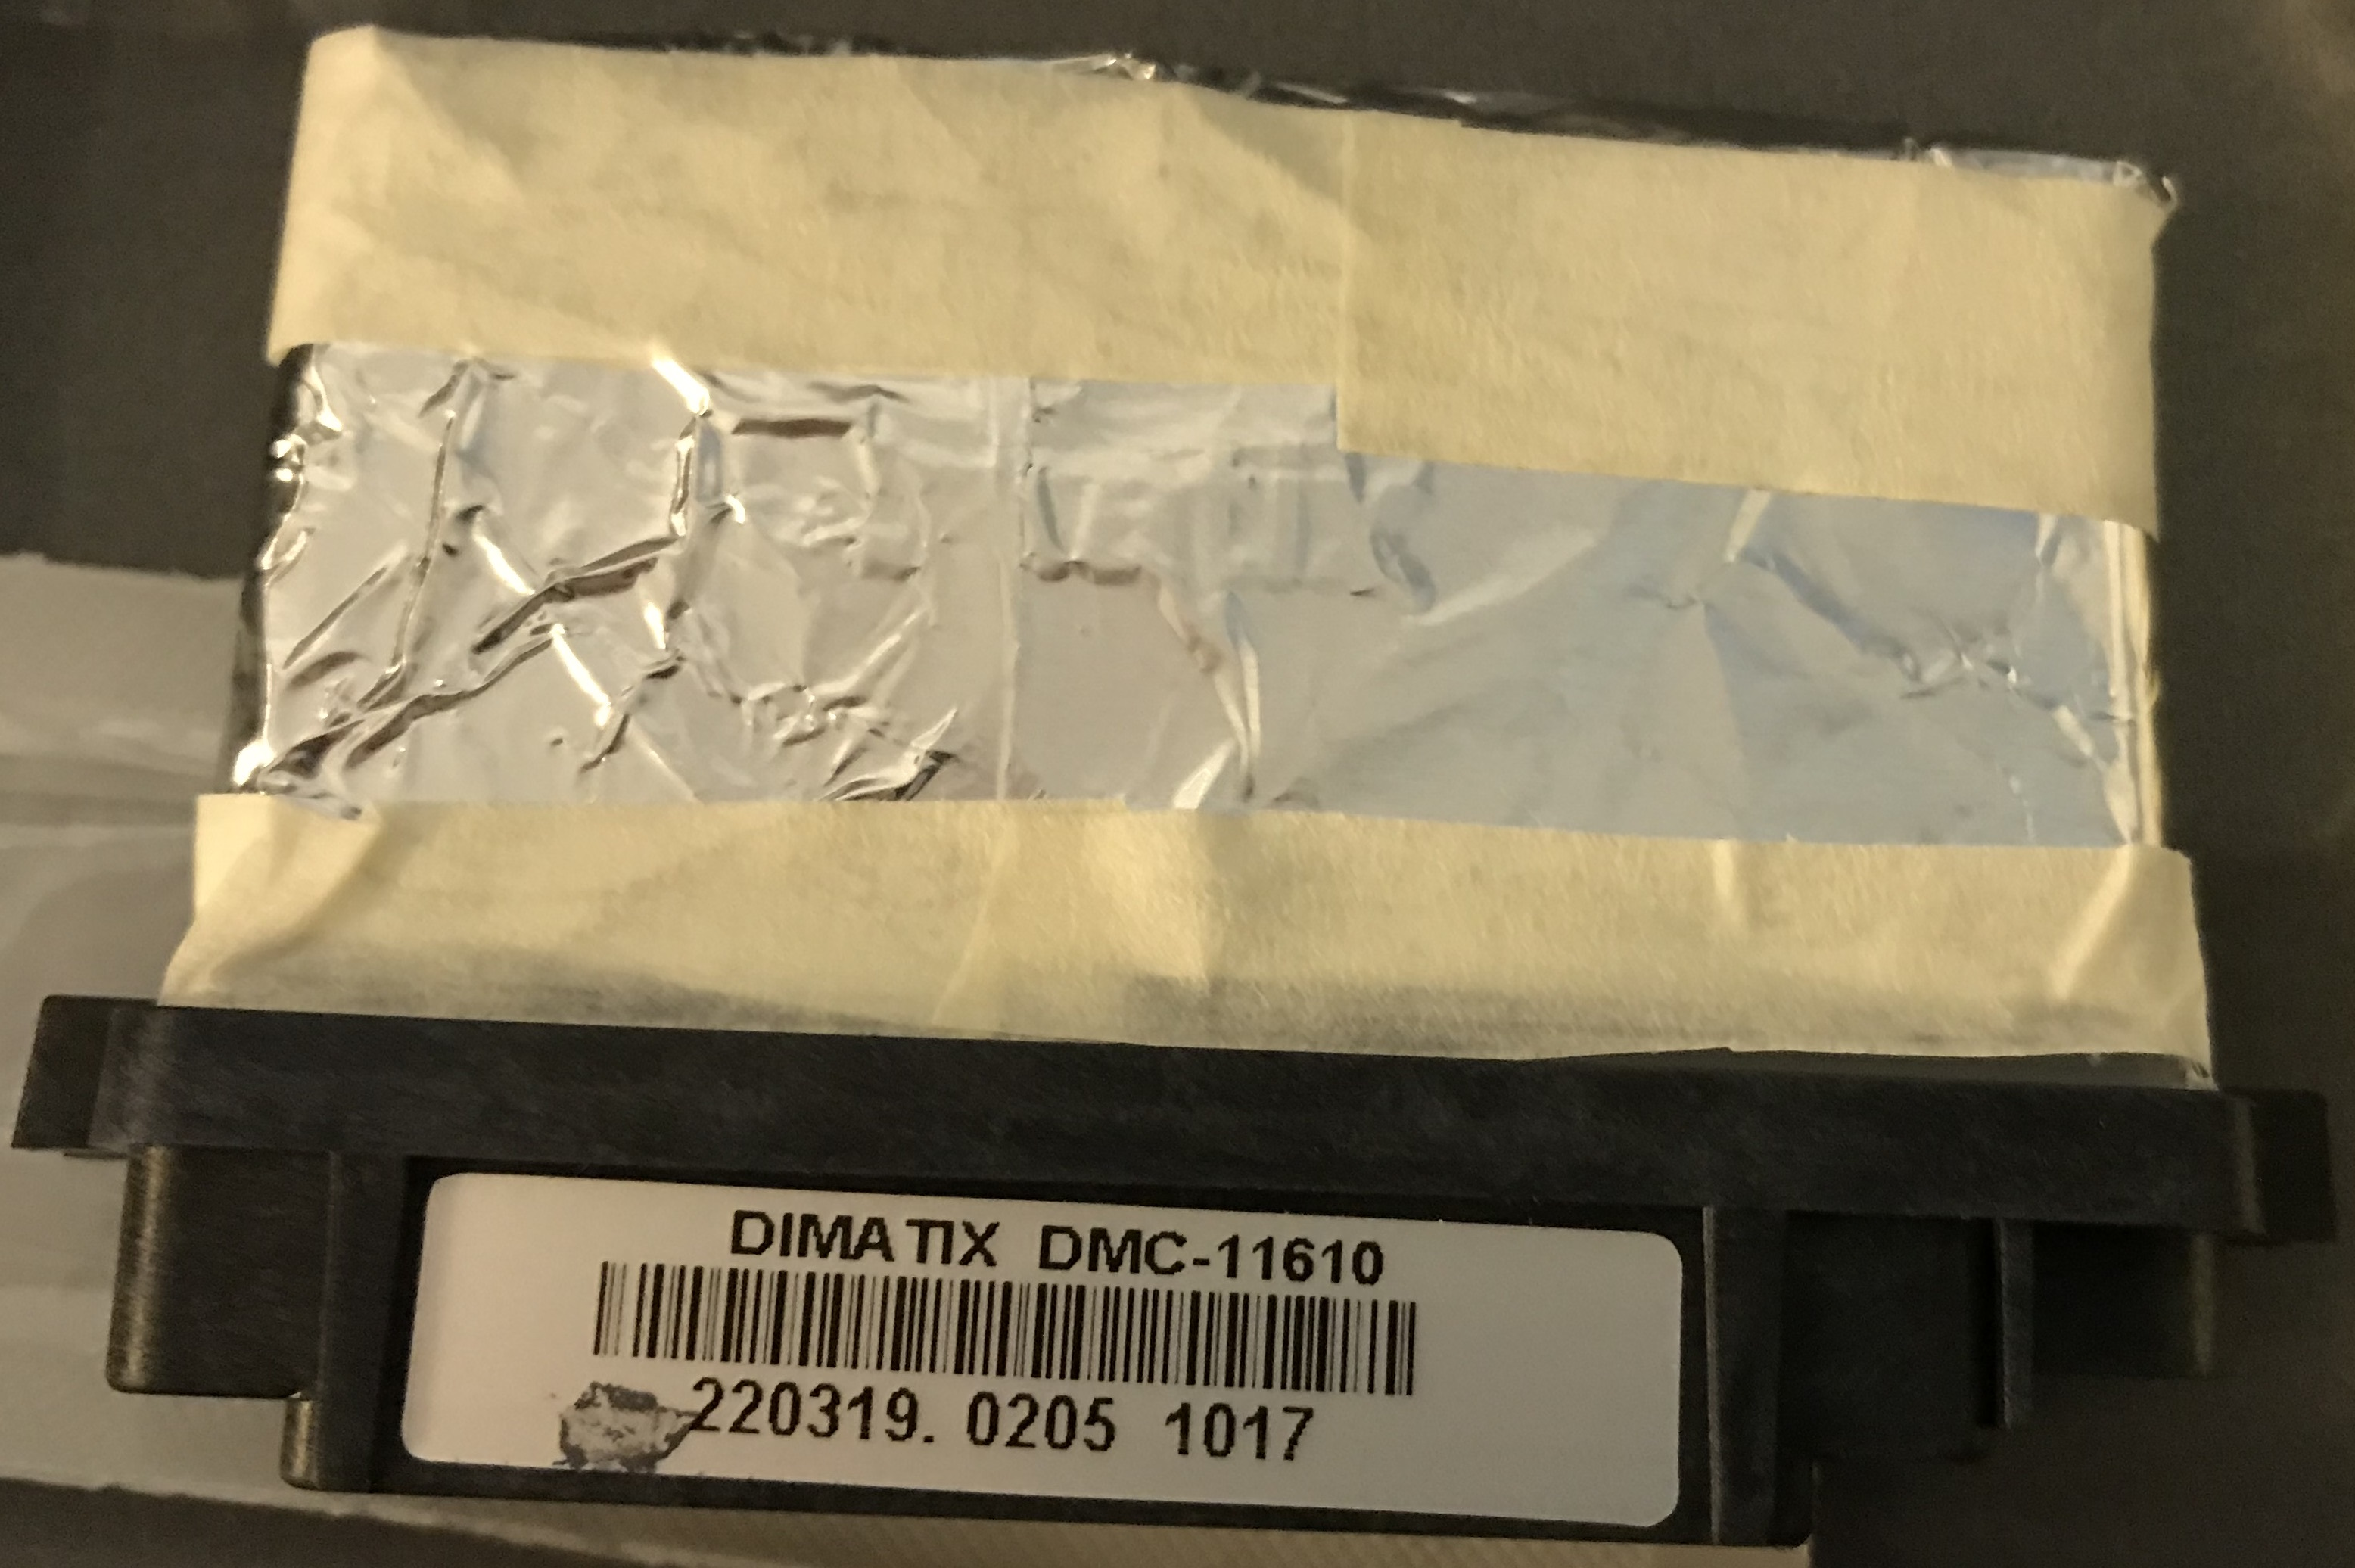
\includegraphics[width=0.5\textwidth]{Figuras/Figura_cartucho_SU8}
  \caption{Cartucho con tinta SU-8 protegido de rayos UV.}
  \label{fig:Figura_cartucho_SU8}
\end{figure}

\subsection{Puesta a punto y calibraci\'on de impresora}
Al instalar el cartucho de tinta en la impresora, se configuraron los parámetros del mismo utilizando la información que provee el fabricante \textit{Microchem} \cite{PriElexSU8}, y se realizaron las primeras pruebas de eyección de tinta en el \textit{Drop Watcher} (Figura ~\ref{fig:Figura_Drop_Watcher_SU8}).

\begin{figure}[H]
  \centering
    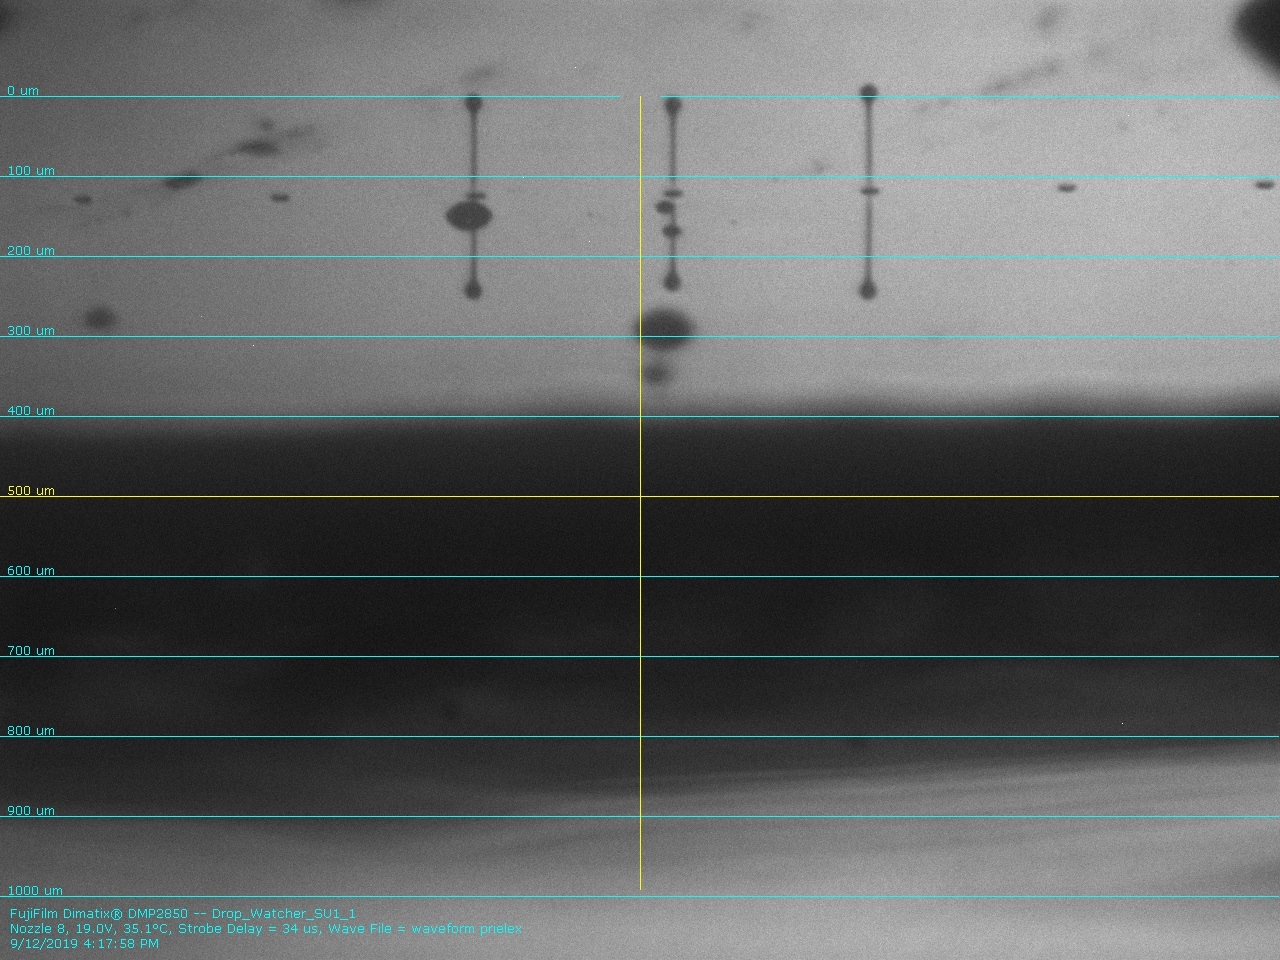
\includegraphics[width=0.5\textwidth]{Figuras/Figura_Drop_Watcher_SU8}
  \caption{Gotas de SU-8 vistas desde la cámara \textit{Drop Watcher}.}
  \label{fig:Figura_Drop_Watcher_SU8}
\end{figure}

Fueron necesarios varios ciclos de purga para obtener la eyección de gotas. Se calibraron las tensiones de los \textit{Nozzles} para tener el mismo tiempo de vuelo entre los 3 eyectores a utilizar.

\subsection{Impresiones}
Se realizó la impresión del archivo $``$\textit{Line Pattern}$"$ para poder definir el espaciado entre gotas necesario para obtener una línea contínua con la tinta \textit{SU-8} sobre sustrato \textit{Valox}. Se definió que el \textit{Drop Spacing} óptimo es de 15 $\mu$m (Figura ~\ref{fig:Figura_LinePattern_SU8}).

\begin{figure}[H]
  \centering
    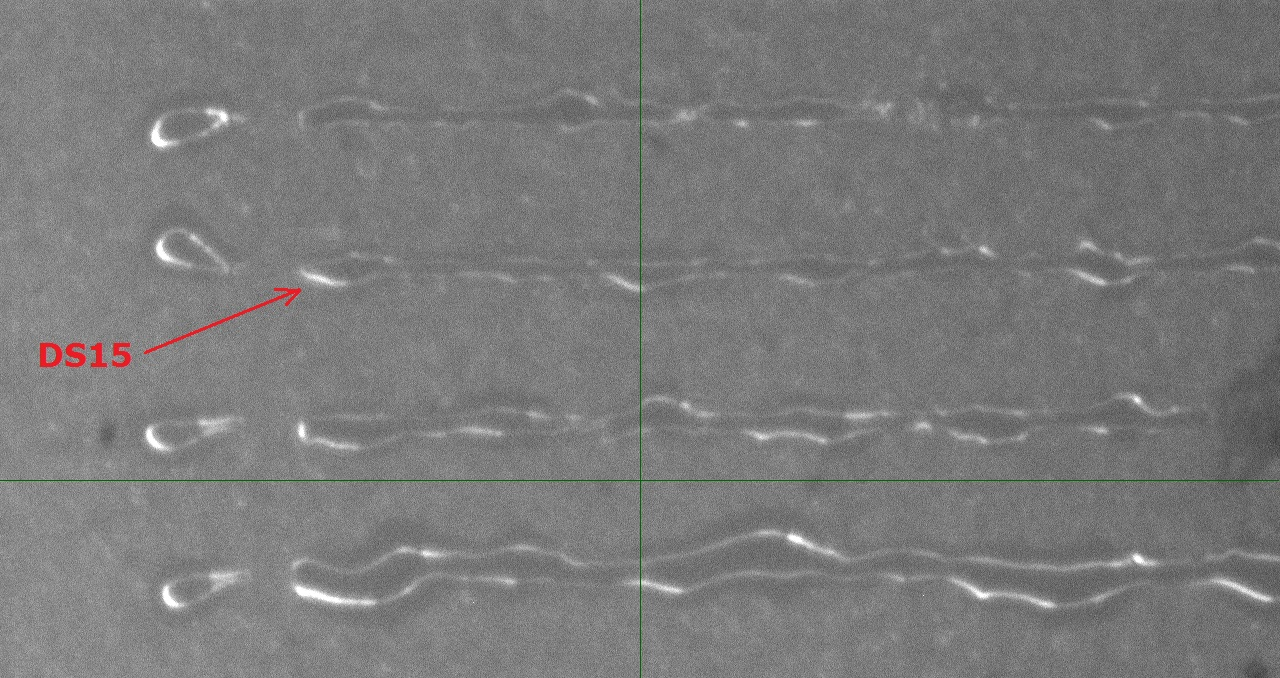
\includegraphics[width=0.5\textwidth]{Figuras/Figura_LinePattern_SU8}
  \caption{Imagen ampliada de impresión $``$\textit{Line Pattern}$"$.}
  \label{fig:Figura_LinePattern_SU8}
\end{figure}

Para este DS es necesario que los archivos a imprimir tengan una resolución de 1693,33 dpi como se vio anteriormente en el Capítulo 3, \hyperref[sec:calib_impresora]{apartado 3.2}.

Una vez configurados los archivos importados mediante el softare \textit{DMP}, se procedió a imprimir el primer anillo de radios 1050 $\mu$m interior y 1350 $\mu$m exterior (Figura ~\ref{fig:Figura_Anillo105a135_SU8}).

\begin{figure}[H]
  \centering
    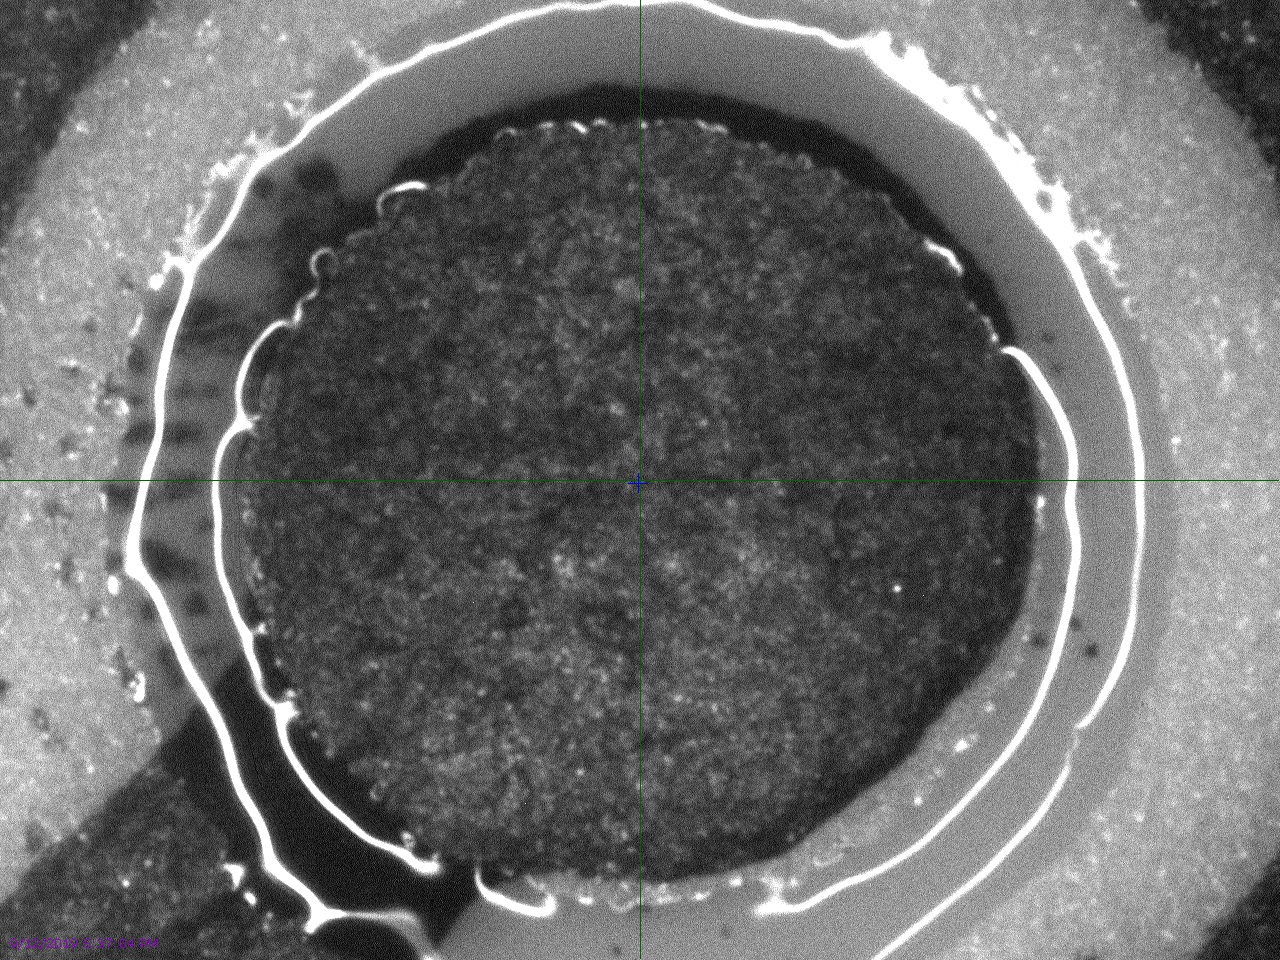
\includegraphics[width=0.5\textwidth]{Figuras/Figura_Anillo105a135_SU8}
  \caption{Impresión anillo de radios 1050 $\mu$m interior y 1350 $\mu$m exterior.}
  \label{fig:Figura_Anillo105a135_SU8}
\end{figure}

Posteriormente, se imprimió un anillo de radios 1100 $\mu$m y 1300 $\mu$m de radios interior y exterior respectivamente (Figura ~\ref{fig:Figura_Anillo110a130_SU8}).

\begin{figure}[H]
  \centering
    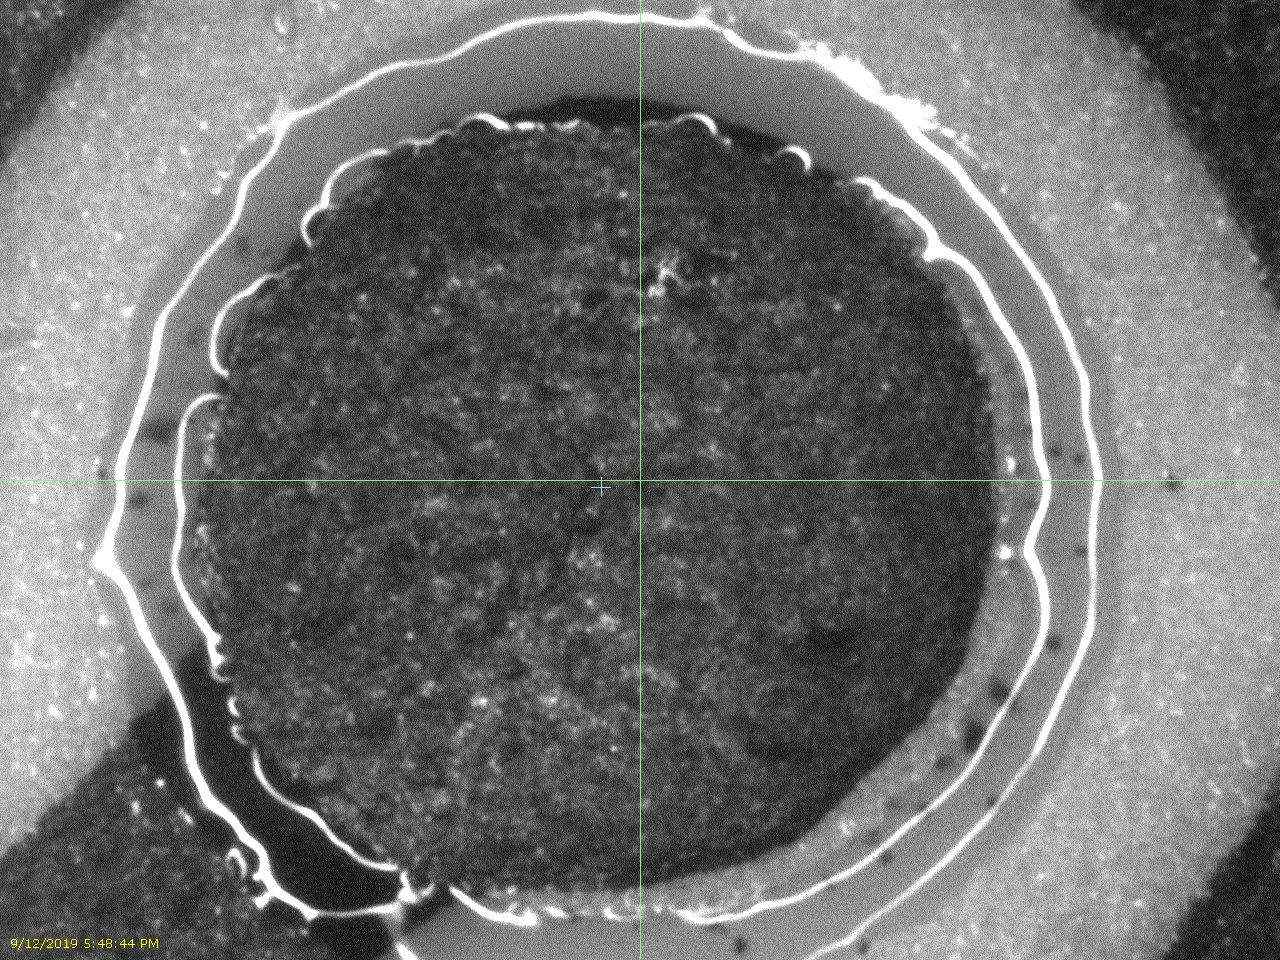
\includegraphics[width=0.5\textwidth]{Figuras/Figura_Anillo110a130_SU8}
  \caption{Impresión anillo de radios 1100 $\mu$m interior y 1300 $\mu$m exterior.}
  \label{fig:Figura_Anillo110a130_SU8}
\end{figure}

Por último, se imprimió el anillo de radios 1150 $\mu$m y 1250 $\mu$m interior y exterior (Figura ~\ref{fig:Figura_Anillo115a125_SU8}).

\begin{figure}[H]
  \centering
    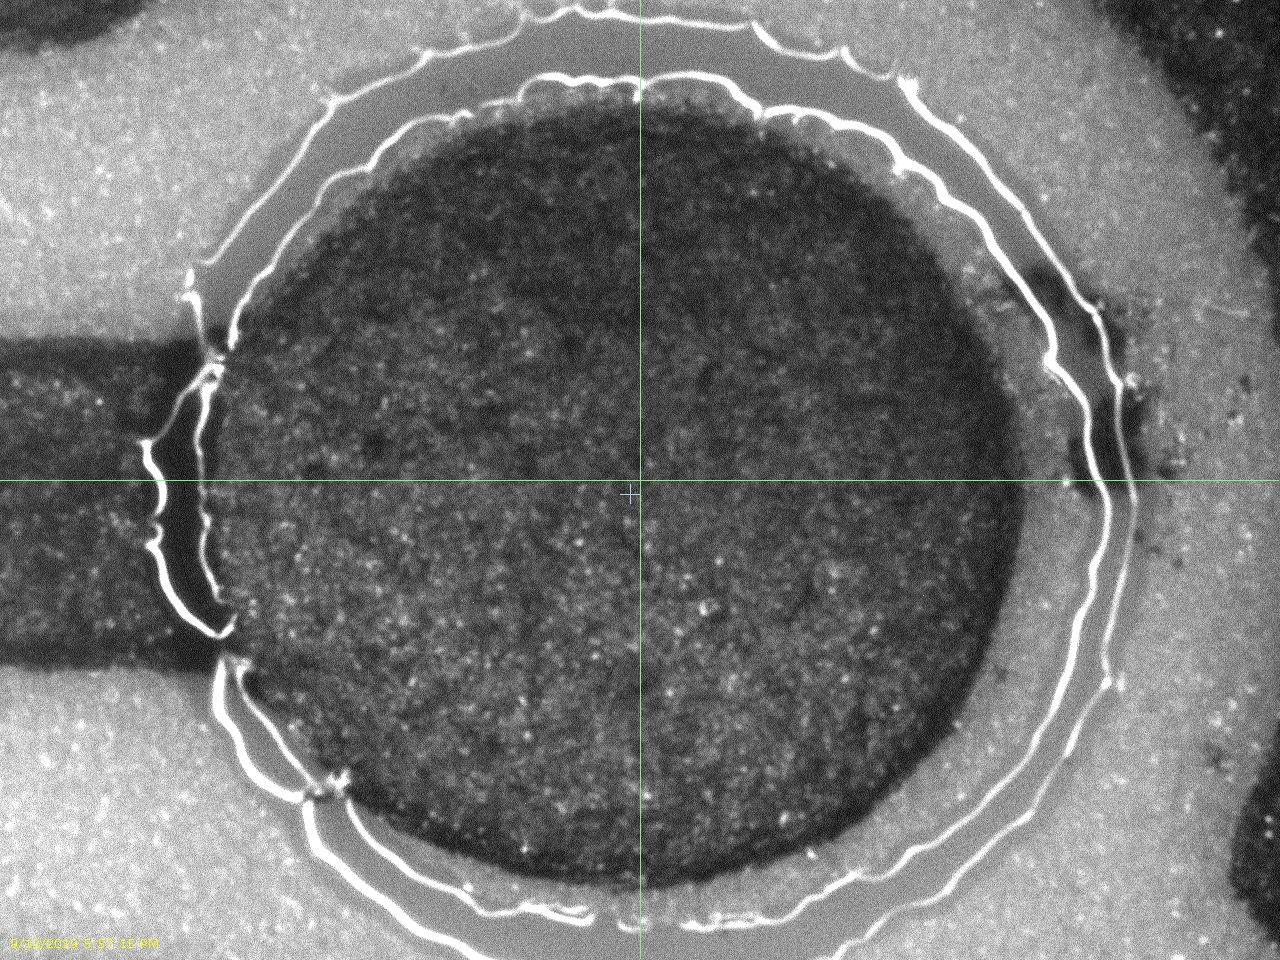
\includegraphics[width=0.5\textwidth]{Figuras/Figura_Anillo115a125_SU8}
  \caption{Impresión anillo de radios 1150 $\mu$m interior y 1250 $\mu$m exterior.}
  \label{fig:Figura_Anillo115a125_SU8}
\end{figure}

\subsection{Caracterizaciones}
Todas las nuevas configuraciones de celdas electroquímicas con microcubetas, obtenidas por impresión \textit{inkjet} con tintas \textit{ad hoc}, serán caracterizadas en un trabajo futuro.